%Textformatierung
\documentclass[a4paper,12pt]{book}
\usepackage[top=1.5cm, left=2cm, right=2cm, bottom=1.5cm, includeheadfoot]{geometry}
\usepackage[utf8]{inputenc}
\usepackage{setspace}
\usepackage[headsepline,nouppercase]{scrlayer-scrpage}

%Hyperlinks
\usepackage{hyperref}
\usepackage[numbers,sort&compress]{natbib}

%Appendix
\usepackage[toc,page]{appendix}

%Mathematik
\usepackage{amsmath}
\allowdisplaybreaks
\usepackage{amsfonts}
\usepackage{amssymb}
\usepackage{verbatim}
\usepackage{slashed}
\usepackage{braket}
\usepackage{dsfont}
\usepackage{subfigure}
\usepackage{array,booktabs}


%Bildverwaltung
\usepackage{axodraw4j}
\usepackage{graphicx}
\usepackage{grffile}
\usepackage[export]{adjustbox}
%\usepackage{subcaption}
%Größe der 3-Nebeneinander-Graphen
\newcommand{\gSize}{6.3cm}
\usepackage[strict]{changepage}
\usepackage{multirow}
%Horizontale Linie
\newcommand{\HRule}{\rule{\linewidth}{0.5mm}}
\usepackage{auto-pst-pdf} 
%Quellcode
\usepackage{listings}
\usepackage{color}
\definecolor{light-gray}{gray}{0.5}
\definecolor{greenly}{rgb}{0,0.2,0}
\usepackage[width=0.8\textwidth,labelfont=bf,font=small]{caption}
\usepackage{xcolor,colortbl}

\lstdefinestyle{customc}{
  belowcaptionskip=1\baselineskip,
  breaklines=true,
  frame=tb,
  numbers=left,
  numberstyle=\color{light-gray},
  xleftmargin=\parindent,
  language=C,
  showstringspaces=false,
  %code-Farben
  basicstyle=\footnotesize\ttfamily,
  commentstyle= \color{light-gray},
  keywordstyle= \color{blue},
  stringstyle= \color{greenly}
}

\lstset{style = customc}

\usepackage{sectsty}
\chapternumberfont{\Large} 
\chaptertitlefont{\Large}
\usepackage{titlesec}

\titleformat{\section}
  {\normalfont\large\bfseries}{\thesection}{1em}{}
  
\titleformat{\subsection}
  {\normalfont\large\bfseries}{\thesubsection}{1em}{}


\makeatletter
\def\@makechapterhead#1{%
  \vspace*{50\p@}%
  {\parindent \z@ \raggedright \normalfont
    \ifnum \c@secnumdepth >\m@ne
      \if@mainmatter
        %\huge\bfseries \@chapapp\space \thechapter
        \Large\bfseries \thechapter \space \space%
        %\par\nobreak
        %\vskip 20\p@
      \fi
    \fi
    \interlinepenalty\@M
    \Large \bfseries #1\par\nobreak
    \vskip 20\p@
  }}
\makeatother

\setkomafont{pagehead}{%
\normalfont}

\renewcommand*\chaptermarkformat{\thechapter. } 

\lstset{breaklines=true,
  breakatwhitespace=true,
  stepnumber=1,
  basicstyle=\ttfamily\footnotesize,
  commentstyle=\ttfamily\color{gray},
  prebreak={\textbackslash},
  breakindent=10pt,
  breakautoindent=false,
  showspaces=false,
  showstringspaces=false,
  frame=shadowbox,
  rulesepcolor=\color{gray},
  rulesep=0.1em,
  abovecaptionskip=0em,
  aboveskip=1.5em,
  belowcaptionskip=0.5em,
  belowskip=1em,
}
\makeatletter
\lstnewenvironment{numlstlisting}[1][]{%
  \lstset{%
    #1,
    numbers=left,
    firstnumber=auto,
    numberstyle=\tiny\sffamily}%
  \csname\@lst @SetFirstNumber\endcsname
}{%
  \csname \@lst @SaveFirstNumber\endcsname
}
%%%%%%%%%%%%%%%%%%%%%%%%%%%%%%%%%%%%%%%%%%%%%
\begin{document}
\pagenumbering{roman}
\begin{titlepage}
	\centering
	{\bfseries Masterarbeit \par}
	\vspace{0.1cm}
	{zur Erlangung des Hochschulgrades \par}
	\vspace{0.1cm}
	{Master of Science \par}
	\vspace{0.1cm}
	{im Studiengang Physik \par}
	\vspace{3cm}
	{\bfseries\Large Complete Calculation of\\ the Dominant Three-Loop Contributions to the\\ Higgs Mass in the 		Standard Model \par}
	\vspace{3cm}
	{vorgelegt am\par}
	\vspace{0.1cm}
	{Institut für Theoretische Teilchenphysik und Kosmologie\par}
	\vspace{0.1cm}
	{der Fakultät für Mathematik, Informatik und Naturwissenschaften \par}
	\vspace{0.1cm}
	{der RWTH Aachen \par}
	\vspace{3cm}
	{1. Gutachter: Prof. Dr. Michael \textsc{Krämer} \par}
	\vspace{0.1cm}
	{2. Gutachter: Prof. Dr. Robert \textsc{Harlander} \par}
	\vspace{3cm}
	{\bfseries Harun Acaro\u{g}lu \par}
	\vspace{0.1cm}
	{geboren am 13.09.1992 in Duisburg \par}
	\vspace{0.1cm}

	\vfill

% Bottom of the page
	{27. März 2019}
\end{titlepage}
%Seitennummer nicht Anzeigen
\thispagestyle{empty}


\clearpage
%Weißer Text, damit Inhaltsverzeichnis nicht auf Titelblatt gedruckt wird
\textcolor{white}{nichts}

\clearpage

\begin{center}
\textbf{Abstract}\\
\end{center} 
We increase the precision of the EFT Higgs mass prediction of \texttt{HSSUSY} from the \texttt{FlexibleSUSY} package by including loop corrections of order $\mathcal{O}(\alpha_s\alpha_t+\alpha_t^2)$ and order $\mathcal{O}(\alpha_s^4)$ to the top quark mass. The two-loop terms are extracted from a more general pole-to-$\overline{\text{MS}}$ mass relation for the top quark which includes electroweak corrections. We find, that the correction of order $\mathcal{O}(\alpha_s\alpha_t)$ decreases the predicted Higgs mass by $\sim 50$ MeV and that the order $\mathcal{O}(\alpha_t^2)$ term increases it by $\sim 100$ MeV. The four-loop pure QCD correction decreases the predicted Higgs mass by $\sim 100$ GeV and we find that there is a fortuitous cancellation between this term and the order $\mathcal{O}(\alpha_t^2)$ contribution. Further, we give an updated uncertainty estimation for the Higgs mass prediction of \texttt{HSSUSY}. %We find, that the experimentally measured Higgs mass can be predicted within a SUSY scale range of $[2.7,4.4]$ TeV.
A comparison to fixed-order calculations in the full MSSM shows, that the EFT approach yields a more precise Higgs mass prediction for scales above $1.1$ TeV. %A Higgs mass of $M_h=125.09$ GeV is predicted for a SUSY scale of $3.5$ TeV with an uncertainty of $\Delta M_h = 0.76$ GeV. 
\thispagestyle{empty}
\clearpage
\textcolor{white}{nichts}
\thispagestyle{empty}
\clearpage

\pagestyle{scrheadings}
\clearscrheadfoot
\ohead{\headmark}
\automark[section]{chapter}
\ifoot{}
\cfoot{}
\ofoot{\pagemark}
\tableofcontents
\clearpage
\thispagestyle{empty}
\clearpage
\pagenumbering{arabic}
\chapter{Introduction}
The 20\textsuperscript{th} century is of fundamental importance in the history of physics. Beside many worldview changing insights that were gained during that period, physics did also evolve as a science and in an epistemological sense: the discipline \textit{theoretical physics} developed and started to become more and more influential. Many brilliant minds of that period, which today are remembered and honored as such, as well as their insights can be assigned to theoretical physics. Be it \textsc{Albert Einstein} with his famous theory of relativity, \textsc{Werner Heisenberg}, \textsc{Max Born} and \textsc{Erwin Schrödinger} with their contributions to quantum mechanics, \textsc{Paul Dirac} with his relativistic quantum theory of the electron, \textsc{Enrico Fermi} and \textsc{Hideki Yukawa} with their contributions to nuclear physics or \textsc{Richard Feynman} and his work on quantum field theory --- they all worked in the field of theoretical physics.\par
The progress and insights that were made in the above mentioned fields are undoubtedly astonishing achievements of modern science. All the more, it is easy to understand the value of a theory that in some sense is the meeting point and culmination of all these insights: the Standard Model (SM) of particle physics, a (special) relativistic quantum field theory capable of describing three out of four fundamental interactions, namely the electromagnetic, strong and weak interactions. Beside --- or more accurately yet because of --- this property, most of its predictions are in a profound accordance with experimental data.\par
Another very appealing aspect of the SM is that it describes all known elementary particles as a gauge theory. As such, the structure of the SM is determined by symmetries. Additionally, it is successful in giving a unified description of the electromagnetic and the weak interaction, known as electroweak unification. Within the scope of this unification it introduces spontaneous symmetry breaking and predicts the existence of the Higgs boson. Its discovery at the Large Hadron Collider (LHC) in 2012 \cite{higgsmeasurement1,higgsmeasurement2} can be counted as the biggest success of the SM so far.\par
Although the SM gives a well-founded description of nature, it also bears weaknesses. While some weaknesses relate to more formal and theoretical aspects of the SM, like e.g. the strong CP problem \cite{strongcp} and the hierarchy problem \cite{hierarchy}, others are discrepancies between the SM's prediction and observations, like measurements of the b meson decay, measurements of neutrino masses and the existence of dark matter\footnote{Provided dark matter is a new type of matter.}. There are different kinds of proposed solutions for these problems. Some solutions consist of local extensions of the SM, like e.g.\ the Seesaw mechanism \cite{seesaw} as a way to introduce neutrino masses or the Peccei-Quinn mechanism \cite{peccei} as a solution for the strong CP problem (and also dark matter). Others are much more profound and propose that the SM is the low-scale effective theory of a more general, superordinate theory. One of the most elaborated theories in this category is Supersymmetry (SUSY).\par
The word supersymmetry refers to an extension of the symmetry of space-time yielding a fundamental relation between fermions and bosons. One very common SUSY model is the Minimal Supersymmetric Standard Model (MSSM). While the Higgs boson mass or the quartic Higgs self-coupling $\lambda$ respectively, is a free parameter in the SM, the MSSM can actually "predict" its value by giving a relation between $\lambda$ and other couplings. Hence, the above mentioned measurement of the Higgs boson mass at the LHC together with its prediction enables the restriction of MSSM parameters.\par
Such a prediction can be done in the full theory, in a fixed-order calculation, where contributions to the Higgs boson mass from SM as well as SUSY particles are taken into account at the same scale. An alternative approach is the effective field theory (EFT) calculation. Here, the quartic self-coupling $\lambda$ is calculated through a matching of the SM to the MSSM at the SUSY scale and the Higgs boson mass is calculated in the SM at the top mass scale by using renormalization group running. The EFT calculation neglects contributions of order $\mathcal{O}(v^2/M_S^2)$, where $M_S$ is the typical SUSY scale, but allows for a resummation of large logarithmic corrections. Thus, the EFT calculation leads to a more precise prediction of $M_h$ for SUSY scales above $M_S \gtrsim$ 1--2 TeV \cite{susyhd,allanachvoigt,uncertainty}. \par
The EFT calculation of the Higgs boson mass is a highly elaborated field and many computer programs have been developed for this purpose. Such programs are for example \texttt{SusyHD} \cite{susyhd} and also \texttt{HSSUSY}, a spectrum generator from the \texttt{FlexibleSUSY} package \cite{FS,FS2}. \texttt{FlexibleSUSY} is a spectrum generator generator that provides a well suited framework for phenomenological studies of SUSY and non-SUSY models. In \texttt{FlexibleSUSY}, dominant SM three-loop corrections to the Higgs mass of order $\mathcal{O}(\alpha_s^2 \alpha_t, \alpha_s \alpha_t^2, \alpha_t^3)$, where $\alpha_s = g_s^2/(4\pi)$ and $\alpha_t = y_t^2/(4\pi)$, are included. However, SM loop corrections for the top quark mass of order $\mathcal{O}(\alpha_s \alpha_t, \alpha_t^2)$, which contribute to the Higgs mass at order $\mathcal{O}(\alpha_s \alpha_t^2, \alpha_t^3)$, are not. In this work, these terms will be extracted from a known two-loop relation between the $\overline{\text{MS}}$ and the pole mass for the top quark \cite{martinmain} and included into the Higgs mass calculation to study their size. The inclusion of these terms will complete the Higgs mass prediction at the currently incomplete three-loop order $\mathcal{O}(\alpha_s\alpha_t^2,\alpha_t^3)$ and thus yield a higher precision for the prediction. This enables the calculation of more precise bounds on the SUSY parameter space. Finally, an updated uncertainty estimation for the EFT Higgs mass prediction will be made.\par
This thesis will begin with two short theory chapters. The SM will be covered in ch.\ \ref{chapter::SM} and the MSSM in ch.\ \ref{chapter::MSSM}. Ch.\ \ref{chapter::FS} will introduce \texttt{FlexibleSUSY} with a special emphasis on the EFT calculation \texttt{HSSUSY} in sec.\ \ref{sec::HS}. The extraction of the relevant terms and their analysis will be presented in ch.\ \ref{chapter::extraction}. In ch.\ \ref{chapter::uncertainty}, the extracted terms as well as the four-loop quantum chromodynamics (QCD) contribution to the top quark mass will be included into the EFT calculation of the Higgs mass and studied. Finally, the Higgs mass uncertainty will be estimated based on these new terms. 
\clearpage
\chapter{The Standard Model of Particle Physics}
\label{chapter::SM}
The SM is a (special) relativistic quantum field theory which describes local interactions of gauge fields with themselves, fermion fields and scalar fields as well as interactions of scalar fields with themselves. Thus, it is also a gauge theory. As such it is based on the local gauge group $\text{SU(3)}_{ \text{C}} \otimes \text{SU(2)}_{ \text{L}} \otimes \text{U(1)}_{ \text{Y}}$. This means, that any interaction term in the SM Lagrangian density $\mathcal{L}_\text{SM}$ has to be invariant under the symmetry transformation of this group. Another central aspect of the SM is, that the above mentioned symmetry group is spontaneously broken down to $\text{SU(3)}_{\text{C}} \otimes \text{U(1)}_{\text{Q}}$ at the electroweak scale $v$. This is known as electroweak symmetry breaking (EWSB).\par
This chapter will shortly review the SM's gauge groups and fields to give the full SM Lagrangian density $\mathcal{L_\text{SM}}$ in gauge eigenstates, i.e.\ before EWSB. Since the very starting point of the analysis in ch.\ \ref{chapter::extraction} is a two-loop relation between the $\overline{\text{MS}}$ mass and the pole mass for the top quark, a short review of how such a relation is calculated will be presented at the one-loop level. 
\section{Gauge Symmetries of the SM}
\subsection{Gauge Group $\normalfont \text{SU(3)}_{ \text{C}}$}
The generators of the gauge group $\text{SU(3)}_{ \text{C}}$ satisfy the Lie algebra
\begin{equation}
\label{eq::Lie-algebra}
[T^a,T^b] = i f^{abc} T^c,
\end{equation}
where the $f^{abc}$ are called structure constants. As its structure constants are non-zero, $\text{SU(3)}_{ \text{C}}$ can be classified as a non-Abelian Lie group. The index "C" refers to the color charge $c$ that this group is associated with.\par
In the SM, $\text{SU(3)}_{ \text{C}}$ is the gauge symmetry of QCD. In QCD the group generators $T^a$ are related to the Gell-Mann matrices 
\begin{equation}
T^a = \frac{\lambda^a}{2},
\end{equation}
where $a \in \{1,...,8\}$. The components of the gluon field strength tensor $G_{\mu\nu}^a$ read
\begin{equation}
G_{\mu\nu}^a = \partial_\mu G_\nu^a - \partial_\nu G_\mu^a + g_s f^{abc} G_\mu^b G_\nu^c, 
\end{equation}
where $g_s$ is the strong coupling constant and 
\begin{equation}
G_\mu=G_\mu^a \frac{\lambda^a}{2}
\end{equation} 
is the gluon gauge field. The covariant derivative $D_\mu$ of a quark field $\psi$ in this representation is given by
\begin{equation}
\label{eq::COSU3}
D_\mu \psi = \left(\partial_\mu - i g_s G_\mu^a \frac{\lambda^a}{2}\right)\psi.
\end{equation} 
Under an infinitesimal $\text{SU(3)}_\text{C}$ gauge transformation
\begin{equation}
U(x) = e^{-\frac{i}{2} \lambda^a \alpha^a(x)}
\end{equation}
the gauge field $G_\mu^a$ and the quark field $\psi$ transform like
\begin{eqnarray}
\psi &\rightarrow& \psi -\frac{i}{2} \lambda^a \alpha^a(x) \psi, \\
G_\mu^a &\rightarrow& G_\mu^a - \frac{1}{g_s}\partial_\mu \alpha^a(x)+f^{abc}\alpha^b(x) G_\mu^c.
\end{eqnarray}
For the covariant derivative this yields
\begin{equation}
D_\mu\psi \rightarrow D_\mu\psi -\frac{i}{2} \lambda^a \alpha^a(x)D_\mu\psi,
\end{equation}
which shows that it transforms like the field itself and therefore preserves gauge invariance. 
\subsection{Gauge Group $\normalfont \text{SU(2)}_{ \text{L}}$}
The group $\text{SU(2)}_{ \text{L}}$ is also a non-Abelian gauge group that satisfies eq.\ \eqref{eq::Lie-algebra}. The charge that is associated with this group is the weak isospin $I$ and the "L" in the index indicates, that the associated gauge boson does only interact with left-handed fermions. In its fundamental representation, the group's generators are given by
\begin{equation}
T^i = \frac{\sigma^i}{2},
\end{equation}
where the $\sigma^i$ are the three Pauli matrices. The structure constants of this group are given by $\epsilon^{abc}$, the completely anti-symmetric tensor in three dimensions. Thus, the components of the field strength tensor read
\begin{equation}
W_{\mu\nu}^i = \partial_\mu W_\nu^i - \partial_\nu W_\mu^i + g \epsilon^{ijk} W_\mu^j W_\nu^k,
\end{equation} 
where $g$ denotes the gauge coupling parameter. The covariant derivative of any left-handed fermion field $\psi_L$ is given by
\begin{equation}
\label{eq::COSU2L}
D_\mu \psi_L = \left(\partial_\mu - i gW_\mu^i \frac{\sigma^i}{2} \right)\psi_L.
\end{equation}
\subsection{Gauge Group $\normalfont \text{U(1)}_{ \text{Y}}$}
This gauge group is an Abelian Lie group and is associated with the weak hypercharge $Y$. The field strength tensor of its gauge field is given by
\begin{equation}
B_{\mu\nu}= \partial_\mu B_\nu - \partial_\nu B_\mu,
\end{equation}
and the covariant derivative of any fermion field $\psi$ is 
\begin{equation}
\label{eq::COU1}
D_\mu  \psi = \left(\partial_\mu + i g^\prime B_\mu \frac{Y}{2}\right)\psi.
\end{equation}
Here, $Y$ is the hypercharge operator of the field $\psi$. Note the different sign convention in eq.\ \eqref{eq::COU1} when compared to eqs.\ \eqref{eq::COSU3} and \eqref{eq::COSU2L}. This convention has to be used to get the usual definition for the electromagnetic charge operator $Q$ known as the \textit{Klein-Nijishima relation}\footnote{This relation can be found by expressing the total covariant derivative from eq.\ \eqref{eq::COtotal} in terms of the mass eigenstates from eq.\ \eqref{eq::masseigenstates}. Then, the prefactor of the photon field $A_\mu$ divided by $i\,e$ gives the charge operator $Q$.}: 
\begin{equation}
\label{eq::klein-nijishima}
Q=\frac{\sigma_3}{2}+\frac{Y}{2}.
\end{equation}
\section{The SM Lagrange Density}
\subsection{Fields of the SM}
The kinetic terms of the SM's gauge fields read
\begin{equation}
\label{eq::Lgauge}
\mathcal{L}_{\text{Gauge}}=-\frac{1}{4}G_{\mu\nu}^a G^{a,\mu\nu} -\frac{1}{4}W_{\mu\nu}^i W^{i,\mu\nu} -\frac{1}{4}B_{\mu\nu} B^{\mu\nu},
\end{equation}
where the field strength tensors are defined as in the preceding sections.\par
Since $\text{SU(2)}_\text{L}$ interactions are only allowed for left-handed spinors, it is convenient to write the kinetic terms for fermions as
\begin{equation}
\label{eq::Lfermion}
\mathcal{L}_{\text{Fermion}} = i \bar{L}^j_L\gamma^\mu D_\mu L^j_L+i \bar{Q}^j_L\gamma^\mu D_\mu Q^j_L+i \bar{e}^j_R\gamma^\mu D_\mu e^j_R+i \bar{u}^j_R\gamma^\mu D_\mu u^j_R + i \bar{d}^j_R\gamma^\mu D_\mu d^j_R.
\end{equation}
Note that in this notation $L$ and $Q$ are the $\text{SU(2)}_\text{L}$ doublets and the superscript $j$ indicates summation over generations. The indices $R/L$ denote the right-handed and left-handed part of Dirac spinors. For a generic Dirac spinor $\Psi$ they are defined as
\begin{equation}
\Psi_{L/R} = \frac{1}{2}(\mathds{1}\mp \gamma^5)\Psi,
\end{equation}
with $\gamma^5$ being the chirality operator. Also, the Dirac adjoint spinor $\bar{\Psi}$ is defined as
\begin{equation}
\bar{\Psi} = \Psi^\dagger \gamma^0.
\end{equation}
\begin{table}[h]
\begin{center}
\renewcommand{\arraystretch}{1.5}
\begin{tabular}{| c | c | c |}
\hline
\multicolumn{3}{| c |}{\textbf{Field content of the SM}}\\
\hline
\hline 
Name& Symbol& $\text{SU(3)}_{ \text{C}}, \text{SU(2)}_{ \text{L}}, \text{U(1)}_{ \text{Y}}$\\
\hline
\multicolumn{3}{| c |}{Fermions (spin 1/2)}\\
\hline
left-handed quarks& $Q^j_L$& $(\textbf{3},\textbf{2},\frac{1}{6})$\\
right-handed  up-type antiquarks& $\bar{u}^j_R$& $(\bar{\textbf{3}},\textbf{1},-\frac{2}{3})$\\
right-handed down-type antiquarks& $\bar{d}^j_R$& $(\bar{\textbf{3}},\textbf{1},\frac{1}{3})$\\
left-handed leptons& $L^j_L$& $(\textbf{1},\textbf{2},-\frac{1}{2})$\\
right-handed antileptons& $\bar{e}^j_R$& $(\textbf{1},\textbf{1},-1)$\\
\hline
\multicolumn{3}{| c |}{Vector bosons (spin 1)}\\
\hline
gluon & $g$ & $(\textbf{8},\textbf{1},0)$\\
W boson & $W^0,W^\pm$& $(\textbf{1},\textbf{3},0)$\\
B boson & $B^0$& $(\textbf{1},\textbf{1},0)$\\
\hline
\multicolumn{3}{| c |}{Scalar boson (spin 0)}\\
\hline
Higgs boson & $\Phi$ & $(\textbf{1},\textbf{2},1)$\\
\hline
\end{tabular}
\caption{Field content of the SM. The last column describes the representations of the SM gauge group: e.g. the symbol $\textbf{1}$ indicates, that a field does not participate in the interaction that is associated with the respective gauge group. In the case of $\text{SU(3)}_\text{C}$ the symbols $\textbf{3}$ and $\bar{\textbf{3}}$ denote the fundamental and anti-fundamental representations $T^a=\lambda^a/2$ and $T^a_\text{anti}=-(\lambda^a)^T/2$ of $\text{SU(3)}_\text{C}$. The notation $\textbf{2}$ is used, when the generators of the group are in their fundamental representation and the last number gives the respective field's value of $Y/2$. The index $j\in \{1,2,3\}$ indicates the existence of three generations.}
\label{tab::SMcontent}
\end{center}
\end{table}
The total covariant derivative for a left-handed fermion $\psi_L$ reads
\begin{equation}
\label{eq::COtotal}
D_\mu  \psi_L = \left(\partial_\mu - i g_s G_\mu^a \frac{\lambda^a}{2} - i g W_\mu^i \frac{\sigma^i}{2} + i {g^\prime} B_\mu \frac{Y}{2}\right)\psi_L,
\end{equation}
while for a right handed fermion it is
\begin{equation}
D_\mu  \psi_R = \left(\partial_\mu - i g_s G_\mu^a \frac{\lambda^a}{2} + i {g^\prime} B_\mu \frac{Y}{2}\right)\psi_R. 
\end{equation}
Tab.\ \ref{tab::SMcontent} gives an overview of the SM's field content.
\subsection{The Higgs Sector and EWSB}
The Lagrangian density of the Higgs sector $\mathcal{L}_\text{Higgs}$ includes a scalar $\text{SU(2)}_\text{L}$ doublet 
  \begin{align}
    \Phi &= \begin{pmatrix}
           \phi^+ \\
           \phi^0 
         \end{pmatrix},
  \end{align}
and a potential 
\begin{equation}
V_\text{Higgs}(\Phi) = -\mu^2 \Phi^\dagger \Phi + \frac{\lambda}{2} \left(\Phi^\dagger \Phi\right)^2.
\end{equation} 
The full expression is given by 
\begin{equation}
\label{eq::Lhiggs}
\mathcal{L}_\text{Higgs} = (D^\mu\Phi)^\dagger (D_\mu\Phi) + \mu^2 \Phi^\dagger \Phi - \frac{\lambda}{2} \left(\Phi^\dagger \Phi\right)^2.
\end{equation}
For $\mu^2>0$ the potential has a non-zero minimum. Then, the scalar field $\Phi$ can be written in terms of its vacuum expectation value (vev) $v = \sqrt{\frac{2\mu^2}{\lambda}}$: 
\begin{align}
\label{eq::scalarSU2doublet}
    \Phi &= \frac{1}{\sqrt{2}}e^{i\frac{\pi^a \sigma^a}{v}} \begin{pmatrix}
           0 \\
           v+h(x) 
         \end{pmatrix}.
\end{align}
The ground state of this doublet is not gauge invariant and breaks the $\text{SU(2)}_{ \text{L}} \otimes \text{U(1)}_{ \text{Y}}$ symmetry. This is known as \textit{spontaneous electroweak symmetry breaking}. Note that even after EWSB the ground state of $\Phi$ is still invariant under the transformation 
\begin{equation}
\Phi_0 \rightarrow e^{i\alpha(x)Q}\Phi_0 = \Phi_0,
\end{equation}
with the ground state 
\begin{align}
    \Phi_0 &= \frac{1}{\sqrt{2}}\begin{pmatrix}
           0 \\
           v 
         \end{pmatrix},
\end{align}
and the charge operator $Q$ defined as in eq.\ \eqref{eq::klein-nijishima}. This remaining symmetry is the $\text{U(1)}_\text{Q}$ gauge symmetry of quantum electrodynamics (QED).\par
The $\pi^a$ in eq. \eqref{eq::scalarSU2doublet} are the Goldstone bosons and depend on the gauge choice. Hence, they are unphysical. In this work, the Goldstone bosons will be denoted by $G^0$ and $G^\pm$. After EWSB one is left with five remaining physical bosons. Four of them can be read off of the ground state's kinetic term
\begin{equation}
(D^\mu\Phi_0)^\dagger (D_\mu\Phi_0) = \frac{v^2}{8}\left[g^2((W_\mu^1)^2 + (W_\mu^2)^2)+ ({g^\prime} B_\mu + g W_\mu^3)^2\right].
\end{equation}
After diagonalizing this matrix one finds the mass eigenstates
\begin{equation}
\label{eq::masseigenstates}
    \begin{pmatrix}
    	A_\mu\\
    	Z_\mu
	\end{pmatrix} = 
	\begin{pmatrix}
    -W_\mu^3 \sin\theta_W + B_\mu \cos\theta_W      \\
    W_\mu^3 \cos\theta_W + B_\mu \sin\theta_W       
	\end{pmatrix}, \quad W_\mu^\pm = \frac{1}{\sqrt{2}}(W_\mu^1 \mp i W_\mu^2),
\end{equation}
with $A_\mu$ being massless and $Z_\mu, W_\mu^\pm$ being massive. The angle $\theta_W$ is called \textit{Weinberg angle} and satisfies
\begin{equation}
\tan\theta_W = \frac{{g^\prime}}{g}. 
\end{equation}
The mass of the three bosons $Z_\mu$ and $W_\mu^\pm$ can be read off from $\mathcal{L}_\text{gauge}$ after rewriting it in terms of the mass eigenstates from eq \eqref{eq::masseigenstates}. One finds
\begin{equation}
m_W = \frac{g v}{2}, \quad \text{and} \quad m_Z = \frac{\sqrt{g^2 + {g^\prime}^2} v}{2}.
\end{equation}
The last physical boson that remains after EWSB is the Higgs boson $h$. By expanding the full kinetic term one finds
\begin{equation}
(D^\mu\Phi)^\dagger (D_\mu\Phi) = - \frac{1}{2} h(\Box + 2 \mu^2)h + ...,
\end{equation} 
which yields 
\begin{equation}
m_h = \sqrt{2}\mu = v \sqrt{\lambda}.
\end{equation}
The same formalism is also used for fermion mass terms in the Lagrangian density. The Lagrangian density for fermion mass terms reads
\begin{equation}
\label{eq::Lyukawa}
\mathcal{L}_\text{Yukawa} = -y_\ell^{ij}\bar{L}_L^i \Phi e_R^j -y_u^{ij}\bar{Q}_L^i \Phi^c u_R^j -y_d^{ij}\bar{Q}_L^i \Phi d_R^j,
\end{equation}   
where the $3 \times 3$ matrices $y_f^{ij}$ are called Yukawa matrices. The charge conjugated field $\Phi^c$ is defined as 
\begin{equation}
\Phi^c = i\sigma^2 \Phi^*.
\end{equation}
Applying the formalism of EWSB yields the mass matrices 
\begin{equation}
m_\ell^{ij}=\frac{v}{\sqrt{2}}y_\ell^{ij}, \quad m_u^{ij}=\frac{v}{\sqrt{2}}y_u^{ij}, \quad m_d^{ij}=\frac{v}{\sqrt{2}}y_d^{ij}.
\end{equation}
\subsection{Ghosts and Gauge Fixing}
In order to be able to define gauge boson propagators properly, one needs to fix the gauge of each gauge boson. In this thesis, the gauge fixing is chosen to be 
\begin{equation}
\label{eq::Lfix}
\mathcal{L}_\text{GF} = - \frac{1}{2\xi_s}(\partial^\mu G_\mu^a)^2 - \frac{1}{2\xi_\text{w}}(\partial^\mu W_\mu^i)^2 - \frac{1}{2\xi_\text{Y}}(\partial^\mu B_\mu)^2.
\end{equation}
It is convenient to use the so called $R_\xi$ gauges, where $\xi_s=\xi_\text{w}=\xi_\text{Y} =\xi$.\par
For non-Abelian gauge groups it is also necessary to include additional unphysical fields, called ghosts. The ghost Lagrangian density is given by the Fadeev-Popov prescription \cite{ghosts}:
\begin{align}
\nonumber
\mathcal{L}_\text{Ghost} = &-\bar{c}_s^{\,a} \partial^\mu \partial_\mu c_s^a + g_s f^{abc}(\partial^\mu c_s^a) G_\mu^a c_s^a\\
\label{eq::Lghost}
&-\bar{c}_\text{w}^{\,i} \partial^\mu \partial_\mu c_\text{w}^i + g \epsilon^{ijk}(\partial^\mu c_\text{w}^i) W_\mu^i c_\text{w}^i,
\end{align}
where the index $s$ indicates ghosts associated with $\text{SU(3)}_\text{C}$ and the index $\text{w}$ labels the $\text{SU(2)}_\text{L}$ ghosts. In the case of the Abelian group $\text{U(1)}_\text{Y}$ one has $f^{abc} = 0$. Thus, the $\text{U(1)}_\text{Y}$ ghosts completely decouple from all other particles and can therefore be omitted. 
\subsection{The Total SM Lagrange Density and Conventions}
With the definitions from above, the SM Lagrangian density is given by 
\begin{equation}
\mathcal{L}_\text{SM} = \mathcal{L}_\text{Gauge} + \mathcal{L}_\text{Fermion} + \mathcal{L}_\text{Higgs} + \mathcal{L}_\text{Yukawa} +\mathcal{L}_\text{GF} + \mathcal{L}_\text{Ghost},
\end{equation}
where the explicit terms are given in the eqs. \eqref{eq::Lgauge}, \eqref{eq::Lfermion}, \eqref{eq::Lhiggs}, \eqref{eq::Lyukawa}, \eqref{eq::Lfix} and \eqref{eq::Lghost}.
According to this Lagrangian density, the following definitions will additionally be used throughout this work: 
\begin{align}
\label{eq::massdeft}
t &\equiv m_t^2 = \frac{y_t^2 v^2}{2},\\
\label{eq::massdefb}
b &\equiv m_b^2 = \frac{y_b^2 v^2}{2},\\
\label{eq::massdefh}
h &\equiv m_h^2 = \lambda v^2\\
\label{eq::massdefW}
W &\equiv m_W^2 = \frac{g^2 v^2}{4},\\
\label{eq::massdefZ}
Z &\equiv m_Z^2 = \frac{\sqrt{g^2+{g^\prime}^2} v^2}{4},
\end{align}
where $y_t = y^{33}_u$ and $y_b = y^{33}_d$. All of the masses of eqs.\ \eqref{eq::massdeft}-\eqref{eq::massdefZ} are $\overline{\text{MS}}$ running masses. In general, a capital $M$ will be used for pole masses while a lower case $m$ will denote $\overline{\text{MS}}$ running masses.
\section{Pole-to-$\overline{\text{MS}}$ Mass Relation for the Top Quark} 
In ch. \ref{chapter::extraction} the starting point will be a relation between the top quark pole mass and the $\overline{\text{MS}}$ mass at the two-loop level. To give a short review on how such a relation is calculated in general, this chapter will present the one-loop result in pure QCD.\par
In the most general form, the relation between the pole and the $\overline{\text{MS}}$ mass is given by
\begin{equation}
\label{eq::moverMgeneral}
\frac{m_t}{M_t} = \frac{Z_m^\text{OS}}{Z_m^{\overline{\text{MS}}}},
\end{equation}
where the mass renormalization constants $Z_m$ are defined through
\begin{equation}
\label{eq::renormalmass}
m_t^0 = m_t Z_m^{\overline{\text{MS}}}, \quad \text{and} \quad
m_t^0 = M_t Z_m^\text{OS} .
\end{equation}
Eqs.\ \eqref{eq::moverMgeneral} and \eqref{eq::renormalmass} hold to all orders in perturbation theory. The superscript of the renormalization constants refers to the subtraction scheme that is used: the \textit{modified minimal subtraction scheme} ($\overline{\text{MS}}$) in the case of $m_t$ and the \textit{on-shell scheme} (OS) in the case of $M_t$. In this notation, $m_t^0$ is the bare top quark mass parameter.\par
At one-loop order, the renormalization constants are given by 
\begin{equation}
Z_m^{\overline{\text{MS}}}=1+\delta_m^{\overline{\text{MS}}}, \quad \text{and} \quad
Z_m^\text{OS} = 1+\delta_m^\text{OS},
\end{equation}
with $\delta_m^{\overline{\text{MS}}}$ and $\delta_m^\text{OS}$ being of one-loop order $\mathcal{O}(g_s^2)$. Hence, to derive the desired relation, one needs to calculate these two constants.\par
For this, it is necessary to know the one-loop top quark self-energy in pure QCD. The only Feynman diagram that contributes at this order is shown in fig.\ \ref{fig::qcd1Lselfenergy}. Its calculation can be found in app.\ \ref{ap::selfenergy}. In dimensional regularization the result reads
\begin{align}
\label{eq::selfenergyQCD}
\Sigma^{(1)}(\slashed{p}) &= \frac{\alpha_s}{4\pi} C_F \int^1_0 dx\, ((2-\varepsilon)(1-x)\slashed{p}-(4-\varepsilon) m_{t,R}) \left(\frac{2}{\varepsilon}+\ln \frac{4\pi e^{-\gamma_E}\mu^2}{x(m_{t,R}^2-(1-x)p^2)}\right)\\
&= \frac{\alpha_s}{\pi}C_F \left(\frac{\slashed{p}-4m_{t,R}}{2\varepsilon}+\text{finite}\right),
\end{align}
where $\alpha_s = g_s^2/(4\pi)$ and $m_{t,R}$ is the renormalized mass in general. The factor $\mu$ stems from a substitution of the form $g_s \rightarrow g_s \mu^{(4-d)/2}$, with $d=4-\varepsilon$ and is called \textit{renormalization scale}. The colour factor $C_F$ is defined through $C_F \delta_{ij} = (\lambda^a_{ik} \lambda^a_{kj})/4 = (4/3) \delta_{ij}$.
\begin{figure}[h]
\begin{center}
\includegraphics[width=0.4\textwidth]{src/feynman/qcd1Lselfenergy.ps}
\caption{The one-loop QCD self-energy diagram of the top quark.}
\label{fig::qcd1Lselfenergy}
\end{center}
\end{figure}\\
The bare top quark propagator is given by 
\begin{equation}
iS^0(\slashed{p})=\frac{i}{\slashed{p}-m_t^0+\Sigma(\slashed{p})}.
\end{equation}
Here, $\Sigma(\slashed{p})$ is the sum over all one particle irreducible Feynman diagrams. At order $\mathcal{O}(\alpha_s)$ one has 
\begin{equation}
\Sigma(\slashed{p})=\Sigma^{(1)}(\slashed{p}). 
\end{equation}
Renormalizing the top quark propagator up to this order yields
\begin{align}
iS^R(\slashed{p})&=\frac{1}{Z_2}\frac{i}{\slashed{p}-m_t^0+\Sigma^{(1)}(\slashed{p})}\\
&=\left(\frac{1}{1+\delta_2}\right)\frac{i}{\slashed{p}-m_t^0+\Sigma^{(1)}(\slashed{p})}\\
\label{eq::renprop}
&=\frac{i}{\slashed{p}-m_t^0+\delta_2\slashed{p}-\delta_2 m_t^0+\Sigma^{(1)}(\slashed{p})+\mathcal{O}(\alpha_s^2)},
\end{align}
where $Z_2$ is the top quark field renormalization constant defined by
\begin{equation}
\psi^R = \frac{1}{\sqrt{Z_2}}\psi^0 = \frac{1}{\sqrt{1+\delta_2}}\psi^0.
\end{equation}
Again, $\delta_2$ is of one-loop order $\mathcal{O}(\alpha_s)$. Expressing \eqref{eq::renprop} through the renormalized mass by using $m_t^0= m_{t,R} Z_m = m_{t,R} + \delta_m m_{t,R}$ yields
\begin{align}
iS^R(\slashed{p})&=\frac{i}{\slashed{p}-m_{t,R}+\delta_2\slashed{p}-(\delta_2+\delta_m) m_{t,R}+\Sigma^{(1)}(\slashed{p})+\mathcal{O}(\alpha_s^2)}\\
\label{eq::proppole}
&= \frac{i}{\slashed{p}-m_{t,R}+\Sigma_R(\slashed{p})},
\end{align}
with $\Sigma_R(\slashed{p}) = \delta_2\slashed{p}-(\delta_2+\delta_m) m_{t,R}+\Sigma^{(1)}(\slashed{p})+\mathcal{O}(\alpha_s^2)$.\par
In the on-shell renormalization scheme the counterterms $\delta_2$ and $\delta_m$ are chosen in such a way, that the renormalized mass $m_{t,R}$ is the pole of the propagator in eq.\ \eqref{eq::proppole} with residue $i$. Applying the first condition determines the counterterm $\delta_m^\text{OS}$:
\begin{align}
\lim_{\slashed{p}\rightarrow M_t}(\slashed{p}-M_t&+\Sigma_R(\slashed{p})) \stackrel{!}{=} 0\\
\Rightarrow \quad \Sigma_R(&M_t) \stackrel{!}{=}  0. 
\end{align}
Finally, at one-loop order this yields
\begin{align}
\Sigma_R(M_t) &=-\delta_m^\text{OS} M_t + \Sigma^{(1)}(M_t)\stackrel{!}{=}0\\
\Rightarrow \quad \delta_m^\text{OS} &= \frac{1}{M_t}\Sigma^{(1)}(M_t)\\
&=\frac{\alpha_s}{2\pi} C_F \left(-\frac{3}{\varepsilon}-\frac{3}{2}\ln\frac{4\pi e^{-\gamma_E}\mu^2}{M_t^2}-2\right)\\
&= -\kappa g_s^2 C_F  \left(\frac{6}{\varepsilon}+ 3\ln\frac{4\pi e^{-\gamma_E}\mu^2}{M_t^2}+4\right),
\end{align}
where $\kappa = 1/(4\pi)^2$ is the loop factor. In the $\overline{\text{MS}}$ scheme only the $1/\varepsilon$ poles and the factor $\ln (4\pi e^{-\gamma_E})$ in eq.\ \eqref{eq::selfenergyQCD} are subtracted. For $\delta_m^{\overline{\text{MS}}}$ one finds
\begin{align}
\delta_m^{\overline{\text{MS}}} &= -\frac{3 \alpha_s}{4\pi} C_F \left( \frac{2}{\varepsilon}+\ln (4\pi e^{-\gamma_E})\right)\\
&=-\kappa g_s^2 C_F\left( \frac{6}{\varepsilon}+3 \ln (4\pi e^{-\gamma_E})\right).
\end{align}
Now we can use eq.\ \eqref{eq::moverMgeneral} to find the relation between $m_t$ and $M_t$:
\begin{equation}
\frac{m_t}{M_t} = \frac{Z_m^\text{OS}}{Z_m^{\overline{\text{MS}}}} =\frac{1+\delta_m^\text{OS}}{1+\delta_m^{\overline{\text{MS}}}}= \frac{1-\kappa g_s^2 C_F  \left(\frac{6}{\varepsilon}+ 3\ln\frac{4\pi e^{-\gamma_E}\mu^2}{M_t^2}+4\right)}{1-\kappa g_s^2 C_F\left( \frac{6}{\varepsilon}+3 \ln (4\pi e^{-\gamma_E})\right)}.
\end{equation}
Expanding this in $\kappa$ up to one-loop order and setting $C_F = 4/3$ then yields
\begin{equation}
\frac{m_t}{M_t} = 1 - \kappa g_s^2 \left[\frac{16}{3}-4 \overline{\ln}(M_t^2)\right],
\end{equation}
where $\overline{\ln}(M_t^2) = \ln \left(M_t^2/\mu^2\right)$. Also, the relation between $M_t$ and $m_t$ is often given in the form 
\begin{align}
M_t^2 &= m_t^2 \left(\frac{Z_m^{\overline{\text{MS}}}}{Z_m^\text{OS}}\right)^2\\
\label{eq::1LQCDdelta}
&=m_t^2 + \kappa g_s^2 m_t^2 \left[\frac{32}{3}-8 \overline{\ln}(M_t^2)\right]+\mathcal{O}(g_s^4).
\end{align}
Note that it is possible in perturbation theory to express the right hand side of \eqref{eq::1LQCDdelta} only in terms of $m_t$ by inserting $M_t^2$. Expanding up to order $\mathcal{O}(\kappa)$ yields
\begin{equation}
M_t^2 = m_t^2 + \kappa g_s^2 m_t^2 \left[\frac{32}{3}-8 \overline{\ln}(m_t^2)\right] = m_t^2 + \kappa g_s^2 \delta^{(1)}_\text{QCD},
\end{equation}
with $\delta^{(1)}_\text{QCD}=m_t^2 \left[(32/3)-8 \overline{\ln}(m_t^2)\right]$. This type of relation will be referred to as the pole-to-$\overline{\text{MS}}$ mass relation in the following. 
\chapter{The Minimal Supersymmetric Standard Model}
\label{chapter::MSSM}
As mentioned in the introduction, SUSY is a very attractive and highly sophisticated extension of the SM. This chapter will give a brief introduction into the general concepts of SUSY to finally explain in what way the MSSM imposes SUSY on the SM. Most importantly, this chapter will introduce and explain MSSM parameters that are used in this work. 
\section{General Concepts of SUSY}
\subsection{Super-Poincaré Algebra and Superpartners}
The very core idea of SUSY is to extend the space-time symmetry algebra of special relativity by fermionic generators. This symmetry is expressed through the Poincaré group and its generators $J^{\mu\nu}$ and $P^\mu$ which satisfy the Poincaré algebra: 
\begin{align}
[P^\mu,P^\nu]&=0,\\
[P^\mu, J^{\alpha\beta}]&= i(g^{\mu\alpha}P^\beta-g^{\mu\beta}P^\alpha),\\
[J^{\mu\nu},J^{\alpha\beta}]&=i(g^{\nu\alpha}J^{\mu\beta}-g^{\mu\alpha}J^{\nu\beta}+g^{\mu\beta}J^{\nu\alpha}-g^{\nu\beta}J^{\mu\alpha}).
\end{align} 
Now, SUSY extends this algebra by introducing fermionic generators as a Majorana spinor
\begin{equation}
Q=\begin{pmatrix}
Q^\alpha\\
\bar{Q}_{\dot{\alpha}}
\end{pmatrix},
\end{equation}
where $Q^\alpha$ and $\bar{Q}_{\dot{\alpha}}$ are Weyl spinors with $\alpha \in \{1,2\}$. The Weyl spinor $\bar{Q}_{\dot{\alpha}}$ is defined through
\begin{equation}
\bar{Q}^{\dot{\alpha}} = i \sigma^2 Q_\alpha^*.
\end{equation}
The resulting algebra is defined by the relations 
\begin{align}
\{Q_\alpha,\bar{Q}_{\dot{\beta}}\}&=2\sigma^\mu_{\alpha\dot{\beta}}P_\mu,\\
[Q_\alpha,J^{\mu\nu}]&=\frac{1}{2}{\left(\sigma^{\mu\nu}\right)_\alpha}^\beta Q_\beta,\\
[Q_\alpha,P^\mu]&=0,
\end{align} 
with $\sigma^{\mu\nu}= \frac{i}{2}[\gamma^\mu,\gamma^\nu]$ and is called a super-Poincaré algebra.\par
Since the operator $Q$ is fermionic, it transforms bosons into fermions and vice versa. Fields that are related through a transformation 
\begin{equation}
\ket{\text{Fermion}}\stackrel{Q}{\longleftrightarrow}\ket{\text{Boson}}
\end{equation}
are referred to as superpartners and form a supermultiplet. Hence, SUSY theories always introduce a set of new fields and parameters. Different fields within a supermultiplet all share the same quantum numbers, except for their spin. 
\subsection{Soft SUSY Breaking}
As seen above, imposing SUSY on the SM results in the introduction of new particles. Since the Casimir operator $P^\mu P_\mu$ of the super-Poincaré algebra satisfies
\begin{equation}
[P^\mu P_\mu, Q_\alpha] = [P^\mu P_\mu, \bar{Q}_{\dot{\alpha}}]=0,
\end{equation}
all fields within one supermultiplet have the same mass, if SUSY is an exact symmetry. This is clearly contradicting experimental data, since no SUSY particles have been detected yet. Thus, SUSY has to be a broken symmetry.\par
SUSY breaking can be achieved by following the same principles as EWSB. Here, the introduced field is a chiral field, that is being assigned with a vev. In analogy to EWSB, SUSY breaking also gives rise to new mass terms. The interactions that this kind of SUSY breaking introduces do not lead to quadratic divergences and therefore assure the renormalizability of the theory. Hence, this formalism of symmetry breaking is referred to as \textit{soft SUSY breaking} \cite{martinSUSY}. 
\section{The MSSM's Structure}
The MSSM imposes SUSY on the SM in a minimal fashion, i.e. the number of new particles is the smallest possible. In doing so, it uses the following labeling scheme:\par 
The bosonic superpartners of SM fermions (e.g. the top quark $u^3_L$) are labeled with a prefixed letter \textit{s} and their fields are marked by a tilde (e.g. the stop quark $\tilde{u}^3_L$). Note that the indices $L$ and $R$ do not have a meaning for these scalar particles. They only denote the chirality of the associated superpartners.\par
In the case of the fermionic superpartners of SM bosons there is no such labelling scheme. The names of the superpartners of the Higgs boson, gluon, W boson and B boson are higgsino, gluino, wino and bino. Again, superpartner fields are marked by a tilde (e.g. the bino field $\widetilde{B}$).\par
In contrast to the SM, the MSSM contains two $\text{SU(2)}_\text{L}$ Higgs doublets. The structure of its Higgs sector in particular will be presented in the next section. Tab.\ \ref{tab::MSSMchirals} and tab.\ \ref{tab::MSSMvectors} give an overview of the MSSM's field content.
\begin{table}[!h]
\begin{center}
\renewcommand{\arraystretch}{1.5}
\begin{tabular}{| c | c | c | c | c |}
\hline
\multicolumn{5}{| c |}{\textbf{Chiral supermultiplets of the MSSM}}\\
\hline
\hline
\multicolumn{2}{| c |}{Names}& spin 0& spin 1/2&$\text{SU(3)}_{ \text{C}}, \text{SU(2)}_{ \text{L}}, \text{U(1)}_{ \text{Y}}$\\
\hline
squarks, quarks& $Q_L$& $(\tilde{u}_L\quad \tilde{d}_L)$& $(u_L\quad d_L)$& $(\textbf{3},\textbf{2},\frac{1}{6})$\\
(3 generations)& $\bar{u}_R$& $\tilde{u}_R^*$& $u_R^\dagger$& $(\bar{\textbf{3}},\textbf{1},-\frac{2}{3})$\\
& $\bar{d}_R$& $\tilde{d}_R^*$& $d_R^\dagger$& $(\bar{\textbf{3}},\textbf{1},\frac{1}{3})$\\
\hline
sleptons, leptons& $L_L$& $(\tilde{\nu}_L\quad \tilde{e}_L)$& $(\nu_L\quad e_L)$& $(\textbf{1},\textbf{2},-\frac{1}{2})$\\ 
(3 generations)& $\bar{e}_R$& $\tilde{e}_R^*$& $e_R^\dagger$& $(\textbf{1},\textbf{1},-1)$\\ 
\hline 
Higgs, higgsino& $H_u$& $(H_u^+ \quad H_u^0)$& $(\widetilde{H}_u^+ \quad \widetilde{H}_u^0)$& $(\textbf{1},\textbf{2},\frac{1}{2})$\\
& $H_d$& $(H_d^0 \quad H_d^-)$& $(\widetilde{H}_d^0 \quad \widetilde{H}_d^-)$& $(\textbf{1},\textbf{2},-\frac{1}{2})$\\
\hline 
\end{tabular}
\caption{The chiral supermultiplets of the MSSM and their field decomposition. The meaning of the last row is as in Table \ref{tab::SMcontent}.}
\label{tab::MSSMchirals}
\end{center}
\end{table}
\begin{table}[h]
\begin{center}
\renewcommand{\arraystretch}{1.5}
\begin{tabular}{| c | c | c | c |}
\hline
\multicolumn{4}{| c |}{\textbf{Vector supermultiplets of the MSSM}}\\
\hline
\hline
Names& spin 1& spin 1/2&$\text{SU(3)}_{ \text{C}}, \text{SU(2)}_{ \text{L}}, \text{U(1)}_{ \text{Y}}$\\
\hline
gluon, gluino& $g$& $\tilde{g}$& $(\textbf{8},\textbf{1},0)$\\
\hline
W bosons, winos& $W^0, W^\pm$& $\widetilde{W}^0, \widetilde{W}^\pm$& $(\textbf{1},\textbf{3},0)$\\
\hline 
B bosons, binos& $B^0$& $\widetilde{B}^0$& $(\textbf{1},\textbf{1},0)$\\
\hline
\end{tabular}
\caption{The vector supermultiplets of the MSSM.}
\label{tab::MSSMvectors}
\end{center}
\end{table}
\subsection{Higgs Sector}
The MSSM contains two Higgs doublets, since terms like 
\begin{equation}
\Phi \Phi^\dagger \Phi,
\end{equation} 
violate SUSY. Hence, one needs two separate Higgs doublets in order to have both, massive particles and antiparticles.\par
The fact that the MSSM contains two $\text{SU(2)}_\text{L}$ Higgs doublets $H_u= (H_u^+, H_u^0)^T$ and $H_d = (H_d^0, H_d^-)^T$ makes it more complicated to describe EWSB. The Higgs potential of the MSSM reads \cite{martinSUSY}
\begin{align}
V_\text{Higgs} ={}&
(|\mu|^2 + m^2_{H_u}) (|H_u^0|^2 + |H_u^+|^2)
+ (|\mu|^2 + m^2_{H_d}) (|H_d^0|^2 + |H_d^-|^2)
\nonumber \\
&+\, [b\, (H_u^+ H_d^- - H_u^0 H_d^0) + \text{c.c.}]
\nonumber \\
&+ \frac{1}{8} (g^2 + {g^\prime}^2)
(|H_u^0|^2 + |H_u^+|^2 - |H_d^0|^2 - |H_d^-|^2 )^2
+ \frac{1}{2} g^2 |H_u^+ H_d^{0*} + H_u^0 H_d^{-*}|^2 .
\end{align}
The minimum of this potential has to break down the electroweak symmetry to electromagnetism: $\text{SU(2)}_{ \text{L}} \otimes \text{U(1)}_{ \text{Y}} \rightarrow \text{U(1)}_{ \text{Q}}$. Since the gauge symmetry of QED is not broken, the charged components $H_u^+$ and $H_d^-$ of the two Higgs doublets may not acquire a vev. Thus, one can set $\langle H_u^+\rangle=\langle H_d^-\rangle=0$. This leads to the potential 
\begin{align}
\label{eq::MSSMHiggspot}
V_\text{Higgs} ={}&
(|\mu|^2 + m^2_{H_u}) |H_u^0|^2 
+ (|\mu|^2 + m^2_{H_d}) |H_d^0|^2
- (b H_u^0 H_d^0 + \text{c.c.})
\nonumber \\
&+ \frac{1}{8} (g^2 + {g^\prime}^2)
(|H_u^0|^2 - |H_d^0|^2)^2.
\end{align}
Now we can write 
\begin{equation}
v_d = \langle H_d^0\rangle \quad \text{and} \quad v_u = \langle H_u^0\rangle,
\end{equation}
and demand
\begin{equation}
\label{eq::MSSMHiggspotMin}
\frac{\partial V_\text{Higgs}}{\partial H_u^0} \stackrel{!}{=} 0 \quad \text{and} \quad 
\frac{\partial V_\text{Higgs}}{\partial H_d^0} \stackrel{!}{=} 0.
\end{equation}
The MSSM Higgs vevs $v_u$ and $v_d$ are related to the SM vev $v$ through 
\begin{equation}
v_u^2+v_d^2 = v = \frac{2m_Z^2}{g^2+{g^\prime}^2},
\end{equation}
and one additionally defines 
\begin{equation}
\tan\beta = \frac{v_u}{v_d}.
\end{equation} 
Demanding eq. \eqref{eq::MSSMHiggspotMin} then yields the conditions
\begin{align}
m_{H_u}^2 + |\mu |^2 -b \cot\beta - (m_Z^2/2) \cos (2\beta) &= 0,\\
m_{H_d}^2 + |\mu |^2 -b \tan\beta + (m_Z^2/2) \cos (2\beta) &= 0.
\end{align}
Now, one can write the gauge eigenstates in terms of mass eigenstates as \cite{martinSUSY}
\begin{equation}
\begin{pmatrix}
H_u^0\\
H_d^0
\end{pmatrix} =
\begin{pmatrix}
v_u\\
v_d
\end{pmatrix} + 
\frac{1}{\sqrt{2}} \begin{pmatrix}
\cos \alpha& \sin \alpha\\
-\sin \alpha& \cos \alpha
\end{pmatrix} \begin{pmatrix}
h^0\\
H^0
\end{pmatrix}+ 
\frac{i}{\sqrt{2}} \begin{pmatrix}
\sin \beta& \cos \beta\\
-\cos \beta& \sin \beta
\end{pmatrix} \begin{pmatrix}
G^0\\
A^0
\end{pmatrix},
\end{equation}
\begin{equation}
\begin{pmatrix}
H_u^+\\
H_d^{-*}
\end{pmatrix} =
\begin{pmatrix}
\sin \beta& \cos \beta\\
-\cos \beta& \sin \beta
\end{pmatrix} \begin{pmatrix}
G^+\\
H^+
\end{pmatrix}.
\end{equation}
The new fields $G^0$ and $G^\pm$ are the Goldstone bosons, while the two remaining  CP even scalar fields $h^0$ and $H^0$, the remaining CP odd scalar field $A^0$ as well as the charged scalar fields $H^\pm$ are physical. Here, it was defined that $G^- = G^{+*}$ and $H^- = H^{+*}$. By expanding the kinetic part of the Higgs potential one finds
\begin{equation}
V_\text{Higgs} = \frac{1}{2} m_{h^0}^2 (h^{0})^2 + \frac{1}{2} m_{H^0}^2 (H^{0})^2 
+ \frac{1}{2} m_{A^0}^2 (A^{0})^2 +  m_{H^\pm}^2 |H^+|^2 + \cdots,
\end{equation}
yielding the masses
\begin{align}
m_{A^0}^2 &= 2|\mu|^2 + m^2_{H_u} + m^2_{H_d} = \frac{2b}{\sin 2\beta},\\
m^2_{h^0, H^0} &= \frac{1}{2}\left(m^2_{A^0} + m_Z^2 \mp 
\sqrt{(m_{A^0}^2 - m_Z^2)^2 + 4 m_Z^2 m_{A^0}^2 \sin^2 2\beta}\right), 
\label{eq:HiggsmassMSSM}\\
m^2_{H^\pm} &= m^2_{A^0} + m_W^2.
\end{align}
Note that the masses $m_{A^0}, m_{H^0}$ and $m_{H^\pm}$ can become arbitrary large, while $m_{h^0}$ cannot. In this work, $h^0$ will be regarded as the SM-like Higgs boson and thus the superscript \textit{0} will be omitted. Expanding its mass for large $m_{A^0}$ one finds 
\begin{equation}
\label{eq::higgsupperbound}
m^2_h = m_Z^2 \cos^2 2\beta \leq m_Z^2.
\end{equation}  
This is not contradicting Higgs mass measurements, which have shown that its mass is larger than $m_Z$ \cite{higgsmeasurement1,higgsmeasurement2}, since this is just an upper bound on the tree-level mass.\par
Eq.\ \eqref{eq::higgsupperbound} can be used to derive a relation between the SM Higgs self-coupling $\lambda$ and other SM couplings. At tree-level one finds 
\begin{equation}
\lambda = \frac{1}{4}(g^2+{g^\prime}^2)\cos^2 2\beta.
\end{equation} 
This is a key feature of the MSSM, which makes it possible to calculate the Higgs boson mass in the SM using renormalization group running. The details of such a calculation will be presented in ch.\ \ref{chapter::FS}.
\subsection{Sfermion Masses}
The Lagrangian density for sfermion masses is 
\begin{align}
\nonumber
\mathcal{L}_\text{Sfermion} = \sum_{j=1}^3 \biggl[& \left. -\left(\tilde{u}_{L_j}^\dagger \quad \tilde{u}_{R_j}^\dagger\right) M^2_{\tilde{u}_j} \begin{pmatrix}
\tilde{u}_{L_j}\\
\tilde{u}_{R_j}
\end{pmatrix} 
-\left(\tilde{d}_{L_j}^\dagger \quad \tilde{d}_{R_j}^\dagger\right) M^2_{\tilde{d}_j} \begin{pmatrix}
\tilde{d}_{L_j}\\
\tilde{d}_{R_j}
\end{pmatrix}\right.\\
 &-\left(\tilde{e}_{L_j}^\dagger \quad \tilde{e}_{R_j}^\dagger\right) M^2_{\tilde{e}_j} \begin{pmatrix}
\tilde{e}_{L_j}\\
\tilde{e}_{R_j}
\end{pmatrix} - \tilde{\nu}_{L_j}^\dagger m^2_{\tilde{\nu}_j} \tilde{\nu}_{R_j}^\dagger \biggr],
\end{align}
with mass matrices 
\begin{align}
M^2_{\tilde{u}_j} &= \begin{pmatrix}
m_{u_j}^2 + m^2_{\tilde{Q}_j}+m_Z^2 c_{2\beta} \left(I_3-Q s_{\theta_W}^2\right)& m_{u_j} \left(A_{u_j}^*-\mu \cot \beta\right)\\
m_{u_j} \left(A_{u_j}-\mu^* \cot \beta\right)& m_{u_j}^2 + m^2_{\tilde{U}_j}+m_Z^2 c_{2\beta} Q s_{\theta_W}^2
\end{pmatrix},\\
M^2_{\tilde{d}_j} &= \begin{pmatrix}
m_{d_j}^2 + m^2_{\tilde{Q}_j}+m_Z^2 c_{2\beta} \left(I_3-Q s_{\theta_W}^2\right)& m_{d_j} \left(A_{d_j}^*-\mu \tan \beta\right)\\
m_{d_j} \left(A_{d_j}-\mu^* \tan \beta\right)& m_{d_j}^2 + m^2_{\tilde{D}_j}+m_Z^2 c_{2\beta} Q s_{\theta_W}^2
\end{pmatrix},\\
M^2_{\tilde{e}_j} &= \begin{pmatrix}
m_{e_j}^2 + m^2_{\tilde{L}_j}+m_Z^2 c_{2\beta} \left(I_3-Q s_{\theta_W}^2\right)& m_{e_j} \left(A_{e_j}^*-\mu \tan \beta\right)\\
m_{e_j} \left(A_{e_j}-\mu^* \tan \beta\right)& m_{e_j}^2 + m^2_{\tilde{E}_j}+m_Z^2 c_{2\beta} Q s_{\theta_W}^2
\end{pmatrix},
\end{align}
\begin{equation}
\text{and} \quad  m^2_{\tilde{\nu}_j} = m^2_{\tilde{L}_j} + \frac{1}{2} m_Z^2 c_{2\beta},
\end{equation}
with $c_{2\beta} = \cos 2\beta$ and $s_{\theta_W} = \sin\theta_W$. Here, $m^2_{\tilde{Q}_j},  m^2_{\tilde{U}_j}, m^2_{\tilde{D}_j},  m^2_{\tilde{L}_j},  m^2_{\tilde{E}_j}$ as well as $A_{u_j}, A_{d_j}$ and  $A_{e_j}$ are parameters from the soft SUSY breaking sector of the MSSM Lagrangian density. It is convenient to define the parameter
\begin{equation}
X_{u_j} = \left(A_{u_j}^*-\mu \cot \beta\right),
\end{equation}
and especially the important stop mixing parameter 
\begin{equation}
X_t = \left(A_{u_3}^*-\mu \cot \beta\right).
\end{equation}
In this work, we assume a degenerated mass spectrum for SUSY particles 
\begin{equation}
m_{\tilde{Q}_j}^2=m_{\tilde{U}_j}^2=\cdots = \colon M_S^2
\end{equation}
and define
\begin{equation}
\hat{X}_t =\frac{X_t}{(m_{\tilde{Q}_3} m_{\tilde{U}_3})^{(1/2)}}= \frac{X_t}{M_S}.
\end{equation}
The scale $M_S$ is called SUSY scale. An overview for different relevant scales will be given in the second section of the next chapter. 
\chapter{FlexibleSUSY}
\label{chapter::FS}
\section{Overview of the Program}
\texttt{FlexibleSUSY} \cite{FS,FS2} is a sepctrum generator generator, which is suitable for phenomenological studies of SUSY and non-SUSY models specified by its user. It is a \texttt{Mathematica} and \texttt{C++} package, that provides fast and reliable calculations of mass spectra, the anomalous magnetic moment of the muon and further observables. The user can specify the model through an external \texttt{SARAH} \cite{sarah1,sarah2,sarah3,sarah4,sarah5} model file, that contains the super-field content, superpotential, gauge symmetries and mass mixings. The boundary conditions for model parameters are defined through a separate \texttt{FlexibleSUSY.m.in} file. \texttt{FlexibleSUSY} then  uses \texttt{SARAH} for the calculation of mass matrices, vertices, tadpole diagrams, self-energies and renormalization group equations (RGEs) of the specified model. In a second step it converts these algebraic expressions into a \texttt{C++} code.\par
Once the \texttt{C++} code is generated and compiled, the input parameters can be specified via an \texttt{SLHA} file \cite{slha1,slha2}. Model parameters are either defined in the $\overline{\text{MS}}$ or $\overline{\text{DR}}^{\prime}$ scheme. Using this input, the generated spectrum generator then calculates the spectrum of the specified model as well as other observables and writes it into an \texttt{SLHA} output file \cite{FS}. 
\section{High Scale MSSM (HSSUSY)}
\label{sec::HS}
\texttt{HSSUSY} is a spectrum generator from the \texttt{FlexibleSUSY} package. In this model, the SM quartic Higgs self-coupling $\lambda$ is calculated through a matching to the MSSM at a high SUSY scale $M_S$. Thus, this model is very suitable for Higgs mass calculations in a pure EFT approach, where $v^2 \ll M_S^2$ and all SUSY particles are integrated out.\par
There are different scales that are relevant for the Higgs pole mass calculation of \texttt{HSSUSY} (see fig.\ \ref{fig::scales}):
\begin{itemize}
\item{The SUSY scale $M_S$:}\\
This scale is the typical SUSY scale. Non-SM parameters, as well as mass parameters of particles introduced by the MSSM are input at this scale. 
\item{The matching scale $Q_\text{match}$:}\\
The high scale matching between the MSSM and the SM is performed at the matching scale $Q_\text{match}$. At this scale, $\lambda$ is fixed by matching the MSSM to the SM (see below). At default settings, the matching scale is set to $Q_\text{match} = M_S$.
\item{The pole mass scale $Q_\text{pole}$:}\\
This is the scale at which \texttt{HSSUSY} calculates the pole mass spectrum including the Higgs pole mass $M_h$. At default this value is set to the top quark pole mass $Q_\text{pole}=M_t = 173.34$ GeV.
\item{The low scale $Q_\text{low}$:}\\
The SM input parameters are fixed at the low energy scale $Q_\text{low}$ from known low-energy observables like $\alpha_\text{em},\alpha_s,M_Z,M_t,G_F$ etc. The default value for this scale is the Z boson pole mass $Q_\text{low}=M_Z = 91.1876$ GeV.  
\end{itemize}
For the calculation of the Higss pole mass $M_h$, \texttt{HSSUSY} first determines the SM input parameters at the scale $Q_\text{low}$. Then it numerically integrates the SM RGEs up to the matching scale $Q_\text{match}$. At the scale $Q_\text{match}$, \texttt{HSSUSY} calculates the value for $\lambda$ and uses it to re-evaluate the input parameters at $Q_\text{low}$. Next, the value of $\lambda$ is again calculated at the scale $Q_\text{match}$ using the re-evaluated input parameters. This iterative procedure is repeated as many times, as it is required to reach the precision goal, which at default settings is set to $10^{-5}$. Once the parameters have converged up to this precision, \texttt{HSSUSY} uses this set of parameters to calculate the SM pole mass spectrum at the scale $Q_\text{pole}$. The numerical integration of the RGEs introduces infinitely many higher order contributions, which are in general not cancelled by the threshold corrections or loop corrections used to calculate the pole masses.\\
\begin{figure}[h]
\begin{center}
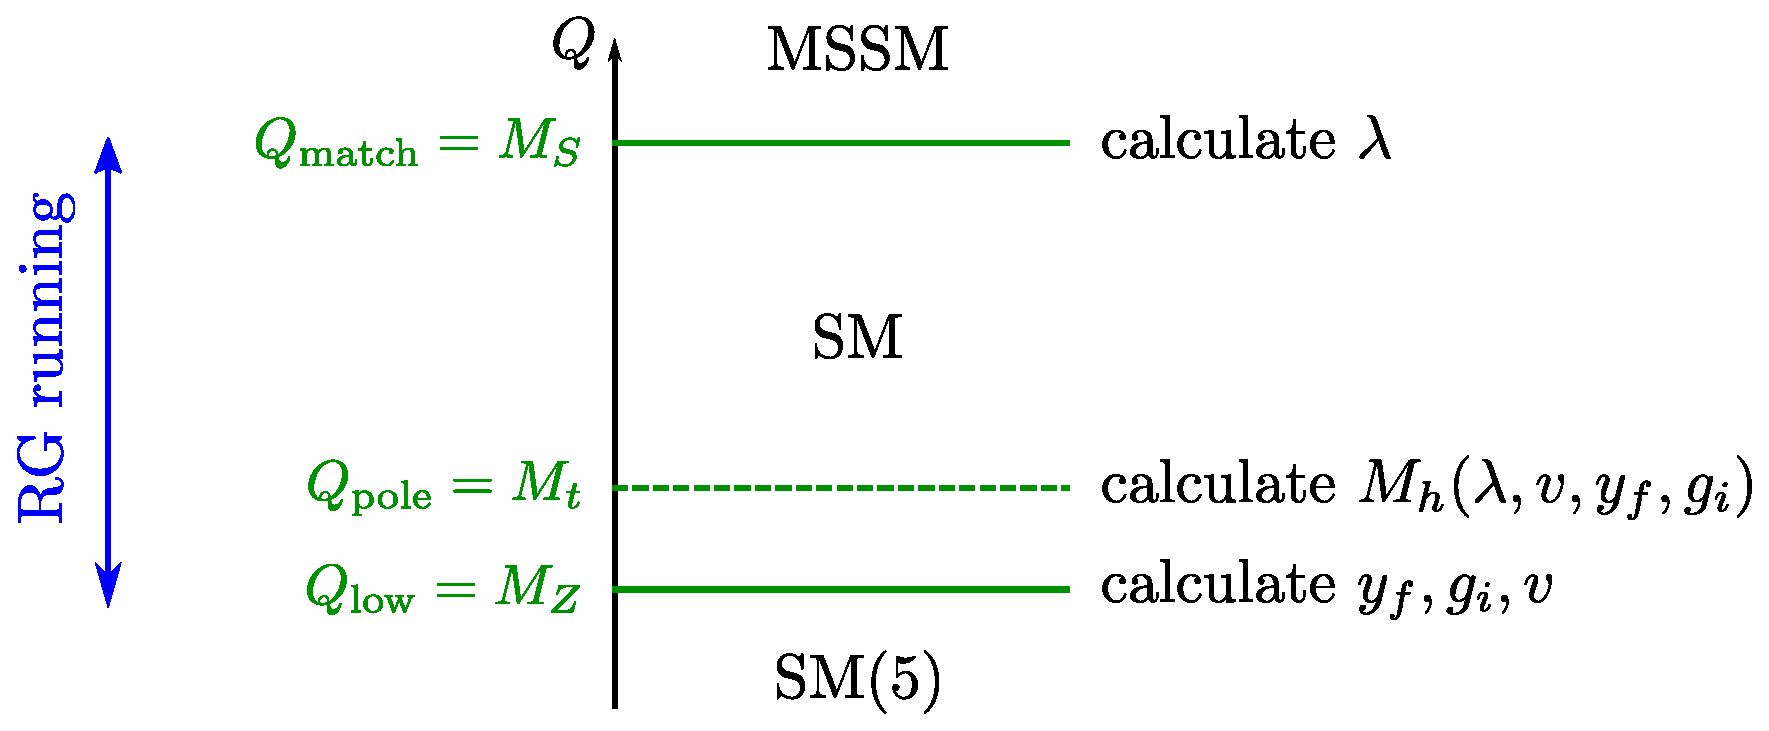
\includegraphics[width=0.85\textwidth]{src/img/scales_HSSUSY.eps}
\caption{This figure gives an overview of the different relevant scales for \texttt{HSSUSY}. The symbol SM(5) denotes the five-flavour SM, where all SM fields except for the top quark are considered.}
\label{fig::scales}
\end{center}
\end{figure}\par
In \texttt{HSSUSY} the matching between the SM and the MSSM is performed up to the three-loop level. For the Higgs self coupling one has 
\begin{equation}
\label{eq::lambdaMS}
\lambda(M_S) = \frac{1}{4}(g^2+{g^\prime}^2)\cos^2 2\beta + \Delta\lambda^{(1)} + \Delta\lambda^{(2)}+ \Delta\lambda^{(3)}. 
\end{equation}
The threshold correction $\Delta\lambda^{(1)}$ is known in the full SM and is obtained from ref.\ \cite{uncertainty}. $\Delta\lambda^{(2)}$ is known at the orders $\mathcal{O}((\alpha_t+\alpha_b)\alpha_s+\alpha_b\alpha_\tau+(\alpha_b+\alpha_t)^2)$ and is obtained from ref.\ \cite{uncertainty,lambda2}. Here, we use $\alpha_b= y_b^2/(4\pi)$ and $\alpha_\tau = (y_\ell^{33})^2/(4\pi)$. The loop correction $\Delta\lambda^{(3)}$ is obtained from ref.\ \cite{lambda3} and is known at the order $\mathcal{O}(\alpha_s^2\alpha_t)$.\par
The SM loop corrections for $M_h$ are known up to the orders $\mathcal{O}(\alpha_t^3 + \alpha_s^2 \alpha_t + \alpha_t^2 \alpha_s)$ at the three-loop level and $\mathcal{O}(\alpha_s^3\alpha_t)$ at the four-loop level \cite{martinHiggs1L,martinHiggs4L,susyhd}. The total expression for $M_h$ reads
\begin{align}
\label{eq::Higgspolemass}
M_h^2 = m_h^2 + (\Delta m_h^2)_{1L}(p^2) + (\Delta m_h^2)_{2L}(p^2) +(\Delta m_h^2)_{3L}+ (\Delta m_h^2)_{4L}.
\end{align}
The full expression of $(\Delta m_h^2)_{1L}(p^2)$ can be found in ref.\ \cite{martinHiggs1L}. It is known in the full SM, i.e.\ it also includes electroweak corrections. Note that the expressions of ref.\ \cite{martinHiggs1L} are restricted to Landau gauge in the electroweak sector (i.e. $\xi=0$) and that the convention $\lambda \rightarrow 2\lambda$ is used. At order $\mathcal{O}(\alpha_t)$ the one-loop correction reads
\begin{align}
\nonumber
(\Delta m_h^2)^{(\alpha_t)}_{1L}(p^2) = \kappa y_t^2 &\left[\frac{3 \left(p^2-4 t\right)}{p} \Bigg(\bigg.p \> \overline{\ln}(t)-2 p\right.\\
\label{eq::dmh1Lat}
&\left.\left.-\sqrt{p^2-4 t} \ln \left(\frac{p
\sqrt{p^2-4 t}-p^2+2 t}{2
   t}\right)\right)\right].
\end{align}
The two-loop contribution splits up as
\begin{equation}
(\Delta m_h^2)_{2L}(p^2) = (\Delta m_h^2)_{2L}^{(\alpha_t^2)} + 
     (\Delta m_h^2)_{2L}^{(\alpha_t\alpha_s)}(p^2),
\end{equation}
with \cite{susyhd,martinHiggs1L}
\begin{align}
\label{eq:2L_Mh_atat}
  (\Delta m_h^2)_{2L}^{(\alpha_t^2)} &= \kappa^2 y_t^4 \left[
    -6 t \left(3 \overline{\ln}^2(t) - 7 \overline\ln(t) + 2 + \frac{\pi^2}{3}\right)
  \right],\\
  \label{eq:2L_Mh_atas}
  (\Delta m_h^2)_{2L}^{(\alpha_t\alpha_s)} (p^2)&=
     \kappa^2 g_s^2 y_t^2 \left[
        \frac{37}{3} p^2 - \frac{122 p^4}{135 t} - 4 (5 p^2 - 8 t) \overline{\ln}(t) -
        12 (p^2 - 8 t) \overline{\ln}^2(t) \right].
\end{align}
The three-loop contribution reads \cite{martinHiggs1L}
\begin{align}
  (\Delta m_h^2)_{3L} ={}&
\kappa^3 \biggl[
     g_s^4 y_t^2 \>t \left(248.122 + 839.197 \>\overline{\ln}(t) + 160 \>\overline{\ln}^2(t) - 736 \>\overline{\ln}^3(t)\right) \nonumber \\
     &+ g_s^2 y_t^4 \>t \left(2764.365 + 1283.716 \>\overline{\ln}(t) - 360 \>\overline{\ln}^2(t) + 240 \>\overline{\ln}^3(t)\right) \nonumber \\
     &+ y_t^6 \>t \bigg(-3199.017 + 36 \>\overline{\ln}(h) - 2653.511 \>\overline{\ln}(t) + 756 \>\overline{\ln}(h) \>\overline{\ln}(t)\bigg. \nonumber \\
     \label{eq::dmh3L}
     &\left.+ \frac{27}{2} \>\overline{\ln}^2(t) + 324 \>\overline{\ln}(h) \>\overline{\ln}^2(t) - 225 \>\overline{\ln}^3(t)\right)\biggr].
\end{align}
In \texttt{FlexibleSUSY}, the corrections of order $\mathcal{O}(\alpha_t)$ and $\mathcal{O}(\alpha_s\alpha_t)$ are implemented with their momentum dependency. \texttt{HSSUSY} performs a momentum iteration, where $p$ is set equal to $M_h$. Thus, this iteration generates additional contributions at higher order.\par
The four-loop correction in eq. \eqref{eq::Higgspolemass} is of order $\mathcal{O}(\alpha_s^3 \alpha_t)$ and can be found in reference \cite{martinHiggs4L}. It reads
\begin{align}
\nonumber
(\Delta m_h^2)_{4L} ={}& \kappa^4\>g_s^6\>y_t^2\>t \biggl[23925.975+6435.327\>\overline{\ln}(t)+20675.746\>\overline{\ln}^2(t)\\
\label{eq::dmh4L}
&+3456\>\overline{\ln}^3(t)+5520\>\overline{\ln}^4(t)\biggr]\,.
\end{align}
The relevant $\beta$-functions for the Higgs mass prediction are the functions $\beta(\lambda),\beta(y_t),\beta(g_s)$ and $\beta(v)$. In \texttt{FlexibleSUSY}, $\beta(g_s)$ is implemented up to the five-loop level, while $\beta(\lambda)$ and $\beta(y_t)$ are implemented up to the four-loop level and $\beta(v)$ is implemented up to the two-loop level \cite{beta1,beta2,beta3,beta4,beta5,martinHiggs4L,beta7,beta8,beta9}.\par 
The running $\overline{\text{MS}}$ top quark mass $m_t$ is implemented up to the orders $\mathcal{O}(\alpha_s+\alpha_t+\alpha_b+\alpha_\text{EW})$ at the one-loop level. Here, $\alpha_\text{EW}$ is defined as $g^2/(4\pi)$. At the two-loop and three-loop levels, the pure QCD contributions of order $\mathcal{O}(\alpha_s^2)$ and $\mathcal{O}(\alpha_s^3)$ are also included. In sec.\ \ref{sec::implementation}, the way $m_t$ is implemented in \texttt{FlexibleSUSY} will be presented in detail. 
\chapter{ Extraction of $\mathcal{O}(\alpha_s \alpha_t+\alpha_t^2)$ Terms for $m_t$}
\label{chapter::extraction}
In ref.\ \cite{martinmain}, a two-loop top quark pole-to-$\overline{\text{MS}}$ mass relation of the form
\begin{equation}
\label{eq::mt2L}
s_\text{pole} = t + \kappa \left(g_s^2 \> \delta^{(1)}_\text{QCD} + \delta^{(1)}_\text{non--QCD}\right)+\kappa^2 \left(g_s^4 \> \delta^{(2)}_\text{QCD}+ g_s^2 \> \delta^{(2)}_\text{mixed,full} + \delta^{(2)}_\text{non--QCD}\right) ,
\end{equation}
was calculated. For the calculation of the one-loop non--QCD contribution, any Yukawa coupling other than $y_t$ and $y_b$ was set to zero, while for the two-loop non--QCD as well as the mixed contribution $y_b$ was also set to zero. The top quark pole mass is defined as 
\begin{equation}
M^2_t = \operatorname{Re}(s_\text{pole}),
\end{equation} 
with 
\begin{equation}
s_\text{pole} = M_t^2 + i\Gamma_t M_t,
\end{equation}
where $\Gamma_t$ is the top quark decay width. The right hand side of \eqref{eq::mt2L} does only depend on the $\overline{\text{MS}}$ mass, i.e.\ all the $\delta$'s are expressed in terms of $t$.\par
In this chapter, relation \eqref{eq::mt2L} will be used to extract the contributions of order $\mathcal{O}(\alpha_s\alpha_t + \alpha_t^2)$ to $m_t$. It will start off with a motivation of why these terms should be extracted. The calculation in ref.\ \cite{martinmain} was performed in Landau gauge where $\xi = 0$, while \texttt{HSSUSY} uses Feynman gauge where $\xi=1$. Thus, the usability of the results from ref.\ \cite{martinmain} will be discussed in sec.\ \ref{sec::gauge}. The extraction of the relevant terms and the result is presented in sec.\ \ref{sec::gaugelesslimit}, while sec.\ \ref{sec::implementation} explains how it was implemented into \texttt{FlexibleSUSY}. This chapter will be concluded by the analysis of the extracted terms and their effect on the prediction of the Higgs pole mass $M_h$.  
\section{Motivation}
As already mentioned in the introduction, the discovery of the Higgs boson and measurements of its mass provide the opportunity to calculate important bounds for MSSM parameters. The Higgs boson mass was measured to be 
\begin{equation}
M_h^\text{exp} = \left(125.09 \pm 0.32\right) \> \text{GeV},
\end{equation} 
where the uncertainty is the combination of statistical as well as systematical uncertainties \cite{higgsmeasurement1,higgsmeasurement2}. At the same time, earlier studies of pure EFT Higgs mass calculations in the MSSM have shown, that the theoretical uncertainty is larger than the experimental uncertainty. For stop masses above $\sim$ 1 GeV, the dominant uncertainty source of such calculations is the lack of SM loop corrections to the top quark mass as well as the Higgs boson mass (see fig.\ \ref{fig::susyhduncertainties}) \cite{susyhd,uncertainty,allanachvoigt}.  For a proper restriction of MSSM parameters, it is necessary to calculate a Higgs mass prediction, that is about as precise as the experimental measurement. In the preceding chapter we had seen, that at the one-loop level the loop correction $(\Delta m_h^2)^{(\alpha_t)}_{1L}$ from eq.\ \eqref{eq::dmh1Lat} is proportional to $y_t^4$. Thus, the Higgs mass prediction is very sensitive to this coupling and it therefore needs to be calculated as precisely as possible. Hence, it is necessary to include the loop corrections of order $\mathcal{O}(\alpha_s\alpha_t+\alpha_t^2)$ to $m_t$ and increase the precision of $y_t$.\par
\begin{figure}[h]
\begin{center}
\includegraphics[width=\textwidth]{src/img/susyhd.pdf}
\caption{This figure is from ref.\ \cite{susyhd} and shows the contributions of different uncertainty sources to the Higgs pole mass uncertainty $\Delta m_h$ as a function of the SUSY scale $m_\text{SUSY}$. Up to a SUSY scale of 20 TeV $\tan\beta$ is fixed to 20 and $\hat{X}_t=X_t/m_\text{SUSY}$ is chosen so, that the resulting Higgs pole mass is 125 GeV. For $m_\text{SUSY} > 20$ TeV, $X_t$ is set to zero and $\tan\beta$ is varied in such a way, that the Higgs pole mass is fixed at 125 GeV.}
\label{fig::susyhduncertainties}
\end{center}
\end{figure}
Another important reason to include these loop corrections is that otherwise the three-loop calculation of $M_h$ at order $\mathcal{O}(\alpha_s\alpha_t^2+\alpha_t^3)$ is not complete. As explained in ch.\ \ref{chapter::FS}, SM loop corrections to the Higgs mass are implemented in \texttt{HSSUSY} at this order (see eq.\ \eqref{eq::dmh3L}). Since the couplings $g_s$ and $y_t$ are the largest among the SM couplings, these loop corrections are the dominant ones. But for a complete calculation of all dominant contributions to the Higgs pole mass at the three-loop level one is also required to know the two-loop contributions of order $\mathcal{O}(\alpha_s\alpha_t + \alpha_t^2)$ to the top quark mass. To see this, one can use eq.\ \eqref{eq::mt2L} to get the following expression for $y_t$:
\begin{align}
\nonumber
y_t = \frac{\sqrt{2}M_t}{v}\Biggl[1&-\kappa\> \frac{g_s^2 \>\delta^{(1)}_\text{QCD}+\delta^{(1)}_\text{non--QCD}}{2M_t^2}\\
\label{eq::yt2L}
&+ \kappa^2 \> \frac{\left(\left(g_s^2 \>\delta^{(1)}_\text{QCD}+\delta^{(1)}_\text{non--QCD}\right)^2 + \left(g_s^4 \>\delta^{(2)}_\text{QCD}+g_s^2 \>\delta^{(2)}_\text{mixed} +\delta^{(2)}_\text{Yukawa}\right)4M_t^2\right)}{8M_t^4}\Biggr],
\end{align}    
where $\delta^{(2)}_\text{mixed}$ is the order $\mathcal{O}(\alpha_s\alpha_t)$ part of $\delta^{(2)}_\text{mixed,full}$ from eq.\ \eqref{eq::mt2L} and $\delta^{(2)}_\text{Yukawa}$ the order $\mathcal{O}(\alpha_t^2)$ part of $\delta^{(2)}_\text{non--QCD}$. To find the relevant contributions at the three-loop level, one can now set 
\begin{equation}
\delta^{(1)}_\text{QCD}=\delta^{(1)}_\text{non--QCD}=\delta^{(2)}_\text{QCD}=0
\end{equation}
in eq.\ \eqref{eq::yt2L} and insert the resulting expression into the one-loop order $\mathcal{O}(\alpha_t)$ loop correction to the Higgs mass from eq.\ \eqref{eq::dmh1Lat}. After expanding in $\kappa$ one finds the order $\mathcal{O}(\alpha_s \alpha^2_t + \alpha_t^3)$ terms that are missing in $M_h$, if the order $\mathcal{O}(\alpha_s \alpha_t + \alpha_t^2)$ terms are not included in $m_t$ to be: 
\begin{align}
\nonumber
(\Delta m_h^2)^{(\text{new})}_{3L} = 
\nonumber
&\kappa^3 \> \frac{6}{p v^2}\left(g_s^2 \> \delta^{(2)}_\text{mixed} +\delta^{(2)}_\text{Yukawa}\right)\times\Biggl[p\left(8M_t^2-p^2\right)\left(2-\overline{\ln}\left(M_t^2\right)\right)\\
&+ \left(10M_t^2-p^2\right)\sqrt{p^2-4M_t^2}\ln\left(\frac{2M_t^2 + p \left(\sqrt{p^2-4M_t^2}-p\right)}{2M_t^2}\right)\Biggr].
\end{align}
We see, that in order to get the three-loop relation between $M_h$ and $M_t$ correct at order $\mathcal{O}(\alpha_s\alpha_t^2+\alpha_t^3)$ the two-loop corrections $\delta^{(2)}_\text{mixed}$ and $\delta^{(2)}_\text{Yukawa}$ of order $\mathcal{O}(\alpha_s\alpha_t+\alpha_t^2)$ must be included to $m_t$. 
\section{Gauge Analysis}
\label{sec::gauge}
When renormalizing the SM vev $v$, one has to be aware of a subtlety regarding tadpole diagrams and gauge dependency. Tadpole diagrams of electroweak interactions are gauge dependent and need to be taken into account in order to have gauge independet mass counterterms in general  \cite{tadpole}. At the same time, upon on-shell renormalization any physical process of the SM is gauge independent. This subtlety has led to two different practices when renormalizing the SM vev: while some references set the tadpole diagrams to zero and define a vev according to their choice of gauge, others include tadpole contributions and define a gauge independent vev. Note that both approaches are correct, since $v$ or running masses, which depend on $v$ and therefore would also be gauge dependent, are not physical observables. In both approaches the tadpole contributions appear at different steps in the calculations.\par
As already stated, for the calculation of the pole-to-$\overline{\text{MS}}$ mass relation of eq.\ \eqref{eq::mt2L} ref.\ \cite{martinmain} uses the convention of a gauge dependent vev. There, the gauge choice is Landau gauge where $\xi=0$. Since the \texttt{FlexibleSUSY} package in general uses Feynman gauge where $\xi=1$, this raises the question of whether eq.\ \eqref{eq::mt2L} can be used to extract the terms of order $\mathcal{O}(\alpha_s\alpha_t + \alpha_t^2)$ and implement them into \texttt{HSSUSY} without involving inconsistencies regarding the gauge choice.\par 
To answer this questions, one needs to investigate the diagrams, which contribute at the relevant orders (see fig.\ \ref{fig::diagrams}). The only diagrams, that depend on the gauge-fixing parameter of the electroweak gauge fields are the ones, which involve a Goldstone boson propagator. The propagators of $G^\pm$ and $G^0$ are defined as 
\begin{align}
D^\pm(p)&= \frac{i}{p^2-\xi m_W^2+i\varepsilon},\\
D^0(p)&= \frac{i}{p^2-\xi m_Z^2+i\varepsilon}.
\end{align}
As one can see, the gauge dependency comes from the Goldstone boson masses, which are 
\begin{align}
m_{G^\pm} &= \xi m_W^2 = \xi \frac{g^2 v^2}{4},\\
m_{G^0} &= \xi m_Z^2 = \xi \frac{\sqrt{g^2+{g^\prime}^2}v^2}{4}.
\end{align}
\begin{figure} [h]
\centering
\subfigure[Feynman diagrams of order $\mathcal{O}(\alpha_t^2)$]{\includegraphics[width=0.43\textwidth]{src/feynman/diagramsat2.eps}} 
\hspace*{1.5cm}
\subfigure[Feynman diagrams of order $\mathcal{O}(\alpha_s\alpha_t)$]{\includegraphics[width=0.43\textwidth]{src/feynman/diagramsasat.eps}} 
\caption{The top quark self-energy Feynman diagrams at order $\mathcal{O}(\alpha_s\alpha_t+\alpha_t^2)$. Here, a dashed line can be any of the scalar bosons $h, G^0$ or $G^\pm$ while a curly line is always a gluon. The entering and leaving particle is always a top quark.} 
\label{fig::diagrams}
\end{figure}\\
We want to take the limit $g\rightarrow 0$ and $g^\prime \rightarrow 0$ to extract the order $\mathcal{O}(\alpha_s\alpha_t)$ and order $\mathcal{O}(\alpha_t^2)$ contributions in $\delta^{(2)}_\text{mixed,full}$ and $\delta^{(2)}_\text{non--QCD}$. In this limit one has 
\begin{align}
m_{G^\pm} &= 0,\\
m_{G^0} &= 0,
\end{align} 
and therefore
\begin{equation}
D^\pm(p)=D^0(p)= \frac{i}{p^2+i\varepsilon}.
\end{equation}
Hence, the terms $\delta^{(2)}_\text{mixed}$ and $\delta^{(2)}_\text{Yukawa}$ defined as
\begin{align}
\delta^{(2)}_\text{mixed} &= \lim_{g \rightarrow 0} \> \lim_{g^\prime \rightarrow 0} \delta^{(2)}_\text{mixed,full},\\
\delta^{(2)}_\text{Yukawa} &= \lim_{g \rightarrow 0} \lim_{g^\prime \rightarrow 0} \delta^{(2)}_\text{non--QCD},
\end{align}
are gauge independent and eq.\ \eqref{eq::mt2L} can be used to extract the sought-after loop corrections for $m_t$. The limit 
\begin{equation}
\lim_{g \rightarrow 0} \> \lim_{g^\prime \rightarrow 0},
\end{equation}
will be referred to as the \textit{gaugeless limit}. Since the results from ref.\ \cite{martinmain} are expressed through the squared running masses $W,Z$ and the vev $v$ instead of the gauge couplings $g$ and $g^\prime$, we will sometimes write this limit in the equivalent form 
\begin{equation}
\lim_{W \rightarrow 0} \> \lim_{Z \rightarrow W}.
\end{equation}
The equivalence between these two expressions can be checked by using the eqs.\ \eqref{eq::massdefW}-\eqref{eq::massdefZ}.
\section{Applying the Gaugeless Limit}
\label{sec::gaugelesslimit}
In the calculation of $\delta^{(2)}_\text{mixed,full}$ and $\delta^{(2)}_\text{non--QCD}$, ref.\ \cite{martinmain} sets 
\begin{equation}
y_\ell^{ij}=y_d^{ij}=0
\end{equation}
and additionally 
\begin{equation}
y_u^{ij}= y_t \> \delta_{i3} \delta_{j3}.
\end{equation}
Thus, the only remaining couplings are $g_s, g, g', y_t$ and $\lambda$ in this calculation.\par
The calculation is performed by reducing the two-loop self energy integrals to a linear combination of four two-loop basis integrals and quadratic one-loop integrals using the algorithm presented in ref.\ \cite{tarasov}. The one-loop and two-loop integrals, that are left after the reduction are
\begin{eqnarray}
\nonumber
{\bf A}(x) &=& 
C \int d^d k \frac{1}{[k^2 +x]}  ,
\label{defineboldA}
\\
\nonumber
{\bf B}(x,y) &=&
C \int d^d k   \frac{1}{[k^2 +x] [(k-p)^2 +y]}
.
\label{defineboldB}
\\
\nonumber
{\bf S}(x,y,z) &=& 
C^2\int d^d k \int d^d q  
\frac{1}{[k^2 +x] [q^2 +y] [(k+q-p)^2 +z]} ,
\label{defineboldS}
\\
\nonumber
{\bf T}(x,y,z) &=& 
%C^2\int d^d k \int d^d q
%\frac{1}{[k^2 +x]^2 [q^2 +y] [(k+q-p)^2 +z]} =
-\frac{\partial}{\partial x} {\bf S}(x,y,z) ,
\label{defineboldT}
\\
\nonumber
{\bf U}(x,y,z,u) &=&
C^2 \int d^d k \int d^d q  
\frac{1}{[k^2 +x] [(k-p)^2 +y] [q^2 +z] [(q+k-p)^2 + u]} ,
\label{defineboldU}
\\
\nonumber
{\bf M}(x,y,z,u,v) &=& C^2 \int d^d k \int d^d q  
\frac{1}{[k^2 +x][q^2 + y] [(k-p)^2 +z][(q-p)^2 +u][(k-q)^2 +v]},
\label{defineboldM}
\end{eqnarray}
where $C=\mu^{2\epsilon}\> (16 \pi^2/(2 \pi)^d)$ and $d=4-2\varepsilon$  \cite{martinloops}. The arguments ($x,y,z,u,v$) are all squared masses. Here, the renormalization scale $Q^2$ is defined to be $Q^2 = 4 \pi e^{-\gamma} \mu^2 $ \cite{martinloops} such that 
\begin{equation}
\overline{\ln}(x)=\ln\left(\frac{x}{Q^2}\right).
\end{equation} 
Ref.\ \cite{martinmain} uses a metric with the signature ($-$,$+$,$+$,$+$). Thus the external momentum $s$ is defined as
\begin{equation}
s= -p^2.
\end{equation}
In  $\delta^{(2)}_\text{mixed,full}$ and $\delta^{(2)}_\text{non--QCD}$ the external momentum is set to $s=t$. The topologies, that these integrals refer to are shown in fig.\ \ref{fig::twoloopdiagrams}.
\begin{figure}[h]
\begin{center}
\includegraphics[width=1\textwidth]{src/feynman/twoloopdiagrams.ps}
\caption{\label{fig:STUM} Feynman diagrams for the two-loop basis 
integrals \cite{martinloops}.}
\label{fig::twoloopdiagrams}
\end{center}
\end{figure}
The results for $\delta^{(2)}_\text{mixed,full}$ and $\delta^{(2)}_\text{non--QCD}$ are expressed through a renormalized version of the above listed integrals, where the $1/\varepsilon$ poles have been removed. While the full integrals are represented by a bold letter (\textbf{A}, \textbf{B}, \ldots), the renormalized version is denoted by a normal letter (A, B, \ldots). In addition to the above listed integrals, ref.\ \cite{martinmain} also uses an infrared-safe version of the $T$ integral defined as
\begin{equation}
\label{eq::Tbar}
\overline{T}(0,x,y) = \lim_{\delta \rightarrow 0}\left[T(\delta,x,y)+B(x,y)\overline{\ln}(\delta)\right],
\end{equation}
as well as the function 
\begin{equation}
I(x,y,z) = S(x,y,z)|_{s=0},
\end{equation}
to express the results of the calculation. The explicit expressions for $\delta^{(2)}_\text{mixed,full}$ and $\delta^{(2)}_\text{non--QCD}$ can be found in an electronic format in the \texttt{Mathematica} file \texttt{mt\_loop\_corrections.m}. This file can be obtained from \cite{github} and also will be part of a future \texttt{FlexibleSUSY} release.\par
To extract the contributions of order $\mathcal{O}(\alpha_s\alpha_t+\alpha_t^2)$ the limit 
\begin{equation}
\lim_{g \rightarrow 0} \> \lim_{g^\prime \rightarrow 0} \> \lim_{\lambda \rightarrow 0},
\end{equation}
needs to be applied. However, it is due to the following reason, that it was decided to not take the limit $\lambda \rightarrow 0$ for the extraction of the desired terms. The limit $\lambda \rightarrow 0$ is applied to neglect contributions which are proportional to the quartic Higgs self-coupling parameter. Feynman diagrams of such processes within the top quark self energy at the two-loop level are shown in fig.\ \ref{fig::diagramsath}. However, $\lambda$ does not only enter the calculation as a coupling parameter in the sense of Feynman diagrams, but also in form of the Higgs mass. Taking $\lambda \rightarrow 0$ will change contributions of order $\mathcal{O}(\alpha_s\alpha_t + \alpha_t^2)$, since the Higgs boson would become massless in this limit and therefore the propagator of the diagrams in fig.\ \ref{fig::diagrams} would change. Here, we are interested in the SM contributions to the top quark self energy at order $\mathcal{O}(\alpha_s\alpha_t + \alpha_t^2)$ and in the SM the Higgs boson is massive. This means, that $\lambda \rightarrow 0$ must only be applied at contributions from diagrams which are proportional to $\lambda$ (see fig.\ \ref{fig::diagramsath}).\par
It is due to the reduction algorithm of ref.\ \cite{tarasov}, that it is not possible to make such a distinction between contributions from different Feynman diagrams in the final result of ref.\ \cite{martinmain}. If, for example, the reduction of two distinct Feynman diagrams with two massive particles requires to be expressed through an $S$ integral with $(x,y,z)$ = $(m^2_1,0,m^2_2)$, both contributions will be summarized in one coefficient $\text{c}_{S(m^2_1,0,m^2_2)}$. In the final result for both diagrams, one then has 
\begin{equation}
\delta = \cdots + \text{c}_{S(m^2_1,0,m^2_2)} \cdot S(m_1^2,0,m_2^2) + \cdots,
\end{equation}
instead of 
\begin{equation}
\delta = \cdots + \text{c}^{(1)}_{S(m^2_1,0,m^2_2)} \cdot S(m_1^2,0,m_2^2) + \text{c}^{(2)}_{S(m^2_1,0,m^2_2)} \cdot S(m_1^2,0,m_2^2) + \cdots,
\end{equation}
where $\text{c}^{(1)}_{S(m^2_1,0,m^2_2)}$ and $\text{c}^{(2)}_{S(m^2_1,0,m^2_2)}$ are the coefficients of each diagram alone.\par
Waiving to take the limit $\lambda \rightarrow 0$ will result in additional sub-dominant contributions of order $\mathcal{O}(\alpha^{3/2}_t \lambda+ \alpha_t \lambda^2+\alpha_t \lambda)$ in the final expression for $\delta^{(2)}_\text{Yukawa}$. These contributions are estimated to be very small and keeping them in the calculation will only slightly change the size of the sought-after order $\mathcal{O}(\alpha_t^2)$ loop correction to $m_t$.
\begin{figure}[h]
\begin{center}
\includegraphics[width=0.5\textwidth]{src/feynman/diagramsath.eps}
\caption{Feynman diagrams of the sub-dominant contributions of order $\mathcal{O}(\alpha_t \lambda^2)$ (upper right) and $\mathcal{O}(\alpha_t \lambda)$ (upper left) as well as order $\mathcal{O}(\alpha^{3/2}_t \lambda)$ (lower). Again, a dashed line can be any of the scalar bosons $h, G^0$ or $G^\pm$ while the entering and leaving particle is always a top quark.}
\label{fig::diagramsath}
\end{center}
\end{figure}
For brevity of notation, we will omit writing $\mathcal{O}(\alpha_t^2+\alpha_t\lambda^2+\alpha_t \lambda+\alpha_t^{3/2}\lambda)$ and instead continue writing $\mathcal{O}(\alpha_t^2)$ anytime we refer to this term.\par 
In the following, the results for $\delta^{(2)}_\text{mixed}$ and $\delta^{(2)}_\text{Yukawa}$ will be presented and subtleties that need to be considered when applying the gaugeless limit will be discussed for each term. 
\paragraph{The order $\mathcal{O}(\alpha_s\alpha_t)$ term:}~\\
When applying the gaugeless limit on $\delta^{(2)}_\text{mixed,full}$ one has to first treat the infrared divergence of the $T$ integral correctly. Using relation \eqref{eq::Tbar}, one needs to write any $T(x,y,z)$ integral with $x\in\{W,Z\}$ in terms of $\overline{T}(x,y,z)$ as  
\begin{equation}
\label{eq::T}
T(x,y,z) = \overline{T}(x,y,z)-B(y,z)\overline{\ln}(x).
\end{equation}
Since $\delta^{(2)}_\text{mixed,full}$ is purely expressed through the basis integrals and their coefficients, it is very useful to express the logarithm in eq.\ \eqref{eq::T} using the $A$ function
\begin{equation}
\label{eq::Afunction}
A(x) = x(\overline{\ln}(x)-1) = x\> \tilde{A}(x),
\end{equation}
to find 
\begin{equation}
T(x,y,z) = \overline{T}(x,y,z)-B(y,z)\left(\tilde{A}(x)+1\right).
\end{equation}
Here we have introduced the function $\tilde{A}(x)=(\overline{\ln}(x)-1)$, which is infrared divergent for $x\rightarrow 0$. Now, after additionally substituting $A(x) \rightarrow x \tilde{A}(x)$ for $x \in \{W,Z\}$ in the expression for $\delta^{(2)}_\text{mixed,full}$, the divergent part of each $T(x,y,z)$ function with $x \in \{W,Z\}$ cancels analytically with the divergent $\tilde{A}(x)$ terms with $x \in \{W,Z\}$. Then, one can apply the gaugeless limit to find the result 
%\begin{align}
%   \nonumber
%\delta^{(2)}_\text{mixed} ={}& \lim_{g \rightarrow 0} \> \lim_{g^\prime \rightarrow 0} \delta^{(2)}_\text{mixed,full}=\lim_{W \rightarrow 0}\> \lim_{Z \rightarrow W} \delta^{(2)}_\text{mixed,full}\\
%   \nonumber
%={}&\frac{1}{3v^2}\biggl[8(5h-24t)A(t)-\frac{4t(9h+10t)}{h}A(h)-(h^2-17ht+48t^2)B(h,t)-\frac{8(h-t)}{t}A^2(t)
%\end{align}
\begin{align}
   \nonumber
\delta^{(2)}_\text{mixed} ={}& \lim_{g \rightarrow 0} \> \lim_{g^\prime \rightarrow 0} \delta^{(2)}_\text{mixed,full}=\lim_{W \rightarrow 0}\> \lim_{Z \rightarrow W} \delta^{(2)}_\text{mixed,full}\\
   \nonumber
={}& \frac{1}{9\> h\> t\> v^2}\{24\> t \>A(t)\> [h^2\> (2 \>B(h,t)+5)+2\> h \>t \>(B(h,t)-12)+3 \>A(h)\> h+5 \>A(h) \>t]\\
   \nonumber
& -2\> t\> [h\> t
   \>(t\> (288\> B(h,t)-24\> t \>(8\> M(0,t,t,h,t)+M(0,0,t,0,0))+60
\>T(h,0,t)\\
   \nonumber
& -96\> \overline{T}(0,h,t)+96
   \>U(t,h,t,t)+61 \>\pi ^2-333)-84 \>I(h,t,t)+54\>
A(h))\\
   \nonumber
& +6\> h^3 \>(B(h,t)-4\> t
   \>M(0,t,t,h,t)+T(h,0,t)+1)\\
      \nonumber
   &+2 \>h^2\> (t\> (-51 \>B(h,t)+72\> t
\>M(0,t,t,h,t)-24\> T(h,0,t)\\
& +12\>
   \overline{T}(0,h,t)-8\> \pi ^2-6) +3\> I(h,t,t))+60\> A(h) \>t^2]+24\> h\> A^2(t)\>
   [t-h]\}.
\end{align}
For completeness, we also give the result of the expression with $\lambda\rightarrow0$ or $h\rightarrow 0$ respectively, which reads
\begin{align}
      \nonumber
\tilde{\delta}^{(2)}_\text{mixed} ={}&\lim_{h \rightarrow 0} \> \lim_{W \rightarrow 0}\> \lim_{Z \rightarrow W} \delta^{(2)}_\text{mixed,full}\\
   \nonumber
={}& \frac{1}{9\> v^2} \{24\> t\> A(t)\> [2\> B(0,t)-29]+2\> t \>[t\> (-288\> B(0,t)+24\> t
\>M(0,0,t,0,0)\\
\nonumber
&+192\> t\> M(0,t,t,0,t)+36\>
   \overline{T}(0,0,t)-96\> U(t,0,t,t)-61\> \pi^2+393)\\
   &+84\>
I(0,t,t)]+24\> A^2(t)\}.
\end{align}
Note, that there is a hidden $s$-dependency of the basis integrals $B,T,\overline{T},S,U$ and $M$ and remember that $s=t$. Both of these expressions have been tested by checking that the resulting pole mass is renormalization group invariant, i.e. that it satisfies 
\begin{equation}
\frac{\text{d}\> M_t}{\text{d} \ln Q}=0.
\end{equation}
For this test, the SM two-loop $\beta$-functions generated by \texttt{SARAH} were used in the respective limit for each case. 
\paragraph{The order $\mathcal{O}(\alpha^2_t)$ term:}
~\newline
Applying the gaugeless limit to $\delta^{(2)}_\text{non--QCD}$ is significantly more involving, since its expression is very large. Further, it bears additional divergences that need to be treated correctly. Again, we start off by writing any $T(x,y,z)$ with $x \in \{W,Z\}$ in terms of $\overline{T}(x,y,z)$ from eq.\ \eqref{eq::Tbar}. In this case, the $A(W)$ and $A(Z)$ are substituted by the complete expression for the $A$ function from eq.\ \eqref{eq::Afunction}. Next, the limit $g^\prime \rightarrow 0$ or $Z \rightarrow W$ respectively is applied. After this step, one is left with a more convenient expression which only depends on $W$. The two terms
\begin{align}
\nonumber
L(W)={}&\frac{t}{2\>v^4}\{-2\>h\>[A(h)+3\>A(t)+h+B(0,h)\>h]+9\>A(t) \> t\\
\nonumber
&-2\>h\>t\>[-3+B(0,h)-B(0,W)+3\>B(t,W)]\\
&+t^2\>[-3+B(0,0)-B(0,W)+3\>B(t,W)]\} \ln\left(W\right)
\end{align}
and 
\begin{align}
\nonumber
P(W)={}&\frac{t}{4\>v^4 \> W} \{-4\>A(h)\> h \>[B(0,W)\> t+h]+8\> t \>[3\> A^2(t)+3\> A(t) \> B(0,W)\> t\\
\nonumber
&+t\>(3\> I(0,t,W)+t\> (3\> U(0,W,0,t)+2\> \pi
^2-6))]+4\> h^3\> [T(h,0,W)+1]\\
\label{eq::WPOLE}
&-h^2 \>[4\> I(h,W,W)-8\> S(0,h,W)+4 \>t\> T(h,0,W)+4\> t \>U(0,W,h,W)+t]\}
\end{align}
in the resulting expression need to be treated properly when applying the limit $W\rightarrow 0$.\par
The function $L(W)$ is a purely divergent term, i.e. there can't be any finite part of it, since it is proportional to $\ln(W)$ and the combinations $B(t,W)\>\ln(W)$ and $B(0,W)\> \ln(W)$ diverge as $W \rightarrow 0$. This divergence is an artifact of electroweak diagrams, which do not contribute at order $\mathcal{O}(\alpha_t^2)$ but were included in the calculation of ref.\ \cite{martinmain}. Since $M_t$ is an observable and should therefore be free of divergences, we expect this divergence to be cancelled. This cancellation is guaranteed by the \textit{Kinoshita-Lee-Nauenberg theorem}, which states that infrared divergences will cancel in any unitary theory when all possible final and initial states in a finite energy window are summed over \cite{knl1,knl2}. The infrared divergences which occur in initial and final states usually stem from the soft or collinear emission of massless particles. In fact, applying the gaugeless limit results in massless gauge bosons $W^\pm_\mu$ and $Z_\mu$. Thus, it was decided to remove the above mentioned divergence by hand.\par 
In the case of the function $P(W)$ the situation is slightly different. The "pole" in $W$ is an artifact of the integral reduction algorithm from ref.\ \cite{tarasov}. When reducing the two-loop integrals to a linear combination of four basis integrals, certain steps, like dividing by $W$, are restricted to $W\neq0$.  However, this term can not be just removed by hand. One can show that the numerator of this function goes to zero as $W\rightarrow 0$ by using expressions for special cases of basis integrals from ref.\ \cite{martinloops}. Since the denominator in eq.\ \eqref{eq::WPOLE} also goes to zero as $W\rightarrow 0$, this function needs to be analyzed more carefully. In fact, expanding  eq.\ \eqref{eq::WPOLE} around $W=0$ shows that it has a divergent part $P_\text{div}(W)$ as well as a finite part $P_\text{fin}$. When expanding $P(W)$ it is necessary to use analytic expressions for the loop integrals in eq.\ \eqref{eq::WPOLE}. In these expressions, one has to give the external momentum $s$ an infinitesimal imaginary part to resolve branch cuts in the logarithms and have a correct imaginary part \cite{martinloops}. Thus, $P_\text{fin}$ and $P_\text{div}(W)$ are expressed through $s$ and need to be evaluated at $s\rightarrow t+i\varepsilon$, with $\varepsilon \ll 1$. For brevity, we only give the real part of $P_\text{fin}|_{s=t}$, since this is the part of $\delta^{(2)}_\text{Yukawa}$ that enters the Higgs mass prediction at order $\mathcal{O}(\alpha_t^3)$ (see next section):
\begin{align}
\nonumber
\operatorname{Re}(P_\text{fin}|_{s=t})={}& \frac{1}{12 \>v^4 \>(h-t)}\biggl\{18\> h^4\> \ln \left(\frac{t}{h}-1\right)+3\> [7-12\> \pi ^2]
h^4+3\> [22+19\> \pi ^2]\>
   h^3\> t\\
   \nonumber
&+[33-23\> \pi ^2]\> h^2\> t^2+3\> h\> \ln \left(t-h\right) \>[2 t\>
(-5\> h^2+h\> t+t^2)\\
\nonumber
&-(t-h)
   (-4 \>h^2+h\> t+2\> t^2) \ln \left(t-h\right)]\\
   \nonumber
   &+6\> h\> t\> [t-h]
\biggl[(-h-2\> t)
   \operatorname{Re}\left(\text{Li}_2\left(\frac{t}{h}\right)\right)-(h-2\> t)
   \operatorname{Re}\left(\text{Li}_2\left(\frac{t}{t-h}\right)\right)\biggr]\\
   \nonumber 
   &+2 \>h\>
[13 \>\pi^2-72\> (\ln(Q)+1)^2]\>
   t^3+36 \>t^3 \>[h-t] \ln ^2(t)\\
   \nonumber
   &+6\> h\> \ln (h) \>[(t-h)\> (h\> (t-2\> h)\> \ln (t-h)+2\> t^2 \ln
   (t))+h\> t\> (h+5\> t)]\\   
   \nonumber
   &-6\> t^2 \>[3\> t-2\> h]\> [4\> t-h]\> \ln (t)+3\> h\> t
\>[h-t]\> [h+2 t]\> \ln ^2(h)\\
&-24\>
   [\pi^2-6\> (\ln(Q)+1)^2]\> t^4\biggr\}.
\end{align} 
Again and for the same reason as above, we remove the divergent part $P_\text{div}(W)$ by hand. Then, one can apply the gaugeless limit as follows:
\begin{equation}
\delta^{(2)}_\text{Yukawa} =\lim_{W \rightarrow 0}\left[\left(\lim_{Z \rightarrow W}\delta^{(2)}_\text{non--QCD}\right)-L(W)-P(W)\right]+ P_\text{fin}.
\end{equation}
The result is 
\begin{align}
\nonumber
\delta^{(2)}_\text{Yukawa} ={}& \frac{1}{48\> h\> v^4}\{-72\> B(h,t)\> h^4-72 \>T(h,0,t)\> h^4+12\> \pi^2 \>h^4-96\> M(h,0,t,t,0)\> t^2\> h^3\\
\nonumber
&+432\> M(h,h,t,t,h)\> t^2\> h^3+48\> M(h,t,t,h,t)\> t^2\> h^3-48 M(t,t,0,0,h)\> t^2\> h^3\\
\nonumber
&-12\> I(0,h,0)\> h^3+12\> I(h,0,0) \>h^3-60\>
   B^2(h,t)\> t\> h^3+528 \>B(h,t)\> t\> h^3\\
   \nonumber
   &+96\> B(0,h)\> \ln(Q) \>t \>h^3+96\> \ln(Q)\> t
\>h^3-52\> \pi^2 \>t \>h^3-336\> t\>
   h^3+48 \>t\> \overline{T}(0,0,h)\> h^3\\
   \nonumber
   &-120\> t\> T(h,0,0)\> h^3+384\> t\> T(h,0,t)
\>h^3+48\> t\> T(h,t,0)\> h^3+24\> t\>
   T(t,h,0) \>h^3\\
   \nonumber 
   &-48\> t \>U(0,0,h,0) \>h^3-72\> t\> U(h,t,h,t)\> h^3-24\> t\> U(t,0,h,0) h^3-144\> t\> U(t,h,0,0)\>
   h^3\\
   \nonumber
   &-288\> t\> U(t,h,h,h) \>h^3-192\> M(0,t,0,h,0)\> t^3\> h^2-1152\> M(h,h,t,t,h)\> t^3\> h^2\\
   \nonumber 
   &+384\> M(h,t,t,h,t)
\>   t^3 \>h^2+336\> B^2(h,t) \>t^2\> h^2-72\> B(0,0) \>B(h,t)\> t^2\> h^2\\
\nonumber
&-768\> B(h,t)\> t^2\> h^2-96\>
   B(h,t)\> B(t,0)\> t^2 \>h^2+96\> B(t,0)\> t^2\> h^2-96\> B(0,0)\> \ln(Q)
\>t^2 \>h^2\\
\nonumber
&+96 \>B(0,h) \>\ln(Q)\> t^2
   \>h^2+288 \>B(t,0) \>\ln(Q) \>t^2 \>h^2-288 \>\ln(Q)\> t^2 \>h^2+64\> \pi^2\> t^2\> h^2\\
   \nonumber
   &+258\> t^2
h^2+408\> I(0,h,0)\> t\> h^2-240
   \>I(h,0,0)\> t \>h^2-288\> I(h,h,h)\> t\> h^2\\
   \nonumber
   &+96\> I(h,t,t) \>t \>h^2-336 \>S(0,h,0)\> t \>h^2+48\> t^2\>
   \overline{T}(0,0,h)\> h^2+144\> t^2\> \overline{T}(0,t,0)\> h^2\\
   \nonumber
   &+168\> t^2\> T(h,0,0)\>
h^2-384\> t^2 \>T(h,0,t)\> h^2+408
   \>t^2\> T(h,h,t)\> h^2+24\> t^2\> T(h,t,0)\> h^2\\
   \nonumber 
   &+48 \>t^2 \>T(t,h,0) \>h^2+72\>
t^2\> U(0,0,0,h)\> h^2+144 \>t^2
 \>  U(0,0,h,0)\> h^2\\
 \nonumber
 &-96\>t^2\> U(0,t,h,t)\> h^2+96 \>t^2 \> U(0,t,t,0)\> h^2-120\>
t^2\> U(h,t,0,0)\> h^2\\
\nonumber
&-96\> t^2
   U(h,t,t,0)\> h^2+528\> t^2\> U(t,h,0,0) \>h^2+432\> t^2\> U(t,h,h,h)
\>h^2\\
\nonumber
&-768\> M(h,t,t,h,t) \>t^4 \>h+96\>
   B^2(0,0)\> t^3\> h-384\> B^2(h,t) \>t^3 \>h-444\> B(0,0)\> t^3 \>h\\
   \nonumber
   &+48 \>B(0,0)\> B(h,t)\> t^3\> h-2112\>
   B(h,t)\> t^3\> h+144\> B(t,0)\> \ln(Q)\> t^3 \>h\\
   \nonumber
   &-144 \>\ln(Q)\> t^3 \>h-96 \>\pi^2\> t^3\>
h+1131\> t^3\> h+72\> I(0,h,0)\> t^2
  \> h+336\> I(0,t,0)\> t^2\> h\\
  \nonumber
  &-960 I(h,t,t)\> t^2\> h+72\> S(0,h,0)\> t^2\> h+84\>
t^3\> \overline{T}(0,0,0)\> h+72\> t^3\>
   \overline{T}(0,t,0)\> h\\
   \nonumber&
   -96\> t^3\> T(h,0,0)\> h-408\> t^3\> T(h,h,t) \>h-144\> t^3\> T(t,h,0) \>h-12\> t^3
\>   U(0,0,0,0)\> h\\
   \nonumber&
   +576\> t^3\> U(0,0,0,t)\> h+240\> t^3\> U(h,t,0,0)\> h+384\> t^3\> U(h,t,h,t)\> h\\
   \nonumber&
   +96\> t^2\> (28\> t-9\>
   h) \> U(t,h,t,t)\> h+2304\> B(h,t)\> t^4+1152\> t^4+1728\> I(h,t,t)\>
t^3\\
   \nonumber&
   +36\> A^2(h)\> (h^2-6\> t \>h-5
   \>t^2)+96\> A^2(t) \>(h^2-18\> t \>h+42\> t^2)\\
   \nonumber&
   +24\> A(t)
(-6\> (B(h,t)-1)\> h^3+4\>
   (8\> B(h,t)-B(t,0)+3\> \ln(Q)-7)\> t \>h^2\\
   \nonumber&
   +(10\> B(0,0)-64\> B(h,t)-18\>
\ln(Q)+27)\> t^2\> h+48\> (2
 \>  B(h,t)-3)\> t^3)\\
   \nonumber&
   +24\> A(h)\> (-(4\> B(0,0)+32\>
B(h,t)+9)\> t^3+((4 \>B(0,0)-4\>
   B(h,t)+25)\> h\\
   \nonumber&
   -39\> A(t))\> t^2+h \>(8\> A(t)+h\> (-2\> B(0,0)+4
\>B(h,t)-B(t,0)+4\> \ln(Q)+35))\>
   t\\
&-h^2\> (7\> A(t)+3\> h))\}+P_\text{fin}.
\end{align}
Using the same method, one can also apply the limit $\lambda \rightarrow 0$. Here, we again encounter a pure logarithmic divergence $\widetilde{L}(h)$ and a pole $\widetilde{P}(h)$ with a divergent part $\widetilde{P}_\text{div}(h)$ and a finite part $\widetilde{P}_\text{fin}$. Applying the limit as 
\begin{equation}
\tilde{\delta}^{(2)}_\text{Yukawa} =\lim_{h \rightarrow 0}\left[\delta^{(2)}_\text{Yukawa}-\widetilde{L}(h)-\widetilde{P}(h)\right]+ \widetilde{P}_\text{fin},
\end{equation}
yields
\begin{align}
\nonumber
\tilde{\delta}^{(2)}_\text{Yukawa} ={}& \frac{t}{16 v^4}\{-576\> A^2(t)+16 \> A(t) \> t\> [5\> B(0,0)-32\>
B(0,t)+30\> \ln(Q)+33]\\
\nonumber
&+t\> [32\ B^2(0,0)\> t+16\> B(0,0) B(0,t)\> t-116\> B(0,0)\> t-128\> B^2(0,t)\> t\\
\nonumber
&+240\> B(0,t)\> \ln(Q)\> t-448\>B(0,t) \>t+48\> B(t,0)\> \ln(Q)\> t+112\> I(0,t,0)\\
\nonumber
&-320\>I(0,t,t)-256\> M(0,t,t,0,t)\> t^2+96\> \ln(Q)\> t+24\> S(0,0,0)\\
\nonumber
&-4\> t\>
\overline{T}(0,0,0)-136\> t\> \overline{T}(0,0,t)+24\> t\> \overline{T}(0,t,0)-48\> t\>T(t,0,0)\\
\nonumber
&-4\> t\> U(0,0,0,0)+192\> t\> U(0,0,0,t)+80\> t\> U(0,t,0,0)\\
&+128\> t\> U(0,t,0,t)+896\> t\> U(t,0,t,t)-32\> \pi^2\> t+449\> t]\}+\widetilde{P}_\text{fin}.
\end{align}
\par 
The resulting $M_t$ is renormalization group invariant in both cases. This shows, that the $Q$ dependency of $\delta^{(2)}_\text{Yukawa}$ and $\tilde{\delta}^{(2)}_\text{Yukawa}$ is correct and suggests, that removing the above described divergences by hand is valid.\par
The expressions for $\delta^{(2)}_\text{Yukawa}, \delta^{(2)}_\text{mixed},\tilde{\delta}^{(2)}_\text{Yukawa},\tilde{\delta}^{(2)}_\text{mixed},P_\text{div}(W),P_\text{fin}, L(W), \widetilde{P}_\text{div}(h),\widetilde{P}_\text{fin}$ and $\widetilde{L}(h)$ can be found in an electronic format in the \texttt{Mathematica} file \texttt{mt\_loop\_corrections.m}.
\section{Implementation into FlexibleSUSY}
\label{sec::implementation}
In the above presented results, the loop corrections $\delta^{(2)}_\text{mixed}$ and $\delta^{(2)}_\text{Yukawa}$ are expressed through the self-energy two-loop basis integrals which were introduced in the preceding section. While some of these integrals are known analytically for special cases, others are not. Since the expressions for $\delta^{(2)}_\text{mixed}$ and $\delta^{(2)}_\text{Yukawa}$ involve integrals which are not known analytically, one has to evaluate them numerically. A well suited framework for the numerical evaluation of such integrals is the \textit{two-loop self-energy integral library} (\texttt{TSIL}) \cite{tsil}.\par
\texttt{TSIL} is a library of utilities for the numerical calculation of dimensionally regularized two-loop self-energy integrals using the basis integrals of ref.\ \cite{tarasov}. The basis integrals can be evaluated for arbitrary masses and external momentum. When special cases are known analytically, \texttt{TSIL} uses the analytic expressions for the evaluation of the integral. Otherwise it uses numerical methods. The \texttt{TSIL} code can be linked from \texttt{C}, \texttt{C++} and \texttt{Fortran}.\par
\texttt{TSIL} was used for the implementation of the order $\mathcal{O}(\alpha_s\alpha_t+\alpha_t^2)$ loop corrections to $m_t$ into \texttt{FlexibleSUSY}\footnote{Within the scope of this implementation it was found, that \texttt{TSIL 1.43} encounters a numerical instability when evaluating the integral $M(0,t,0,h,0)$ with $s=t$ analytically at \texttt{DOUBLE} precision. The author of the program was contacted and he provided a new function \texttt{Manalytic.c} that solved the problem. This function will be part of the future release \texttt{TSIL 1.44}.\par
For the implementation of the new terms of order $\mathcal{O}(\alpha_s\alpha_t+\alpha_t^2)$ we used this yet to be released version of \texttt{TSIL}. Thus, when using \texttt{TSIL 1.43} or older versions with \texttt{DOUBLE} precision, one needs to use a workaround and evaluate $M(0,t,\epsilon,h,\epsilon)|_{s=t}$ with $\epsilon \ll 1$ instead of $M(0,t,0,h,0)|_{s=t}$. In this way, \texttt{TSIL} will evaluate the integral numerically instead of analytically.}. In \texttt{FlexibleSUSY}, the running top quark mass $m_t$ is implemented as
\begin{align}
\nonumber
  m_t(Q) ={}& M_t + \operatorname{Re}\Sigma_{t}^S(s=M_t^2,Q) \\
  \nonumber
  &+ M_t \Big[ \operatorname{Re}\Sigma_{t}^L(s=M_t^2,Q) +
    \operatorname{Re}\Sigma_{t}^R(s=M_t^2,Q) \\
    \label{eq::gl7}
  &+ \Delta m_t^{(1),\text{QCD}}(Q) + \Delta m_t^{(2),\text{QCD}}(Q) + \Delta m_t^{(3),\text{QCD}}(Q) \Big],
\end{align}
where $\Sigma_t^R, \Sigma_t^L$ and $\Sigma_t^S$ are the right-handed, the left-handed and the scalar part of the non-QCD top quark self-energy at one-loop order \cite{FS2}. In the following, we will omit the index $t$ for brevity of notation.\par
For the implementation of the new terms it is necessary to express
\begin{align}
\nonumber
\delta^{(1)}_\text{Yukawa} ={}& \lim_{y_b\rightarrow 0}\> \lim_{g\rightarrow 0}\>\lim_{g^\prime\rightarrow 0}\> \delta^{(1)}_\text{non--QCD}\\
={}& \frac{t}{v^2}\left\lbrace A(h)-2\> A(t)- B(0,0)\>t+B(h,t)\left[h-4\>t\right]\right\rbrace,
\end{align}
through $\Sigma^R, \Sigma^L$ and $\Sigma^S$ in the same limit. We need this expression, because when expanding eq.\ \eqref{eq::mt2L} to get an expression of the form of eq.\ \eqref{eq::gl7} the pure one-loop order $\mathcal{O}(\alpha_t)$ term will generate a contribution at the two-loop orders $\mathcal{O}(\alpha_s\alpha_t + \alpha_t^2)$. For consistency, we again do not apply the limit $\lambda \rightarrow 0$.\par 
\texttt{SARAH} provides an expression for the one-loop top quark self-energy, which in the limit $g_s = y_b = g = g^\prime = 0$ reads
\begin{align}
\Sigma^S_\text{Yukawa}={}& \kappa\> \frac{t^{(3/2)}}{v^2} \left[-B_0(p^2; t, 0) + B_0(p^2; t, h)\right],\\
\Sigma^R_\text{Yukawa}={}& -\kappa \>\frac{t}{2\>v^2} \left[B_1(p^2;t,0)+B_1(p^2;t,h)\right],\\
\Sigma^L_\text{Yukawa}={}& -\kappa \>\frac{t}{2\>v^2} \left[2\>B_1(p^2;0,0)+B_1(p^2;t,0)+B_1(p^2;t,h)\right].
\end{align}
Here, the functions $B_0(p^2;m_1^2,m_2^2)$ and $B_1(p^2;m_1^2,m_2^2)$ are defined as in ref.\ \cite{steinhauser}. The relation between these integrals and the basis integrals from ref.\ \cite{martinmain} are
\begin{align}
B_0(p^2;m_1^2,m_2^2) ={}& B(m_1^2,m_2^2),\\
B_1(p^2;m_1^2,m_2^2) ={}& \frac{1}{2 \> s} \left[A(m_2^2)-A(m_1^2)-(s+m_1^2-m_2^2)B(m_1^2,m_2^2) \right],
\end{align}
where $A$ and $B$ are the functions defined in refs.\ \cite{martinmain, martinloops}. Using these relations we find for the self-energy components
\begin{align}
\Sigma^S_\text{Yukawa}={}& \kappa\>\frac{t^{(3/2)}}{v^2} \left[B(h,t)-B(t,0)\right],\\
\Sigma^R_\text{Yukawa}={}& \kappa\>\frac{t}{4\> s\>v^2} \left[2\> A(t) - A(h) + B(h,t) \>(s+t-h) + B(t,0)(s+t)\right],\\
\Sigma^L_\text{Yukawa}={}& \kappa\>\frac{t}{4\> s\>v^2} \left[2\> A(t) - A(h) + B(h,t) \>(s+t-h) + B(t,0)(s+t)+2\> B(0,0)\>s\right].
\end{align}
The relation between the self-energy components and $\delta^{(1)}_\text{Yukawa}$ at $s=t$ reads
\begin{equation}
\delta^{(1)}_\text{Yukawa} = -\frac{2}{\kappa}\left[t\>\left(\Sigma^R_\text{Yukawa}+\Sigma^L_\text{Yukawa}\right)+\sqrt{t}\>\Sigma^S_\text{Yukawa}\right].
\end{equation} 
Now, eq.\ \eqref{eq::mt2L} can be written in the gaugeless limit as
\begin{align}
\nonumber
s_\text{pole} = t \biggl[1&+ \kappa \left(g_s^2 \> \delta^{(1)}_\text{QCD} -\frac{2}{\kappa}\>\left(\Sigma^R_\text{Yukawa}+\Sigma^L_\text{Yukawa}+\frac{\Sigma^S_\text{Yukawa}}{\sqrt{t}}\right)\right)\\
\label{eq::mt2Lgaugeless}
&+\kappa^2 \left(g_s^4 \> \delta^{(2)}_\text{QCD}+ g_s^2 \> \delta^{(2)}_\text{mixed} + \delta^{(2)}_\text{Yukawa}\right)\biggr].
\end{align}
Here, we have redefined each of the $\delta$'s according to $\delta \rightarrow t\> \delta$. Again, for brevity we do not introduce a new notation.\par
Eq.\ \eqref{eq::mt2Lgaugeless} can now be brought into the form of eq.\ \eqref{eq::gl7} by calculating the ratio 
\begin{equation}
\sqrt{\frac{t}{s_\text{pole}}}
\end{equation} 
and expanding for small $\kappa$. Note that the external momentum in eq.\ \eqref{eq::gl7} is set to $s=M_t^2$ for the non-QCD part of the self-energy components at one-loop order. Thus, we also set  $s=M_t^2$ in the non-QCD self-energy components at the one-loop level, while we in general continue using $s=t$. The final expression for $m_t(Q)$ reads
\begin{align}
\nonumber
  m_t(Q) ={}& M_t + \operatorname{Re}\Sigma_\text{Yukawa}^S(s=M_t^2,Q)+ \operatorname{Re}\Sigma_\text{mixed}^{S,(2)}(Q)+ \operatorname{Re}\Sigma_\text{Yukawa}^{S,(2)}(Q)\\
  \nonumber
  &+ M_t \Big[\operatorname{Re}\Sigma_\text{Yukawa}^L(s=M_t^2,Q)+\operatorname{Re}\Sigma_\text{Yukawa}^R(s=M_t^2,Q)\\
  \nonumber
  &\phantom{+ M_t \Big[}+ \Delta m_t^{(1),\text{QCD}}(Q)+ \Delta m_t^{(2),\text{QCD}}(Q)+ \operatorname{Re}\Delta m_t^{(2),\text{mixed}}(Q)\\
  &\phantom{+ M_t \Big[}+ \operatorname{Re}\Delta m_t^{(2),\text{Yukawa}}(Q) + \Delta m_t^{(3),\text{QCD}}(Q)\Big],
\label{eq::gl7Yukawa}
\end{align}
with the new terms of order $\mathcal{O}(\alpha_s\alpha_t+\alpha_t^2)$ 
\begin{align}
\label{eq::sigma2Smixed}
\Sigma_\text{mixed}^{S,(2)} =&{} \frac{\kappa^2 \> g_s^2}{2} \delta^{(1)}_\text{QCD} \left[\Sigma_\text{Yukawa}^S- 2\>t\>\left(\frac{\text{d}}{\text{d}s}\Sigma_\text{Yukawa}^S\right)\bigg|_{s=M_t^2}\right],\\
\nonumber
\Sigma_\text{Yukawa}^{S,(2)} =&{}-\frac{\kappa^2}{\sqrt{t}} \left[\Sigma_\text{Yukawa}^S+\left(\Sigma_\text{Yukawa}^R+\Sigma_\text{Yukawa}^L\right)\>\sqrt{t}\right]\\
&\times  \left[\Sigma_\text{Yukawa}^S- 2\>t\>\left(\frac{\text{d}}{\text{d}s}\Sigma_\text{Yukawa}^S\right)\bigg|_{s=M_t^2}\right],\\
\nonumber
\Delta m_t^{(2),\text{mixed}}=&{} -\frac{\kappa^2 g_s^2}{2 \> \sqrt{t}}\bigg[\delta^{(2)}_\text{mixed} \> \sqrt{t}+3 \> \delta^{(1)}_\text{QCD}\left(\Sigma_\text{Yukawa}^S +\left(\Sigma_\text{Yukawa}^R+\Sigma_\text{Yukawa}^L\right)\>\sqrt{t}\right)\\
&+ 2\> \delta^{(1)}_\text{QCD}\> t^{(3/2)} \left(\frac{\text{d}}{\text{d}s}\left(\Sigma_\text{Yukawa}^R+\Sigma_\text{Yukawa}^L\right)\right)\bigg|_{s=M_t^2}\bigg],\\
\nonumber
\Delta m_t^{(2),\text{Yukawa}}=&{} \frac{\kappa^2}{2 \> t}\bigg[3 \left(\Sigma_\text{Yukawa}^S\right)^2+ 6 \left(\Sigma_\text{Yukawa}^R+\Sigma_\text{Yukawa}^L\right)\Sigma_\text{Yukawa}^S\> \sqrt{t}\\
\nonumber
&+t\>\left(-\delta^{(2)}_\text{Yukawa}+3\left(\Sigma_\text{Yukawa}^R+\Sigma_\text{Yukawa}^L\right)^2\right)\\
\nonumber
&+4\> t^{(3/2)}\left(\Sigma_\text{Yukawa}^S+\left(\Sigma_\text{Yukawa}^R+\Sigma_\text{Yukawa}^L\right)\sqrt{t}\right)\\
\label{eq::dmt2yukawa}
&\times \left(\frac{\text{d}}{\text{d}s}\left(\Sigma_\text{Yukawa}^R+\Sigma_\text{Yukawa}^L\right)\right)\bigg|_{s=M_t^2}\bigg],
\end{align}
and the already implemented terms
\begin{align}
\Delta m_t^{(1),\text{QCD}}={}&-\frac{\kappa\>g_s^2}{2} \>\delta^{(1)}_\text{QCD}\,,\\
\Delta m_t^{(2),\text{QCD}}={}&\frac{\kappa^2\> g_s^4}{8}\left[3\>\left(\delta^{(1)}_\text{QCD}\right)^2-4\> \delta^{(2)}_\text{QCD}\right]\,,\\
\label{eq::dmt3QCD}
\Delta m_t^{(3),\text{QCD}}={}& -\frac{\kappa^3 \> g_s^6}{16}\left[5\left(\delta^{(1)}_\text{QCD}\right)^3-12\> \delta^{(1)}_\text{QCD} \> \delta^{(2)}_\text{QCD}+8\>\delta^{(3)}_\text{QCD}\right].
\end{align} 
The new terms from eqs. \eqref{eq::sigma2Smixed}-\eqref{eq::dmt2yukawa} were added to eq.\ \eqref{eq::gl7}, such that
\begin{align}
\nonumber
  m_t(Q) ={}& M_t + \operatorname{Re}\Sigma^S(s=M_t^2,Q)+ \operatorname{Re}\Sigma_\text{mixed}^{S,(2)}(Q)+ \operatorname{Re}\Sigma_\text{Yukawa}^{S,(2)}(Q)\\
  \nonumber
  &+ M_t \Big[\operatorname{Re}\Sigma^L(s=M_t^2,Q)+\operatorname{Re}\Sigma^R(s=M_t^2,Q)\\
  \nonumber
  &\phantom{+ M_t \Big[}+ \Delta m_t^{(1),\text{QCD}}(Q)+ \Delta m_t^{(2),\text{QCD}}(Q)+ \operatorname{Re}\Delta m_t^{(2),\text{mixed}}(Q)\\
  &\phantom{+ M_t \Big[}+ \operatorname{Re}\Delta m_t^{(2),\text{Yukawa}}(Q) + \Delta m_t^{(3),\text{QCD}}(Q)\Big].
\label{eq::gl7implemented}
\end{align}
Note that in \eqref{eq::gl7implemented} at one-loop order the expressions for $\Sigma^R,\Sigma^L$ and $\Sigma^S$ include electroweak loop corrections, i.e. here the gaugeless limit is not applied.\par
In the same way as above, $m_t$ has also been implemented according to the convention that \texttt{SPheno} uses \cite{allanachvoigt,sphenoconv}:
 \begin{align}
\nonumber
m_{t,\texttt{SP}}(Q) ={}& M_t + \operatorname{Re}\Sigma^S(s=M_t^2,Q) \\
\nonumber
&+ m_{t,\texttt{SP}} \Big[ \operatorname{Re}\Sigma^L(s=M_t^2,Q) +\operatorname{Re}\Sigma^R(s=M_t^2,Q) \\
\label{eq::gl7SP}
&+ \Delta m_t^{(1),\text{QCD}}(Q) + \Delta m_{t,\texttt{SP}}^{(2),\text{QCD}}(Q) + \Delta m_{t,\texttt{SP}}^{(3),\text{QCD}}(Q) \Big].
\end{align}
\texttt{Spheno} also is a spectrum generator which is presented in refs.\ \cite{spheno1,spheno2}. Here, the resulting expression including the two-loop corrections of order $\mathcal{O}(\alpha_s\alpha_t+\alpha_t^2)$ reads
\begin{align}
\nonumber
  m_{t,\texttt{SP}}(Q) ={}& M_t + \operatorname{Re}\Sigma^S(s=M_t^2,Q)+ \operatorname{Re}\Sigma_{\text{mixed},\texttt{SP}}^{S,(2)}(Q)+ \operatorname{Re}\Sigma_{\text{mixed},\texttt{SP}}^{S,(2)}(Q)\\
  \nonumber
  &+ m_{t,\texttt{SP}} \Big[\operatorname{Re}\Sigma^L(s=M_t^2,Q)+\operatorname{Re}\Sigma^R(s=M_t^2,Q)\\
  \nonumber
  &\phantom{+ M_t \Big[}+ \Delta m_t^{(1),\text{QCD}}(Q)+ \Delta m_{t,\texttt{SP}}^{(2),\text{QCD}}(Q)+ \operatorname{Re}\Delta m_{t,\texttt{SP}}^{(2),\text{mixed}}(Q)\\
  &\phantom{+ M_t \Big[}+ \operatorname{Re}\Delta m_{t,\texttt{SP}}^{(2),\text{Yukawa}}(Q) + \Delta m_{t,\texttt{SP}}^{(3),\text{QCD}}(Q)\Big],
\label{eq::gl7implementedSP}
\end{align}
with 
\begin{align}
\label{eq::dmt2QCDsp}
\Delta m_{t,\texttt{SP}}^{(2),\text{QCD}} ={}& \frac{\kappa^2\> g_s^4}{8}\left[\left(\delta^{(1)}_\text{QCD}\right)^2-4\> \delta^{(2)}_\text{QCD}\right],\\
\Sigma_{\text{mixed},\texttt{SP}}^{S,(2)} ={}& -\frac{\kappa^2 \>g_s^2}{2}\> \delta^{(1)}_\text{QCD} \> \Sigma_\text{Yukawa}^S,\\
\Sigma_{\text{Yukawa},\texttt{SP}}^{S,(2)} ={}& \frac{\kappa^2}{2}\> \> \Sigma_\text{Yukawa}^S \left[2\>\left(\Sigma_\text{Yukawa}^R+\Sigma_\text{Yukawa}^L\right)+\frac{\Sigma_\text{Yukawa}^S}{\sqrt{t}}\right],\\
\nonumber
\Delta m_{t,\texttt{SP}}^{(2),\text{mixed}}={}&-\frac{\kappa^2 \> g_s^2}{2}\bigg[\delta^{(2)}_\text{mixed}+\delta^{(1)}_\text{QCD}\left(\Sigma_\text{Yukawa}^R+\Sigma_\text{Yukawa}^L\right)\\
&+2\>\delta^{(1)}_\text{QCD}\left(\frac{\text{d}}{\text{d}s}\left(\left(\Sigma_\text{Yukawa}^R+\Sigma_\text{Yukawa}^L\right)\> t+ \Sigma_\text{Yukawa}^S \> \sqrt{t}\right)\right)\bigg|_{s=M_t^2}\bigg],\\
\nonumber
\Delta m_{t,\texttt{SP}}^{(2),\text{Yukawa}}={}& \frac{\kappa^2}{2}\biggl[-\delta^{(2)}_\text{Yukawa}+\left(\Sigma_\text{Yukawa}^R+\Sigma_\text{Yukawa}^L\right)^2\\
\nonumber
&+4 \left(\Sigma_\text{Yukawa}^S+\left(\Sigma_\text{Yukawa}^R+\Sigma_\text{Yukawa}^L\right)\> \sqrt{t}\right)\\
&\times\left(\frac{\text{d}}{\text{d}s}\left(\left(\Sigma_\text{Yukawa}^R+\Sigma_\text{Yukawa}^L\right)\> \sqrt{t}+ \Sigma_\text{Yukawa}^S\right)\right)\bigg|_{s=M_t^2}\biggr],\\
\label{eq::dmt3QCDsp}
\Delta m_{t,\texttt{SP}}^{(3),\text{QCD}} ={}& -\frac{\kappa^3 \> g_s^6}{16}\left[\left(\delta^{(1)}_\text{QCD}\right)^3-4\> \delta^{(1)}_\text{QCD} \> \delta^{(2)}_\text{QCD}+8\>\delta^{(3)}_\text{QCD}\right].
\end{align}
The expressions for $\delta^{(1)}_\text{QCD},\delta^{(2)}_\text{QCD}$ and $\delta^{(3)}_\text{QCD}$ can be found in app.\ \ref{ap::expressions}. This implementation will be used in ch.\ \ref{chapter::uncertainty} to estimate the SM uncertainty, since the difference between eq.\ \eqref{eq::gl7implemented} and eq.\ \eqref{eq::gl7implementedSP} is of four-loop order in pure QCD and of two-loop order $\mathcal{O}(\alpha_s\alpha_\text{EW}+\alpha_t \alpha_\text{EW}+\alpha_\text{EW}^2)$.\par
In addition to these terms, the four-loop QCD loop correction $\delta^{(4)}_\text{QCD}$ from ref.\ \cite{martinmain} was also added to the eqs.\ \eqref{eq::gl7implemented} and \eqref{eq::gl7implementedSP}. This correction reads
\begin{align}
\nonumber
\Delta m_t^{(4),\text{QCD}} ={}& -\frac{\kappa^4 \> g_s^8}{128}\biggl[35\>\left(\delta^{(1)}_\text{QCD}\right)^4-120\> \left(\delta^{(1)}_\text{QCD}\right)^2 \> \delta^{(2)}_\text{QCD}\\
\label{eq::mt4LQCDFS}
&+48\>\left(\delta^{(2)}_\text{QCD}\right)^2+96\> \delta^{(1)}_\text{QCD} \> \delta^{(3)}_\text{QCD}-64\> \delta^{(4)}_\text{QCD}\biggr],\\
\nonumber
\Delta m_{t,\texttt{SP}}^{(4),\text{QCD}} ={}& -\frac{\kappa^4 \> g_s^8}{128}\biggl[5\>\left(\delta^{(1)}_\text{QCD}\right)^4-24\> \left(\delta^{(1)}_\text{QCD}\right)^2 \> \delta^{(2)}_\text{QCD}\\
\label{eq::mt4LQCDSP}
&+16\>\left(\delta^{(2)}_\text{QCD}\right)^2+32\> \delta^{(1)}_\text{QCD} \> \delta^{(3)}_\text{QCD}-64\> \delta^{(4)}_\text{QCD}\biggr],
\end{align}  
according to the respective convention. Again, the expression for $\delta^{(4)}_\text{QCD}$ can be found in app.\ \ref{ap::expressions}. Additionally, a collection of this section's expressions can be found in the \texttt{Mathematica} file \texttt{mt\_loop\_corrections.m}. Remember, that all the $\delta$'s of the expressions in eqs.\ \eqref{eq::sigma2Smixed}-\eqref{eq::dmt2yukawa} and \eqref{eq::dmt2QCDsp}-\eqref{eq::dmt3QCDsp} as well as \eqref{eq::mt4LQCDFS}-\eqref{eq::mt4LQCDSP} were redefined according to $\delta \rightarrow t \> \delta$, i.e. the expressions in app.\ \ref{ap::expressions} and \texttt{mt\_loop\_corrections.m} need to be divided by $t$.\par
In order to be able to study the effect of different contributions to the Higgs boson mass, four flags were implemented in a private branch of \texttt{FlexibleSUSY}. Using these flags, one can either include or exclude the terms of order $\mathcal{O}(\alpha_s\alpha_t+\alpha_t^2+\alpha_s^4)$ and change between the two conventions $m_t$ and $m_{t,\texttt{SP}}$. These options can be selected by setting the flags in the \texttt{SLHA} input file before running the spectrum generator:
\begin{center}
%
\begin{lstlisting}[numbers=none]
Block FlexibleSUSY
   31   1         # mt 2-loop corrections O(alpha_s alpha_t)
   32   1         # mt 2-loop corrections O(alpha_t^2)
   33   1         # mt 4-loop corrections O(alpha_s^4)
   34   0         # use Spheno convention
\end{lstlisting}
%
\end{center}
For the loop corrections the default value is $1$ while for the \texttt{SPheno} convention the default value is $0$. In \texttt{FlexibleSUSY}'s \texttt{Mathematica} interface, the \texttt{SLHA} configuration options from above correspond to
\begin{center}
%
\begin{lstlisting}[language=Mathematica,numbers=none]
handle = FS<model>OpenHandle[
    fsSettings -> {mt2loopCorretionAtAs -> 1,
                   mt2loopCorretionAtAt -> 1,
                   mt4loopCorretionAsAsAsAs -> 1,
                   UseSphenoConvention -> 0,
    ...};
\end{lstlisting}

\end{center}
Note that these flags are not part of the official \texttt{FlexibleSUSY} package.
\section{Analysis of $\mathcal{O}(\alpha_s \alpha_t+\alpha_t^2)$ Terms}
\label{sec::analysis}
To study the size of the effect, that the contributions of order $\mathcal{O}(\alpha_s\alpha_t + \alpha_t^2)$ have on the prediction of the Higgs pole mass $M_h$, we define the difference
\begin{equation}
\label{eq::DMhas2}
\Delta M_h(m_t(\mathcal{O}(\alpha_s^2 +\cdots))) \equiv M_h(m_t(\mathcal{O}(\alpha_s^2 +\cdots)))-M_h(m_t(\mathcal{O}(\alpha_s^2))).
\end{equation}
Here, $m_t(\mathcal{O}(\alpha_s^2 +\cdots))$ is used as a symbol, to indicate the loop corrections, that are included in $m_t$ when calculating the Higgs pole mass $M_h$. The dots can be either $\alpha_s\alpha_t,\alpha_t^2,\alpha_s^3,\alpha_s^4$ or any combination of these orders. In doing so, we use the Higgs pole mass calculation with $m_t(\mathcal{O}(\alpha_s^2))$ as a reference to quantify the effect that different loop corrections to $m_t$ have on $M_h$. In any calculation of $M_h$, all loop corrections shown in sec.\ \ref{sec::HS} (see eqs.\ \eqref{eq::dmh1Lat}-\eqref{eq::dmh4L}) are included.\par
In the next section, when estimating the uncertainty of the EFT calculation, the SUSY parameters
\begin{equation}
 \hat{X}_t=-\sqrt{6} \quad  \text{and} \quad  \tan\beta=20,
\end{equation}
will be used. The reason for this choice of parameters will be explained there. For convenience, we use the same values here.\par 
The effect of the order $\mathcal{O}(\alpha_s\alpha_t + \alpha_t^2)$ corrections to $m_t$ on $M_h$ are shown in fig.\ \ref{fig::DMh_MS_mt2L}. The order $\mathcal{O}(\alpha_s\alpha_t)$ correction (blue dash-dotted line) causes a negative contribution to $M_h$.  Its size is about 
\begin{equation}
\Delta M_h(m_t(\mathcal{O}(\alpha_s^2 +\alpha_s\alpha_t))) \approx -50\, \mathrm{MeV},
\end{equation}
and it has a very low dependence on the SUSY scale $M_S$. The order $\mathcal{O}(\alpha^2_t)$ correction to $m_t$ (green dashed line) yields a positive contribution to $M_h$, which is about 
\begin{equation}
\Delta M_h(m_t(\mathcal{O}(\alpha_s^2 +\alpha_t^2))) \approx +100\, \mathrm{MeV}.
\end{equation} 
This contribution has a stronger dependency on $M_S$. On a varying SUSY scale $M_S \in [0.5,10]\,\mathrm{TeV}$ it grows from about $85\, \mathrm{MeV}$ to $120\, \mathrm{MeV}$. The combined contribution to $M_h$ of these terms (red solid line) is about 
\begin{equation}
\Delta M_h(m_t(\mathcal{O}(\alpha_s^2 +\alpha_s\alpha_t+\alpha_t^2))) \approx +50\, \mathrm{MeV}.
\end{equation}
Fig.\ \ref{fig::DMh_MS_mt3L4LQCD} compares this contribution to the effect of higher order pure QCD loop corrections to $m_t$ on $M_h$. The red solid line is the same as in fig.\ \ref{fig::DMh_MS_mt2L}. For the three-loop QCD contribution to $m_t$ (blue dash-dotted line) we find 
\begin{equation}
\Delta M_h(m_t(\mathcal{O}(\alpha_s^2 +\alpha_s^3))) \approx -325\, \mathrm{MeV}.
\end{equation}
This term has a strong dependency on $M_S$. For $M_S \in [0.5,10]\,\mathrm{TeV}$, this contribution changes from about $-250\, \mathrm{MeV}$ to $-400\, \mathrm{MeV}$. The four-loop QCD term does also lower the Higgs pole mass (green dashed line). One has 
\begin{equation}
\Delta M_h(m_t(\mathcal{O}(\alpha_s^2 +\alpha_s^3+\alpha_s^4))) \approx -425\, \mathrm{MeV},
\end{equation}
and thus, the order $\mathcal{O}(\alpha_s^4)$ term decreases the predicted Higgs mass by about $\sim 100$ MeV. 
\begin{figure}[h]
\begin{minipage}[t]{0.5\textwidth}
\includegraphics[width=\textwidth]{src/img/DMh_MS_mt2L.pdf}
\captionsetup{width=.8\textwidth}
\caption{The effect of the corrections of order $\mathcal{O}(\alpha_s\alpha_t)$ and $\mathcal{O}(\alpha_t^2)$ to $m_t$ on $M_h$. $\Delta M_h$ is defined according to eq.\ \eqref{eq::DMhas2} and the symbol $\mathcal{O}(...)$ indicates the loop corrections that were included in $m_t$ for the calculation of $M_h$.}
\label{fig::DMh_MS_mt2L}
\end{minipage}
\begin{minipage}[t]{0.5\textwidth}
\includegraphics[width=\textwidth]{src/img/DMh_MS_mt3L4LQCD.pdf}
\captionsetup{width=.8\textwidth}
\caption{The effect of the corrections of order $\mathcal{O}(\alpha_s\alpha_t+\alpha_t^2)$, $\mathcal{O}(\alpha_s^3)$ and $\mathcal{O}(\alpha_s^4)$ to $m_t$ on $M_h$. Again, $\Delta M_h$ is defined according to eq.\ \eqref{eq::DMhas2} and the symbol $\mathcal{O}(...)$ indicates the loop corrections that were included in $m_t$ for the calculation of $M_h$.}
\label{fig::DMh_MS_mt3L4LQCD}
\end{minipage}
\end{figure}\par 
We see, that in general loop corrections to $m_t$ which are proportional to $\alpha_s$ yield a negative contribution to the Higgs pole mass while contributions from loop corrections proportional to $\alpha_t$ tend to be positive. The contributions from order $\mathcal{O}(\alpha_s\alpha_t+\alpha_t^2)$ corrections for $m_t$ to $M_h$ are small compared to the contributions from higher order QCD terms. This is in particular the case, when both new two-loop terms are included, since they have a relative negative sign and therefore partially cancel. The (absolute) shift, that these terms cause in $M_h$ is --- depending on $M_S$ --- about 80\%--87.75\% smaller than the shift caused by the order $\mathcal{O}(\alpha_s^3)$ term and about 50\% smaller than the shift caused by the four-loop QCD result. Note that the order $\mathcal{O}(\alpha_t^2)$ term alone has an effect on $M_h$ which is about 25\%--33\% smaller than the effect of the three-loop QCD term. A comparison of this term to the four-loop QCD term shows, that there is a fortuitous cancellation between these two orders. This is shown in fig.\ \ref{fig::DMh_cancellation}.\par
In ch.\ \ref{chapter::FS} it was explained that the numerical integration of the RGEs generates a scale dependency which is of higher order. In the case of the input parameters which are fixed at the low scale $Q_\text{low}$, this dependency is a $Q_\text{low}$ dependency. With $q_\text{low}=\ln\left(Q_\text{low}/M_Z\right)$, one can formally expand around $q_\text{low} = 0$ and write
\begin{align}
\nonumber
M_h(m_t(q_\text{low}))={}&M_h(m_t)\big|_{Q_\text{low}=M_Z}\\
&+ \frac{\partial M_h(m_t)}{\partial m_t}\bigg|_{Q_\text{low}=M_Z} \>\frac{\partial m_t}{\partial q_\text{low}}\bigg|_{Q_\text{low}=M_Z}\> \ln\left(\frac{Q_\text{low}}{M_Z}\right) +\mathcal{O}\left(\ln^2\left(\frac{Q_\text{low}}{M_Z}\right)\right). 
\end{align} 
In general, adding higher order loop corrections to the running top mass $m_t$ should reduce this dependency. For a SUSY scale of $M_S=5\,\mathrm{TeV}$, fig.\ \ref{fig::Mh_Qlow_mt2L} shows how the $Q_\text{low}$ dependency of $M_h$ changes, when the loop corrections of order $\mathcal{O}(\alpha_s\alpha_t+\alpha_t^2)$ are added. One can see, that the curve becomes much flatter, if the new two-loop corrections to $m_t$ are added, which is to be expected.\par
\begin{figure}[h]
\begin{minipage}[t]{0.5\textwidth}
\includegraphics[width=\textwidth]{src/img/DMh_MS_mtat2_mtas4.pdf}
\captionsetup{width=.8\textwidth}
\caption{The fortuitous cancellation between order $\mathcal{O}(\alpha_t^2)$ and $\mathcal{O}(\alpha_s^4)$ loop corrections to $m_t$. Again, $\Delta M_h$ is defined according to eq.\ \eqref{eq::DMhas2} and the symbol $\mathcal{O}(...)$ indicates the loop corrections that were included in $m_t$ for the calculation of $M_h$.}
\label{fig::DMh_cancellation}
\end{minipage}
\begin{minipage}[t]{0.5\textwidth}
\includegraphics[width=\textwidth]{src/img/Mh_Qlow_mt2L.pdf}
\captionsetup{width=.8\textwidth}
\caption{The reduction of the $Q_\text{low}$ dependency due to the order $\mathcal{O}(\alpha_s\alpha_t+\alpha_t^2)$ loop corrections to $m_t$. The symbol $\mathcal{O}(...)$ indicates the loop corrections that were included in $m_t$ for the calculation of $M_h$.}
\label{fig::Mh_Qlow_mt2L}
\end{minipage}
\end{figure}\par 
The same plot is shown for the pure QCD three-loop and four-loop corrections to $m_t$ in fig.\ \ref{fig::Mh_Qlow_mt3L4LQCD}. In this case, the $Q_\text{low}$ dependency is less reduced than in the case of the two-loop terms. Adding the order $\mathcal{O}(\alpha_s\alpha_t+\alpha_t^2)$ corrections to $m_t$ is compared to adding the higher order pure QCD loop corrections to $m_t$ in fig.\ \ref{fig::Mh_Qlow_mt2Lvsmt3L4LQCD}.
\begin{figure}[h]
\begin{minipage}[t]{0.5\textwidth}
\includegraphics[width=\linewidth]{src/img/Mh_Qlow_mt3L4LQCD.pdf}
\captionsetup{width=.8\textwidth}
\caption{The reduction of the $Q_\text{low}$ dependency due to the order $\mathcal{O}(\alpha_s^3+\alpha_s^4)$ loop corrections to $m_t$.}
\label{fig::Mh_Qlow_mt3L4LQCD}
\end{minipage}
\begin{minipage}[t]{0.5\textwidth}
\includegraphics[width=\linewidth]{src/img/Mh_Qlow_full.pdf}
\captionsetup{width=.8\textwidth}
\caption{Comparison of the $Q_\text{low}$ dependency reduction of order $\mathcal{O}(\alpha_s\alpha_t+\alpha_t^2)$ terms to the reduction of order $\mathcal{O}(\alpha_s^3+\alpha_s^4)$ terms.}
\label{fig::Mh_Qlow_mt2Lvsmt3L4LQCD}
\end{minipage}
\end{figure}\par 
To be able to quantify the $Q_\text{low}$ dependency, we define 
\begin{equation}
\label{eq::Deltaqlow}
\Delta M_h^{(Q_\text{low})} = \max_{Q_\text{low} \in [M_Z/2,2 M_Z]} |M_h(m_t(Q_\text{low})) - M_h(m_t(M_Z))|.
\end{equation}
The choice of $Q_\text{low} \in [M_Z/2,2 M_Z]$ is due to the fact that the $Q_\text{low}$ dependency of $M_h$ is logarithmic. With this interval one has
\begin{equation}
\ln(2M_Z) - \ln\left(\frac{M_Z}{2}\right) = 2 \ln(2) \approx 1.4\,,
\end{equation}
which is of order $\mathcal{O}(1)$. This assures, that the quantified $Q_\text{low}$ dependency is not blown up due to large logarithms. Additionally, we define 
\begin{equation}
\label{eq::c}
c(x) = \frac{\Delta M_h^{(Q_\text{low})}(\mathcal{O}(\alpha_s^2+x))}{\Delta M_h^{(Q_\text{low})}(\mathcal{O}(\alpha_s^2))}-1,
\end{equation}
\noindent 
as a measure for how large the $Q_\text{low}$ dependency reduction due to different loop corrections in $m_t$ is. Here, $\mathcal{O}(\alpha_s^2+x)$ again is used as a symbol to indicate, which loop corrections were included in $m_t$ and $x$ can be either $\alpha_s\alpha_t,\alpha_t^2,\alpha_s^3,\alpha_s^4$ or any combination of these orders. The results for $M_S=5$ TeV are shown in tab.\ \ref{tab::qlow}.\par
We see, that including the loop corrections of order $\mathcal{O}(\alpha_s\alpha_t+\alpha_t^2)$ in $m_t$ reduces the $Q_\text{low}$ dependency of $M_h$ by about 51\%, while adding the three-loop and four-loop order corrections reduces it by about 15\%. Note that adding the three-loop pure QCD correction to $m_t$ results in a slightly higher $Q_\text{low}$ dependency.\clearpage
\begin{table}[ht!]
\begin{center}
\renewcommand{\arraystretch}{1.5}
\begin{tabular}{| c | c | c | c | c | c |}
\hline
\multicolumn{6}{| c |}{\textbf{Reduction of the $\mathbf Q_\text{low}$ dependency at $\boldsymbol{M_S=5}$ TeV}}\\
\hline
\hline
$\boldsymbol{x}$ & $\boldsymbol{0}$ &$+\boldsymbol{\alpha_s\alpha_t}$ &$+\boldsymbol{\alpha_t^2}$ &$+\boldsymbol{\alpha_s^3}$ & $+\boldsymbol{\alpha_s^4}$\\
\hline
$\boldsymbol{\Delta M_h^{(Q_\text{low})}/\, \mathrm{MeV}}$ &209.4 &173.9 &103.1 &119.2 &70.7\\
\hline
$\boldsymbol{c(x)}$ &0\% &$-17.0$\% &$-50.8$\% &$-43.1$\% &$-66.2$\%\\
\hline
\end{tabular}
\caption{The reduction of the $Q_\text{low}$ dependency of $M_h$ at $M_S=5$ TeV. The loop corrections, that were included to $m_t$ in each column are corrections of order $\mathcal{O}(\alpha_s^2+x)$ and $x$ is the sum over all preceding columns including the viewed one. Here, $\Delta M_h^{(Q_\text{low})}$ is defined as in eq.\ \eqref{eq::Deltaqlow} and $c(x)$ is defined according to eq.\ \eqref{eq::c}.}
\label{tab::qlow}
\end{center}
\end{table}
\clearpage
\chapter{Higgs Mass Uncertainty Estimation}
\label{chapter::uncertainty}
This chapter will present an uncertainty estimation for the EFT Higgs mass prediction as performed in refs.\ \citep{susyhd,allanachvoigt,uncertainty} by using the results of the preceding sections. We will especially follow the uncertainty estimation presented in ref.\ \cite{allanachvoigt} and thus, this chapter can be regarded as an update of that study.\par
Throughout this whole chapter, the SUSY parameters will be set to 
\begin{equation}
 \hat{X}_t=-\sqrt{6} \quad  \text{and} \quad  \tan\beta=20.
\end{equation}
The reason for this choice is the fact, that this combination yields a Higgs mass prediction of $M_h = 125.09$ GeV for a SUSY scale of just a few TeV. We will later see, that the uncertainty of the EFT Higgs mass prediction is sizable at such low scales and decreases with the scale. Thus, an uncertainty estimation is particularly interesting for this choice of parameters, as this scenario is in the reach of the LHC.\par
In the first section, the definition of uncertainties coming from different sources will be given. The uncertainty coming from the SM top quark Yukawa coupling $y_t$ will be discussed in particular. This chapter will be concluded by the presentation of the updated uncertainty estimation and a comparison to the results from ref.\ \cite{allanachvoigt}.
\section{Uncertainty Sources}
In general we can group the uncertainty sources for the EFT calculation into three categories: uncertainties coming from missing SM loop corrections, uncertainties coming from missing MSSM loop corrections and uncertainties due to the EFT approach.\par 
In the EFT approach, terms of order $\mathcal{O}(v^2/M_S^2)$, i.e.\ contributions from SUSY particles which were integrated out of the theory, are neglected. For scenarios, in which $M_S$ is of order $v$, these terms gain weight and thus, neglecting them results in an uncertainty for the Higgs mass prediction. In \cite{susyhd}, this uncertainty was estimated by multiplying the one-loop contribution of every SUSY particle to $\lambda$ at the SUSY scale $M_S$ with the factor $(1+v^2/M_S^2)$. One can use this to define the "EFT uncertainty" 
\begin{equation}
\label{eq::DeltaEFT}
\Delta M_h^{(v^2/M_S^2)}=|M_h - M_h(v^2/M_S^2)|\,,
\end{equation}
where in $M_h(v^2/M_S^2)$ the additional contributions to $\lambda$ of order $\mathcal{O}(v^2/M_S^2)$ are included. \par 
The "SUSY uncertainty" is divided into a logarithmic and a non-logarithmic part. For the logarithmic part we define an uncertainty which is similar to the definition \eqref{eq::Deltaqlow}. The numerical integration of the RGEs also generates a dependency on the matching scale $Q_\text{match}$, which is expected to be reduced by adding MSSM threshold corrections to $\lambda(M_S)$ (see.\ eq.\ \eqref{eq::lambdaMS}). The logarithmic part of missing MSSM threshold corrections to $\lambda(M_S)$ can thus be estimated through 
\begin{equation}
\label{eq::Deltaqmatch}
\Delta M_h^{(Q_\text{match})}= \max_{Q_\text{match} \in [M_S/2,2 M_S]} |M_h(Q_\text{match}) - M_h(M_S)|\,.
\end{equation}
The non-logarithmic part of the SUSY uncertainty will be estimated be re-expressing $\lambda$ through $y_t^\text{MSSM}$ instead of $y_t^\text{SM}$. The resulting shift in the Higgs boson mass is used to quantify the uncertainty as
\begin{equation}
\label{eq::Deltaytmssm}
\Delta M_h^{(y_t^\text{MSSM})}= |M_h(y_t^\text{SM}(M_S)) - M_h(y_t^{\text{MSSM}}(M_S))|\,.
\end{equation}\par
Just as the SUSY uncertainty, the "SM uncertainty" also splits up  into a logarithmic and a non-logarithmic part. For the logarithmic part we again use a similar definition to \eqref{eq::Deltaqlow} and \eqref{eq::Deltaqmatch}. Here, we use that the RGEs also need to be integrated numerically for the evaluation of the pole masses at the scale $Q_\text{pole}$. Again, this generates a dependency of $M_h$ on the scale $Q_\text{pole}$ which is expected to be cancelled by loop corrections to $m_h$. Varying this scale gives us an estimation for the uncertainty stemming from missing corrections: 
\begin{equation}
\label{eq::Deltaqpole}
\Delta M_h^{(Q_\text{pole})}= \max_{Q_\text{pole} \in [M_t/2,2 M_t]} |M_h(Q_\text{pole}) - M_h(M_t)|\,.
\end{equation}
In ref.\ \cite{allanachvoigt}, the non-logarithmic part of the SM uncertainty was estimated by switching the three-loop QCD correction to $m_t$ on or off in the Higgs mass prediction. In the following we will discuss different approaches for an estimation of the uncertainty, that missing corrections to $m_t$ cause for the Higgs mass prediction.\par 
Switching the three-loop QCD correction to $m_t$ on or off is sensitive to terms of four-loop order $\mathcal{O}(\alpha_t \alpha_s^3)$ in $M_h$. In fact, both loop corrections, the three-loop QCD correction to $m_t$ as well as the four-loop $\mathcal{O}(\alpha_t\alpha_s^3)$ correction to $m_h$ are known and can be included into the calculation. Thus, estimating the uncertainty by switching the order $\mathcal{O}(\alpha_s^3)$ correction to $m_t$ on or off results in an overestimation of the uncertainty. In ref.\ \cite{allanachvoigt} it was also ignored, that the terms of order $\mathcal{O}(\alpha_s\alpha_t + \alpha_t^2)$ which were extracted in ch.\ \ref{chapter::extraction}, were not included into $m_t$.\par 
In this study we want to define an uncertainty which is sensitive to unknown terms of five-loop order in $M_h$. In sec.\ \ref{sec::implementation} it was shown, that the running top quark mass was implemented according to two different conventions: the \texttt{FlexibleSUSY} convention from eq.\ \eqref{eq::gl7implemented} and the \texttt{SPheno} convention from eq.\ \eqref{eq::gl7implementedSP}. The difference between $m_t$ and $m_{t,\texttt{SP}}$ is of order $\mathcal{O}(\alpha_s \alpha_\text{EW}+\alpha_t \alpha_\text{EW}+\alpha_\text{EW}^2)$ at the two-loop level and of order $\mathcal{O}(\alpha_s^4)$ at the four-loop level. Thus, an uncertainty defined as 
\begin{equation}
\label{eq::deltaconv}
\Delta M_h^\text{(conv.)}=|M_h(y_t)-M_h(y_{t,\texttt{SP}})|\,, 
\end{equation}
will be sensitive to three-loop terms of order $\mathcal{O}(\alpha_t\alpha_s\alpha_\text{EW}+\alpha_t^2 \alpha_\text{EW}+\alpha_t\alpha_\text{EW}^2)$ as well as order $\mathcal{O}(\alpha_t\alpha_s^4)$ five-loop terms in $M_h$. However, defining the uncertainty according to eq.\ \eqref{eq::deltaconv} results in an underestimation as can be seen in fig.\ \ref{fig::DMhconv}.
\begin{figure}[h]
\begin{center}
\includegraphics[width=0.5\textwidth]{src/img/DMhconv_MS.pdf}
\caption{The effect of using the two different conventions for $m_t$ on the Higgs mass prediction. Note, that the units of the ordinate are MeV.}
\label{fig::DMhconv}
\end{center}
\end{figure}
The amount, by which the Higgs mass prediction is shifted if one switches between the two conventions for $m_t$ is approximately $\sim 1\, \mathrm{MeV}$. One can understand, why this quantity is so small by calculating the difference between $m_t$ and $m_{t,\texttt{SP}}$ analytically. For the pure QCD amount one finds up to order $\mathcal{O}(\alpha_s^4)$
\begin{align}
\nonumber
m_t-m_{t,\texttt{SP}} =& -\frac{\kappa^4 \> g_s^8}{256}\biggl[60\>\left(\delta^{(1)}_\text{QCD}\right)^4-192\> \left(\delta^{(1)}_\text{QCD}\right)^2 \> \delta^{(2)}_\text{QCD}\\
&+64\>\left(\delta^{(2)}_\text{QCD}\right)^2+128\> \delta^{(1)}_\text{QCD} \> \delta^{(3)}_\text{QCD}\biggr]\> m_{t,\texttt{SP}}\,.
\end{align} 
We see, that the difference of $m_t$ in the two conventions is in fact of four-loop QCD order, but does only depend on implicit loop corrections. The full four-loop QCD contribution $\Delta m_t^{(4,\text{QCD})}$, or $\Delta m_{t,\texttt{SP}}^{(4,\text{QCD})}$ respectively, in contrast is strongly dominated by the explicit loop correction $\delta^{(4)}_\text{QCD}$ (see eqs.\ \eqref{eq::mt4LQCDFS} and \eqref{eq::mt4LQCDSP}). This can be seen by evaluating $\Delta m_t^{(4,\text{QCD})}$ for a set of parameters. Here we chose 
\begin{align}
g_s(Q_0) ={}& 1.216\,,\\
y_t(Q_0) ={}& 0.972\,,\\
v(Q_0) ={}& 248.991\,\mathrm{GeV}\,,\\
Q_0={}& 91.188\,\mathrm{GeV}\,,
\end{align}
which yields
\begin{align}
\Delta m_t^{(4,\text{QCD})}= {}& -7.7\cdot 10^{-4}\,,\\
-\frac{\kappa^4 \> g_s^8}{2}\delta^{(4)}_\text{QCD} ={}&-8.4\cdot 10^{-4}\,.
\end{align}
For the implicit contributions in $\Delta m_t^{(4,\text{QCD})}$ we find 
\begin{equation}
\Delta m_t^{(4,\text{QCD})}+\frac{\kappa^4 \> g_s^8}{2}\delta^{(4)}_\text{QCD} = 7 \cdot 10^{-5}\,,
\end{equation}
which is about as large as the difference between the two conventions 
\begin{equation}
\bigg|\frac{m_t-m_{t,\texttt{SP}}}{m_{t,\texttt{SP}}}\bigg| = 5\cdot 10^{-5}\,.
\end{equation}
Hence, $m_t$ and $m_{t,\texttt{SP}}$ differ by four-loop QCD terms which only account for a small amount of the complete four-loop QCD contribution to $m_t$.\par
We will instead use the full four-loop contribution $\Delta m_t^{(4,\text{QCD})}$ for the estimation of the SM uncertainty's non-logarithmic part. Switching this term on or off is sensitive to five-loop order $\mathcal{O}(\alpha_t\alpha_s^4)$ terms in $M_h$. The explicit loop correction for $m_h$ of this order is not known. Thus, switching the four-loop QCD term for $m_t$ on and off is a good measure for the uncertainty, since this generates implicit corrections of order $\mathcal{O}(\alpha_t\alpha_s^4)$. The amount, by which the Higgs mass prediction is shifted in doing so has already been shown in fig.\ \ref{fig::DMh_MS_mt3L4LQCD} (green dashed line). Therefore, we define the uncertainty to be
\begin{equation}
\Delta M_h^{(y_t^\text{SM})}= |M_h(y^{\text{SM},3\ell}_t)-M_h(y^{\text{SM},4\ell}_t)|\,,
\end{equation} 
where in both cases the two-loop terms of order $\mathcal{O}(\alpha_s^2+\alpha_s\alpha_t+\alpha_t^2)$ from eqs.\ \eqref{eq::sigma2Smixed}-\eqref{eq::dmt2yukawa}  and the three-loop pure QCD term from eq.\ \eqref{eq::dmt3QCD} are included to $m_t$.
\section{Results}
In fig.\ \ref{fig::DMh_individual} we show the individual sources of uncertainty as well as the combined uncertainty (red solid line) defined as 
\begin{equation}
\label{eq::DMhtotal}
\Delta M_h^\texttt{(HSSUSY)} =\Delta M_h^{(v^2/M_S^2)}+\Delta M_h^{(Q_\text{match})}+\Delta M_h^{(y_t^\text{MSSM})}+\Delta M_h^{(Q_\text{pole})}+\Delta M_h^{(y_t^\text{SM})}.
\end{equation}
As expected, at scales $M_S < 1\,\mathrm{TeV}$ the combined uncertainty is dominated by the EFT uncertainty (brown dash-double-dotted line), since terms of order $\mathcal{O}(v^2/M_S^2)$ are not negligible at such SUSY scales. This uncertainty drops below all other uncertainties for scales $M_S>2$ TeV. At scales between 1 TeV and 10 TeV the combined error is dominated by the MSSM uncertainty $\Delta M_h^{(Q_\text{match})}$ (blue dash-dotted line). For even higher scales, the SM uncertainty $\Delta M_h^{(Q_\text{pole})}$ (blue dashed line) starts to dominate, since the MSSM uncertainties decrease with an increasing SUSY scale. The SM uncertainty $\Delta M_h^{(y_t^\text{SM})}$ (green dotted line) is about $\sim 0.1\,\mathrm{GeV}$ and grows slightly with the SUSY scale. Fig.\ \ref{fig::DMh_individual_old} shows the individual sources of uncertainty from the study of ref.\ \cite{allanachvoigt}. There it was found, that at scales $M_S>3\,\mathrm{GeV}$ this SM uncertainty (green dotted line in fig.\ \ref{fig::DMh_individual_old}) starts to dominate the total uncertainty. Note, that there is no such domination of this uncertainty in our estimation anymore.
\begin{figure}[h]
\begin{minipage}[t]{0.5\textwidth}
\captionsetup{width=.8\textwidth}
\includegraphics[width=\textwidth]{src/img/DMh_MS_individual.pdf}
\caption{Individual sources of uncertainty of the EFT Higgs boson mass prediction of \texttt{HSSUSY} in this study.}
\label{fig::DMh_individual}
\end{minipage}
\begin{minipage}[t]{0.5\textwidth}
\captionsetup{width=.8\textwidth}
\includegraphics[width=\textwidth]{src/img/DMh_MS_individual_old.pdf}
\caption{Individual sources of uncertainty of the EFT Higgs boson mass prediction of \texttt{HSSUSY} in ref.\ \cite{allanachvoigt}.}
\label{fig::DMh_individual_old}
\end{minipage}
\end{figure}\par
Fig.\ \ref{fig::DMh_combined} shows \texttt{HSSUSY}'s prediction of the Higgs mass together with the results of a three-loop fixed-order prediction performed by \texttt{FlexibleSUSY} and \texttt{SOFTSUSY} \cite{softsusy}. In both cases the uncertainties are also shown. As a comparison, fig.\ \ref{fig::DMh_combined_old} shows the same plot using the results from ref.\ \cite{allanachvoigt}.
\begin{figure}[!h]
\begin{minipage}[t]{0.5\textwidth}
\captionsetup{width=.8\textwidth}
\includegraphics[width=\textwidth]{src/img/DMh_MS_combined.pdf}
\caption{Higgs boson mass prediction at three-loop fixed-order performed by \texttt{SOFTSUSY} and \texttt{FlexibleSUSY} together with the EFT Higgs mass prediction of \texttt{HSSUSY} from this study. The purple band indicates the theoretical uncertainty of the fixed-order calculations and the grey band is the total theoretical uncertainty of \texttt{HSSUSY} from this study. The orange band shows the experimentally measured Higgs boson mass together with its total experimental uncertainty.}
\label{fig::DMh_combined}
\end{minipage}
\begin{minipage}[t]{0.5\textwidth}
\captionsetup{width=.8\textwidth}
\includegraphics[width=\textwidth]{src/img/DMh_MS_combined_old.pdf}
\caption{Higgs boson mass prediction at three-loop fixed-order performed by \texttt{SOFTSUSY} and \texttt{FlexibleSUSY} together with the EFT Higgs mass prediction of \texttt{HSSUSY} from ref.\ \cite{allanachvoigt}. Again, the purple band indicates the theoretical uncertainty of the fixed-order calculations, while the orange band shows the experimentally measured Higgs boson mass together with its total experimental uncertainty. Here, the grey band is the total theoretical uncertainty of \texttt{HSSUSY} from ref.\ \cite{allanachvoigt}.}
\label{fig::DMh_combined_old}
\end{minipage}
\end{figure}\par
For the Higgs mass prediction of \texttt{HSSUSY}, every known loop correction to $m_h$, $m_t$ and $\lambda(M_S)$ has been included. The curves of the fixed-order calculations of \texttt{SOFTSUSY} and \texttt{FlexibleSUSY} were plotted by using the data provided by ref.\ \cite{allanachvoigt}.\par 
In the case of the EFT calculation, we find for the allowed $M_S$ range to predict a value of $M_h = 125.09\,\mathrm{GeV}$ that 
\begin{equation}
M_S \in [2.7,4.4]\,\mathrm{TeV}\,.
\end{equation}
This result strengthens the bound on $M_S$ by about $400\,\mathrm{GeV}$, since in ref.\ \cite{allanachvoigt} the allowed range for $M_S$ was found to be 2.5--4.6 TeV (see fig.\ \ref{fig::DMh_combined_old}). This amounts to a tightening of the allowed range by about $\sim 19\%$. Note that the uncertainty of the fixed-order calculations increases with an increasing SUSY scale, while the EFT uncertainties decrease. We can define the point of equal uncertainties as the scale, above which the EFT calculation is more precise than the fixed-order calculation. We find this scale to be
\begin{equation}
M_S^\text{equal}=1.1\,\mathrm{TeV}\,,
\end{equation} 
with a total uncertainty of 
\begin{equation}
\Delta M_h^\text{equal} = 1.48\,\mathrm{GeV}\,.
\end{equation}
In ref.\ \cite{allanachvoigt} these values were found to be $M_S^\text{equal,old}=1.2\,\mathrm{TeV}$ and $\Delta M_h^\text{equal,old} = 1.56\,\mathrm{GeV}$.\par
In fig.\ \ref{fig::DMh_combined}, the Higgs mass prediction of \texttt{HSSUSY} (black dotted line) is only shifted by about $-0.05\,\mathrm{GeV}$ when compared to the prediction of ref.\ \cite{allanachvoigt} shown in fig.\ \ref{fig::DMh_combined_old} (black dashed line). This is due to the fact, that the only difference in the calculation is the inclusion of the loop corrections of order $\mathcal{O}(\alpha_s\alpha_t+\alpha_t^2)$ and $\mathcal{O}(\alpha_s^4)$ to $m_t$. As we had seen in sec.\ \ref{sec::analysis}, there is a cancellation between the corrections of order $\mathcal{O}(\alpha_t^2)$ and $\mathcal{O}(\alpha_s^4)$ (see.\ fig.\ \ref{fig::DMh_cancellation}). Thus, one is only left with the contribution from the order $\mathcal{O}(\alpha_s\alpha_t)$ correction to $m_t$, which shifts the Higgs mass prediction by about $-0.05\,\mathrm{GeV}$.\par 
In this scenario, a Higgs mass of $M^\text{exp}_h=125.09$ GeV is predicted for a SUSY scale of
\begin{equation}
M_S(M^\text{exp}_h) = 3.5\, \mathrm{TeV}.
\end{equation} 
with a total theoretical uncertainty of
\begin{equation}
\Delta M_h = 0.76\, \mathrm{GeV}.
\end{equation}
In the analysis of ref.\ \cite{allanachvoigt}, these values were found to be $M_S^\text{old}(M^\text{exp}_h)= 3.4\, \mathrm{TeV}$ and $\Delta M_h^\text{old} = 1.02\, \mathrm{GeV}$. This amounts to an uncertainty reduction of about $\sim 25\%$.\par
Note, that this scenario with $\hat{X}_t = -\sqrt{6}$ and $\tan\beta = 20$ is an extreme scenario, where the loop corrections to $m_h$ are as large as possible such that $M_S$ is as small as possible. Thus, it is to be expected, that for all other realistic scenarios, where the MSSM predicts $M_h = M_h^\text{exp}$, the SUSY scale is larger than $\sim 3.5$ TeV and $\Delta M_h \lesssim 0.76$  GeV.
\chapter{Conclusion}
\label{chapter::summary}
The aim of this thesis was to complete the MSSM Higgs mass prediction of the EFT calculation \texttt{HSSUSY} at the three-loop order $\mathcal{O}(\alpha_s^2\alpha_t+\alpha_s\alpha_t^2+\alpha_t^3)$ by including the loop corrections of order $\mathcal{O}(\alpha_s\alpha_t+\alpha_t^2)$ to $m_t$. Further, this study intended to increase the precision of the Higgs mass prediction and reduce the theoretical uncertainties.\par
In ch.\ \ref{chapter::extraction}, the extraction of these terms from a more general pole-to-$\overline{\text{MS}}$ mass relation for the top quark including two-loop order electroweak corrections was presented. For this extraction, the gaugeless limit, where $g=g^\prime=0$, was applied. We argued, that the limit $\lambda\rightarrow 0$ was not applied, in order to not change the contributions of order $\mathcal{O}(\alpha_s\alpha_t+\alpha_t^2)$, since the Higgs boson mass is proportional to this parameter. Taking this limit would therefore not only set the sub-dominant contributions of order $\mathcal{O}(\alpha_t\lambda+\alpha_t\lambda^2+\alpha_t^{3/2}\lambda)$ to zero, but also change the contributions of order $\mathcal{O}(\alpha_s\alpha_t+\alpha_t^2)$, due to the Higgs boson becoming massless. Since we were interested in the SM contributions of order $\mathcal{O}(\alpha_s\alpha_t+\alpha_t^2)$ and the Higgs boson is massive in the SM, it was decided to not take the limit $\lambda\rightarrow 0$.\par 
Infrared divergences that were encountered when applying the gaugeless limit were removed by hand. Here, it was argued, that the loop corrections themselves are no physical observables and that these infrared divergences therefore have to be cancelled by divergences due to initial and final state emissions. The resulting expressions were found to be renormalization group invariant. This provided additional evidence, that removing the divergences by hand results in the correct expressions.\par 
The implementation of the loop corrections of order $\mathcal{O}(\alpha_s\alpha_t+\alpha_t^2)$ was accomplished by using \texttt{TSIL}. Here, $m_t$ was implemented according to the convention that \texttt{FlexibleSUSY} uses as well as the convention of \texttt{SPheno}. In addition, a four-loop QCD term was implemented according to both conventions.\par
Studying the size of the corrections showed, that QCD corrections to $m_t$ tend to lower $M_h$ while corrections proportional to $\alpha_t$ tend to increase it. The three-loop pure QCD correction decreases the predicted Higgs mass by about $\sim 325$ MeV, while the pure QCD four-loop correction decreases it by $\sim 100$ MeV. The correction of order $\mathcal{O}(\alpha_s\alpha_t)$ decreases it by $\sim 50$ MeV while including the correction of order $\mathcal{O}(\alpha_t^2)$ to $m_t$ increases the predicted Higgs mass by $\sim 100$ MeV. It was additionally found, that there is a fortuitous cancellation between the loop corrections of order $\mathcal{O}(\alpha_t^2)$ and $\mathcal{O}(\alpha_s^4)$. While studying the $Q_\text{low}$ dependency of the predicted Higgs mass it was found that including the corrections of order $\mathcal{O}(\alpha_s\alpha_t+\alpha_t^2)$ to $m_t$ reduces this dependency more significantly than adding the pure QCD corrections of three-loop and four-loop order.\par 
Ch.\ \ref{chapter::uncertainty} presented an uncertainty estimation for the Higgs mass prediction for a scenario where $\hat{X}_t = -\sqrt{6}$ and $\tan\beta = 20$. It was found, that at low scales $M_S < 1$ TeV the total uncertainty is dominated by the EFT uncertainty. In contrast to earlier studies it was found, that the uncertainty stemming from missing loop corrections to $m_t$ does not dominate the total uncertainty at scales between $500$ GeV and $10$ TeV. This was due to the fact, that in this uncertainty estimation we estimated the non-logarithmic part of the SM uncertainty by switching the four-loop pure QCD correction to $m_t$ on or off. In this study we found that on scales between $M_S=1$ TeV and $M_S=10$ TeV the total uncertainty is dominated by missing MSSM threshold corrections to $\lambda(M_S)$ and by missing SM loop corrections to $m_h$.\par 
Comparing the Higgs mass prediction of \texttt{HSSUSY} together with its total theoretical uncertainty to actual Higgs mass measurements has shown, that the allowed $M_S$ range to predict a Higgs mass, which is in agreement with the experimental measurement, is $M_S \in [2.7,4.4]$ TeV. Compared to earlier studies, this bound is stronger by around $400$ GeV. The threshold, by which the EFT calculation gets more precise than a fixed-order calculation in the full theory was found to be $M_S>1.1$ TeV. A Higgs mass of $M_h=125.09$ GeV is predicted at a SUSY scale of $M_S = 3.5$ TeV with an uncertainty of $\Delta M_h = 0.76$ GeV.\par 
A possible way to continue and extend this study is to include the $p$-dependent contribution of the order $\mathcal{O}(\alpha_t^2)$ loop correction to $m_h$. The momentum iteration will then generate missing sub-dominant contributions of order $\mathcal{O}(\alpha_t^2\lambda^2)$ which complete the sub-dominant part of the three-loop calculation partially. In general, this study can of course be extended by adding more SM loop corrections to $m_t$ (if available) and thus increasing the precision of $y_t$.  But as it was shown, the SM uncertainty coming from missing loop corrections to $m_t$ is not the dominant one anymore. Thus, future analyses could rather focus on increasing the matching precision by adding more MSSM threshold corrections to $\lambda(M_S)$, since this is the dominant uncertainty source at SUSY scales between $1$ TeV and $10$ TeV. 
\clearpage
\begin{appendices}
\chapter{The Top Quark Self-Energy at Order $\mathcal{O}(\alpha_s)$}
\label{ap::selfenergy}
In this section we will calculate the QCD self-energy of the top quark at one-loop order $\mathcal{O}(\alpha_s)$. The only diagram that contributes at this order is shown in figure \ref{fig::qcd1Lselfenergyfull}.
\begin{figure}[h]
\begin{center}
\includegraphics[width=0.65\textwidth]{src/feynman/qcd1Lselfenergyfull.ps}
\caption{The one-loop QCD self-energy diagram of the top quark.}
\label{fig::qcd1Lselfenergyfull}
\end{center}
\end{figure}\\
Applying Feynman rules and using Feynman gauge ($\xi = 1$), one finds for the self-energy
\begin{align}
i \Sigma^{(1),ij}_{\beta\delta}(\slashed{p})&= -g_s^2 \int \frac{d^4k}{(2\pi)^4} \left(\gamma^{\mu}_{\beta\alpha} \left(\frac{i (\slashed{p}-\slashed{k}+m_t)\delta_{i_1 i_2}}{((p-k)^2-m_t^2+i\varepsilon)}\right)_{\alpha\gamma} \frac{-ig_{\mu\nu}\delta_{ab} T^a_{ii_1}T^b_{ji_2}}{(k^2 + i\varepsilon)} \gamma^{\nu}_{\gamma\delta}\right)\\
\label{apeq::selfenergy4d}
&=-g_s^2 C_F \int \frac{d^4k}{(2\pi)^4} \frac{\gamma^{\mu}(\slashed{p}-\slashed{k}+m_t)\gamma_{\mu}}{((p-k)^2-m_t^2+i\varepsilon) (k^2+i\varepsilon)},
\end{align}
where $C_F \delta_{ij} = T^a_{ik}T^a_{kj}$. Since the $d^4k$ integral is UV divergent, it needs to be regularized. Here, we are going to use dimensional regularization. Writing equation \eqref{apeq::selfenergy4d} in $d$ dimensions yields
\begin{equation}
\Sigma^{(1)}(\slashed{p})=\mu^{4-d}g_s^2 C_F \int \frac{d^dk}{i(2\pi)^d} \frac{(d-2)(\slashed{p}-\slashed{k})-d m_t}{((p-k)^2-m_t^2+i\varepsilon) (k^2+i\varepsilon)},
\end{equation}  
where the $d$-dimensions relations 
\begin{equation}
\gamma_\mu \gamma^\mu = d \quad \text{and} \quad
\gamma_\mu \gamma_\nu \gamma^\mu = (2-d)\gamma_\nu
\end{equation}
have been used and $g_s$ has been replaced with $g_s \rightarrow \mu^{\frac{4-d}{2}} g_s$. Here, $\mu$ is the renormalization scale which sometimes is also referred to as the subtraction point. To combine the denominators we introduce Feynman parameters and use the identity
\begin{equation}
\frac{1}{AB}=\int^1_0 dx \frac{1}{(xA+(1-x)B)^2},
\end{equation}
to obtain
\begin{align}
\Sigma^{(1)}(\slashed{p})&=\mu^{4-d}g_s^2 C_F \int^1_0 dx \int \frac{d^dk}{i(2\pi)^d} \frac{(d-2)(\slashed{p}-\slashed{k})-d m_t}{(x((p-k)^2-m_t^2)+(1-x)k^2)^2+i\varepsilon}\\
&=\mu^{4-d}g_s^2 C_F \int^1_0 dx \int \frac{d^dk}{i(2\pi)^d} \frac{(d-2)(\slashed{p}-\slashed{k})-d m_t}{((k-xp)^2-x(m_t^2-(1-x)p^2))^2+i\varepsilon}.
\end{align}
Shifting the momentum $k \rightarrow k+xp$ yields
\begin{equation}
\Sigma^{(1)}(\slashed{p})=\mu^{4-d}g_s^2 C_F \int^1_0 dx \int \frac{d^dk}{i(2\pi)^d} \frac{(d-2)(1-x)\slashed{p}-d m_t-\slashed{k}}{(k^2-x(m_t^2-(1-x)p^2))^2+i\varepsilon}.
\end{equation}
Note that the $\slashed{k}$ term in the numerator can be dropped, since the denominator is invariant under $k \rightarrow -k$ and the integral therefore is odd. To put the integral into a more convenient form, we additionally perform a wick rotation through 
\begin{equation}
(k^0,\vec{k})^T \rightarrow (ik^0,\vec{k})^T,
\end{equation}
such that 
\begin{equation}
k^2 \rightarrow -k^2 \quad \text{and} \quad d^dk \rightarrow i d^dk
\end{equation}
This finally yields
\begin{align}
\Sigma^{(1)}(\slashed{p})&=\mu^{4-d}g_s^2 C_F \int^1_0 dx \int \frac{d^dk}{(2\pi)^d} \frac{(d-2)(1-x)\slashed{p}-d m_t}{(k^2+x(m_t^2-(1-x)p^2))^2+i\varepsilon}\\ 
&= \mu^{4-d}g_s^2 C_F \int^1_0 dx ((d-2)(1-x)\slashed{p}-d m_t) \int \frac{d^dk}{(2\pi)^d} \frac{1}{(k^2+\Delta)^2+i\varepsilon},
\end{align}
with $\Delta = x(m_t^2-(1-x)p^2)$.
The last integral is known and its result reads
\begin{equation}
\int \frac{d^dk}{(2\pi)^d} \frac{1}{(k^2+\Delta)^2+i\varepsilon} = \frac{\Gamma(\frac{4-d}{2})}{(4\pi)^{\frac{d}{2}}} \Delta^{-\frac{4-d}{2}}.
\end{equation}
Next, we use this result and plug in $d=4-\varepsilon$, yielding
\begin{equation}
\label{apeq::selfenergyeps}
\Sigma^{(1)}(\slashed{p})= \mu^{\varepsilon}g_s^2 C_F \int^1_0 dx ((2-\varepsilon)(1-x)\slashed{p}-(4-\varepsilon) m_t) \frac{\Gamma(\frac{\varepsilon}{2})}{(4\pi)^{2-\frac{\varepsilon}{2}}} \Delta^{-\frac{\varepsilon}{2}}.
\end{equation}
Expanding eq.\ \eqref{apeq::selfenergyeps} in $\varepsilon$ by using 
\begin{align}
\Gamma(\varepsilon) &= \frac{1}{\varepsilon} + \gamma_E +\mathcal{O}(\varepsilon),\\
\text{and} \quad x^\varepsilon = e^{\varepsilon \ln x} &= 1+ \varepsilon \ln x +\mathcal{O}(\varepsilon^2),
\end{align}
gives the final result
\begin{align}
\Sigma^{(1)}(\slashed{p}) &= \frac{g_s^2}{(4\pi)^2} C_F \int^1_0 dx ((2-\varepsilon)(1-x)\slashed{p}-(4-\varepsilon) m_t) \left(\frac{2}{\varepsilon}+\ln \frac{4\pi e^{-\gamma_E}\mu^2}{x(m_t^2-(1-x)p^2)}\right)\\
&= \frac{\alpha_s}{\pi}C_F \left(\frac{\slashed{p}-4m_t}{2\varepsilon}+\text{finite}\right).
\end{align}
\clearpage
\chapter{Loop Corrections to $m_t$}
\label{ap::expressions}
In this appendix we list expressions for different loop corrections to $m_t$. The below listed expressions can be found in an electronic format in the \texttt{Mathematica} file \texttt{mt\_loop\_corrections.m}. Since the expressions for $\delta^{(2)}_\text{mixed,full}, \delta^{(2)}_\text{non--QCD}, P_\text{div}(W),P_\text{fin}, L(W), \widetilde{P}_\text{div}(h),\widetilde{P}_\text{fin}$ and $\widetilde{L}(h)$ are very large, they are only provided within \texttt{mt\_loop\_corrections.m}.  Remember, that all the $\delta$'s of the expressions in eqs.\ \eqref{eq::sigma2Smixed}-\eqref{eq::dmt2yukawa} and \eqref{eq::dmt2QCDsp}-\eqref{eq::dmt3QCDsp} as well as \eqref{eq::mt4LQCDFS}-\eqref{eq::mt4LQCDSP} were redefined according to $\delta \rightarrow t \> \delta$, i.e.\ the expressions from this chapter and \texttt{mt\_loop\_corrections.m} need to be divided by $t$. Also remember, that in general all the loop corrections are evaluated at $s=t$. In the case of $\delta^{(1)}_\text{Yukawa}$ we will additionally provide an expression for arbitrary $s$, which was obtained by using the self-energy generated by \texttt{SARAH}.
\begin{align}
\delta^{(1)}_\text{QCD}={}& t\> \left[\frac{32}{3}-8\> \overline{\ln}(t)\right],\\
\delta^{(1)}_\text{non--QCD}={}&Q_t^2 e^2 t [8 - 6 \overline{\ln}(t)] + 
\frac{g^2}{4} \Bigl \{
[2 W - b - t - (b-t)^2/W] B(b,W) 
\nonumber \\
&+  (2W -t + b) A(W)/W + 2 t - 2A(b) \Bigr \}
+ \bigl [\left (I_3^t \right )^2 (g^2 + g^{\prime 2})
\nonumber \\ 
&- 2 I_3^t Q_t g^{\prime 2} 
+ 2 Q_t^2 g^{\prime 4}/(g^2 + g^{\prime 2}) \bigr ]
\left [ (Z-t) B(t,Z) + A(Z) - A(t) + t \right ]
\nonumber \\ 
&+ 2 Q_t g^{\prime 2} \left [-I_3^t +  Q_t g^{\prime 2}/(g^2 + g^{\prime 2}) 
\right ]
t [3 B(t,Z) - 2]
+ 
\nonumber \\  
&+
y_t^2 [(h-4t) B(h,t) + A(h) - 2 A(t) - A(b)]/2
- y_b^2 A(b)/2,\\
\nonumber
\delta^{(1)}_\text{Yukawa}(s) ={}& \lim_{y_b\rightarrow 0}\> \lim_{g\rightarrow 0}\>\lim_{g^\prime\rightarrow 0}\> \delta^{(1)}_\text{non--QCD}(s)\\
\nonumber
={}& \frac{t^{3/2}}{\sqrt{s} \>v^2}\{ A(h)-2\> A(t)- B(h,t)\>h-[B(0,0)+B(t,0)+B(h,t)]\> s\\
&+2\> [B(t,0)-B(h,t)]\sqrt{s\,t}-[B(h,t)+B(t,0)]\>t\},\\ 
\nonumber
\delta^{(1)}_\text{Yukawa} ={}& \lim_{y_b\rightarrow 0}\> \lim_{g\rightarrow 0}\>\lim_{g^\prime\rightarrow 0}\> \delta^{(1)}_\text{non--QCD}\\
={}& \frac{t}{v^2}\left\lbrace A(h)-2\> A(t)- B(0,0)\>t+B(h,t)\left[h-4\>t\right]\right\rbrace,\\ 
\nonumber
\tilde{\delta}^{(1)}_\text{Yukawa}(s) ={}& \lim_{\lambda\rightarrow 0}\> \delta^{(1)}_\text{Yukawa}(s)\\
={}& -\frac{t^{3/2}}{\sqrt{s}\>v^2}\left\lbrace 2\> A(t)+ 2 \> B(0,t)[s+t]+B(0,0)\>s\right\rbrace,\\ 
\nonumber
\tilde{\delta}^{(1)}_\text{Yukawa} ={}& \lim_{\lambda\rightarrow 0}\> \delta^{(1)}_\text{Yukawa}\\
={}& -\frac{t}{v^2}\left\lbrace 2\> A(t)+ t\>[B(0,0)+4\>B(0,t)]\right\rbrace,\\ 
\delta^{(2)}_\text{QCD}={}& t\> \left[
\frac{2309}{9} + \frac{16 \pi^2}{9} + \frac{32 \pi^2 \ln(2)}{9} - \frac{16 \zeta_3}{3} - 204\>  \overline{\ln}(t) + 60 \>\overline{\ln}^2(t)\right],\\
   \nonumber
\delta^{(2)}_\text{mixed} ={}& \lim_{g \rightarrow 0}\> \lim_{g^\prime \rightarrow 0} \delta^{(2)}_\text{mixed,full}\\
   \nonumber
={}& \frac{1}{9\> h\> t\> v^2}\{24\> t \>A(t)\> [h^2\> (2 \>B(h,t)+5)+2\> h \>t \>(B(h,t)-12)+3 \>A(h)\> h\\
   \nonumber
&+5 \>A(h) \>t] -2\> t\> [h\> t
   \>(t\> (288\> B(h,t)-24\> t \>(8\> M(0,t,t,h,t)+M(0,0,t,0,0))\\
   \nonumber
&+60
\>T(h,0,t)-96\> \overline{T}(0,h,t)+96
   \>U(t,h,t,t)+61 \>\pi ^2-333)-84 \>I(h,t,t)\\
   \nonumber
&+54\>
A(h))+6\> h^3 \>(B(h,t)-4\> t
   \>M(0,t,t,h,t)+T(h,0,t)+1)\\
      \nonumber
   &+2 \>h^2\> (t\> (-51 \>B(h,t)+72\> t
\>M(0,t,t,h,t)-24\> T(h,0,t)\\
\nonumber
& +12\>\overline{T}(0,h,t)-8\> \pi ^2-6) +3\> I(h,t,t))+60\> A(h) \>t^2]\\
& +24\> h\> A^2(t)\>[t-h]\},\\
\nonumber
\tilde{\delta}^{(2)}_\text{mixed} ={}&\lim_{\lambda \rightarrow 0} \>\delta^{(2)}_\text{mixed}\\
   \nonumber
={}& \frac{1}{9\> v^2} \{24\> t\> A(t)\> [2\> B(0,t)-29]+2\> t \>[t\> (-288\> B(0,t)+24\> t
\>M(0,0,t,0,0)\\
\nonumber
&+192\> t\> M(0,t,t,0,t)+36\>
   \overline{T}(0,0,t)-96\> U(t,0,t,t)-61\> \pi^2+393)\\
   &+84\>
I(0,t,t)]+24\> A^2(t)\},\\
\nonumber
\delta^{(2)}_\text{Yukawa} ={}& \lim_{g \rightarrow 0}\> \lim_{g^\prime \rightarrow 0} \delta^{(2)}_\text{non--QCD}\\
   \nonumber
={}& \frac{1}{48\> h\> v^4}\{-72\> B(h,t)\> h^4-72 \>T(h,0,t)\> h^4+12\> \pi^2 \>h^4-96\> M(h,0,t,t,0)\> t^2\> h^3\\
\nonumber
&+432\> M(h,h,t,t,h)\> t^2\> h^3+48\> M(h,t,t,h,t)\> t^2\> h^3-48 M(t,t,0,0,h)\> t^2\> h^3\\
\nonumber
&-12\> I(0,h,0)\> h^3+12\> I(h,0,0) \>h^3-60\>
   B^2(h,t)\> t\> h^3+528 \>B(h,t)\> t\> h^3\\
   \nonumber
   &+96\> B(0,h)\> \ln(Q) \>t \>h^3+96\> \ln(Q)\> t
\>h^3-52\> \pi^2 \>t \>h^3-336\> t\>
   h^3+48 \>t\> \overline{T}(0,0,h)\> h^3\\
   \nonumber
   &-120\> t\> T(h,0,0)\> h^3+384\> t\> T(h,0,t)
\>h^3+48\> t\> T(h,t,0)\> h^3+24\> t\>
   T(t,h,0) \>h^3\\
   \nonumber 
   &-48\> t \>U(0,0,h,0) \>h^3-72\> t\> U(h,t,h,t)\> h^3-24\> t\> U(t,0,h,0) h^3-144\> t\> U(t,h,0,0)\>
   h^3\\
   \nonumber
   &-288\> t\> U(t,h,h,h) \>h^3-192\> M(0,t,0,h,0)\> t^3\> h^2-1152\> M(h,h,t,t,h)\> t^3\> h^2\\
   \nonumber 
   &+384\> M(h,t,t,h,t)
\>   t^3 \>h^2+336\> B^2(h,t) \>t^2\> h^2-72\> B(0,0) \>B(h,t)\> t^2\> h^2\\
\nonumber
&-768\> B(h,t)\> t^2\> h^2-96\>
   B(h,t)\> B(t,0)\> t^2 \>h^2+96\> B(t,0)\> t^2\> h^2-96\> B(0,0)\> \ln(Q)
\>t^2 \>h^2\\
\nonumber
&+96 \>B(0,h) \>\ln(Q)\> t^2
   \>h^2+288 \>B(t,0) \>\ln(Q) \>t^2 \>h^2-288 \>\ln(Q)\> t^2 \>h^2+64\> \pi^2\> t^2\> h^2\\
   \nonumber
   &+258\> t^2
h^2+408\> I(0,h,0)\> t\> h^2-240
   \>I(h,0,0)\> t \>h^2-288\> I(h,h,h)\> t\> h^2\\
   \nonumber
   &+96\> I(h,t,t) \>t \>h^2-336 \>S(0,h,0)\> t \>h^2+48\> t^2\>
   \overline{T}(0,0,h)\> h^2+144\> t^2\> \overline{T}(0,t,0)\> h^2\\
   \nonumber
   &+168\> t^2\> T(h,0,0)\>
h^2-384\> t^2 \>T(h,0,t)\> h^2+408
   \>t^2\> T(h,h,t)\> h^2+24\> t^2\> T(h,t,0)\> h^2\\
   \nonumber 
   &+48 \>t^2 \>T(t,h,0) \>h^2+72\>
t^2\> U(0,0,0,h)\> h^2+144 \>t^2
 \>  U(0,0,h,0)\> h^2\\
 \nonumber
 &-96\>t^2\> U(0,t,h,t)\> h^2+96 \>t^2 \> U(0,t,t,0)\> h^2-120\>
t^2\> U(h,t,0,0)\> h^2\\
\nonumber
&-96\> t^2
   U(h,t,t,0)\> h^2+528\> t^2\> U(t,h,0,0) \>h^2+432\> t^2\> U(t,h,h,h)
\>h^2\\
\nonumber
&-768\> M(h,t,t,h,t) \>t^4 \>h+96\>
   B^2(0,0)\> t^3\> h-384\> B^2(h,t) \>t^3 \>h-444\> B(0,0)\> t^3 \>h\\
   \nonumber
   &+48 \>B(0,0)\> B(h,t)\> t^3\> h-2112\>
   B(h,t)\> t^3\> h+144\> B(t,0)\> \ln(Q)\> t^3 \>h\\
   \nonumber
   &-144 \>\ln(Q)\> t^3 \>h-96 \>\pi^2\> t^3\>
h+1131\> t^3\> h+72\> I(0,h,0)\> t^2
  \> h+336\> I(0,t,0)\> t^2\> h\\
  \nonumber
  &-960 I(h,t,t)\> t^2\> h+72\> S(0,h,0)\> t^2\> h+84\>
t^3\> \overline{T}(0,0,0)\> h+72\> t^3\>
   \overline{T}(0,t,0)\> h\\
   \nonumber&
   -96\> t^3\> T(h,0,0)\> h-408\> t^3\> T(h,h,t) \>h-144\> t^3\> T(t,h,0) \>h-12\> t^3
\>   U(0,0,0,0)\> h\\
   \nonumber&
   +576\> t^3\> U(0,0,0,t)\> h+240\> t^3\> U(h,t,0,0)\> h+384\> t^3\> U(h,t,h,t)\> h\\
   \nonumber&
   +96\> t^2\> (28\> t-9\>
   h) \> U(t,h,t,t)\> h+2304\> B(h,t)\> t^4+1152\> t^4+1728\> I(h,t,t)\>
t^3\\
   \nonumber&
   +36\> A^2(h)\> (h^2-6\> t \>h-5
   \>t^2)+96\> A^2(t) \>(h^2-18\> t \>h+42\> t^2)\\
   \nonumber&
   +24\> A(t)
(-6\> (B(h,t)-1)\> h^3+4\>
   (8\> B(h,t)-B(t,0)+3\> \ln(Q)-7)\> t \>h^2\\
   \nonumber&
   +(10\> B(0,0)-64\> B(h,t)-18\>
\ln(Q)+27)\> t^2\> h+48\> (2
 \>  B(h,t)-3)\> t^3)\\
   \nonumber&
   +24\> A(h)\> (-(4\> B(0,0)+32\>
B(h,t)+9)\> t^3+((4 \>B(0,0)-4\>
   B(h,t)+25)\> h\\
   \nonumber&
   -39\> A(t))\> t^2+h \>(8\> A(t)+h\> (-2\> B(0,0)+4
\>B(h,t)-B(t,0)+4\> \ln(Q)+35))\>
   t\\
&-h^2\> (7\> A(t)+3\> h))\}+P_\text{fin},\\
\nonumber
\tilde{\delta}^{(2)}_\text{Yukawa} ={}& \lim_{\lambda\rightarrow 0}\> \delta^{(2)}_\text{Yukawa}\\
\nonumber 
={}& \frac{t}{16 v^4}\{-576\> A^2(t)+16 \> A(t) \> t\> [5\> B(0,0)-32\>
B(0,t)+30\> \ln(Q)+33]\\
\nonumber
&+t\> [32\ B^2(0,0)\> t+16\> B(0,0) B(0,t)\> t-116\> B(0,0)\> t-128\> B^2(0,t)\> t\\
\nonumber
&+240\> B(0,t)\> \ln(Q)\> t-448\>B(0,t) \>t+48\> B(t,0)\> \ln(Q)\> t+112\> I(0,t,0)\\
\nonumber
&-320\>I(0,t,t)-256\> M(0,t,t,0,t)\> t^2+96\> \ln(Q)\> t+24\> S(0,0,0)\\
\nonumber
&-4\> t\>
\overline{T}(0,0,0)-136\> t\> \overline{T}(0,0,t)+24\> t\> \overline{T}(0,t,0)-48\> t\>T(t,0,0)\\
\nonumber
&-4\> t\> U(0,0,0,0)+192\> t\> U(0,0,0,t)+80\> t\> U(0,t,0,0)\\
&+128\> t\> U(0,t,0,t)+896\> t\> U(t,0,t,t)-32\> \pi^2\> t+449\> t]\}+\widetilde{P}_\text{fin},\\
\delta^{(3)}_{\rm QCD} ={}& t\> \Bigl [c_{3,0} + c_{3,1} \overline{\ln}(t)
 + c_{3,2} \overline{\ln}^2(t) + c_{3,3} \overline{\ln}^3(t) \Bigr ],
\\
\delta^{(4)}_{\rm QCD}={}& t\> \Bigl [c_{4,0} + c_{4,1} \overline{\ln}(t)
 + c_{4,2} \overline{\ln}^2(t) + c_{4,3} \overline{\ln}^3(t) + c_{4,4} \overline{\ln}^4(t) \Bigr ].
\end{align}
The coefficients for the pure QCD three-loop corrections are
\begin{align}
c_{3,0} ={}& 551909/81 + 1589684 \pi^2/1215 + 
            700 \pi^4/81 - 42304 \pi^2 \ln(2)/81
\nonumber \\ 
&- 512 \pi^2 \ln^2(2)/27 
-320 \ln^4(2)/9 - (2560/3) {\rm Li}_4\left(1/2\right) - 13328 \zeta_3/9 
\nonumber \\ 
&- 11512 \pi^2 \zeta_3/27 
+ 31600 \zeta_5/27 ,
\\
c_{3,1} ={}& -53696/9 - 352 \pi^2/9 - 704 \pi^2 \ln(2)/9 + 2272 \zeta_3/3 ,
\\
c_{3,2} ={}& 2300 ,
\\
c_{3,3} ={}& -440 ,
\end{align}
and the coefficients of the pure QCD four-loop correction are
\begin{align}
c_{4,0} ={}& (4.91 \pm 0.11) \times 10^{5} ,
\\
c_{4,1} ={}&  -5110172/27 - 46066276 \pi^2/1215 - 26348 \pi^4/81 + 
1231424 \pi^2 \ln(2)/81
\nonumber \\ &
+ 14848 \pi^2 \ln^2(2)/27 + 9280 \ln^4(2)/9 + (74240/3) {\rm Li}_4(1/2)  
\nonumber \\ 
&+ 1824176 \zeta_3/27 + 333848 \pi^2 \zeta_3/27 - 1103600 \zeta_5/27,
\\
c_{4,2} ={}&  750374/9 + 5104 \pi^2/9 + 320 \pi^2 \ln(2)/9 + 3296 \pi^2 \ln(2)/3
- 40624 \zeta_3/3 ,
\\
c_{4,3} ={}& -65740/3 ,
\\
c_{4,4} ={}&  3190 .
\end{align} 
\end{appendices}
\nocite{*}
\bibliography{bib}{}
\bibliographystyle{plain}
\newpage{}
\thispagestyle{empty}
\noindent
\begin{center}
\Large \textbf{Danksagung}\\
\end{center}
An erster Stelle möchte ich meiner Familie für ihre Unterstützung während meines gesamten Studiums danken. Insbesondere meinen Eltern, Recep und Türkan Acaroğlu, gebührt mein aufrichtigster Dank für all diese Unterstützung. Ich bewundere euch beide dafür, dass ihr es als Einwanderer geschafft habt mir und meinen zwei Brüdern all das zu ermöglichen, was euch aufgrund eurer Lebensgeschichte und äußerer Umstände verwehrt blieb.\par 
Herrn Prof. Dr. Krämer würde ich gerne dafür danken, dass er mich als Masterstudent aufgenommen und meinen Auslandsaufenthalt in San Diego unterstützt hat. Ganz besonders möchte ich meinem Betreuer Herrn Dr. Alexander Voigt danken, von dem ich sehr viel gelernt habe und der mich bei Problemen im Rahmen der Arbeit immer bedingungslos unterstützt hat. Einen besseren Betreuer kann ich mir nicht vorstellen.\par 
Meinem Freund und Bürokollegen, Herrn Frederic Poncza möchte ich für seine Unterstützung bei technischen Problemen danken. Die Zeit am Institut wäre ohne die unzähligen selten physikbezogenen Gespräche und Diskussionen mit ihm gewiss so trocken gewesen wie der Rand der türkischen Pizzen, die ich ihm Freitags immer mitgebracht habe.\par 
Darüber hinaus möchte ich gerne dem gesamten Institut für die sehr angenehme Atmosphäre im Allgemeinen und insbesondere Herrn Dr. Alexander Mück und Herrn Dr. Christian Schwinn für die unglaublich amüsanten Mittagspausen danken. 
%\vspace*{5cm}
%\begin{center}
%\Large \textbf{Teşekkürnâme}\\
%\end{center}
%Ich versichere hiermit an Eides Statt, dass ich die vorliegende Masterarbeit mit dem Titel \textit{Complete Calculation of the Dominant Three-Loop Contributions to the Higgs Mass in the Standard Model} selbstständig und ohne unzulässige fremde Hilfe erbracht habe. Ich habe keine anderen als die angegebenen Quellen und Hilfsmittel benutzt. Für den Fall, dass die Arbeit zusätzlich auf einem Datenträger eingereicht wird, erkläre ich, dass die schriftliche und elektronische Form vollständig übereinstimmen. Die Arbeit hat in gleicher oder ähnlicher Form noch keiner Prüfungsbehörde vorgelegen. 
\newpage{}
\thispagestyle{empty}
\textcolor{white}{bla}
\clearpage
\newpage{}
\thispagestyle{empty}
\noindent
\textbf{Eidesstattliche Versicherung:}\\
Ich versichere hiermit an Eides Statt, dass ich die vorliegende Masterarbeit mit dem Titel \textit{Complete Calculation of the Dominant Three-Loop Contributions to the Higgs Mass in the Standard Model} selbstständig und ohne unzulässige fremde Hilfe erbracht habe. Ich habe keine anderen als die angegebenen Quellen und Hilfsmittel benutzt. Für den Fall, dass die Arbeit zusätzlich auf einem Datenträger eingereicht wird, erkläre ich, dass die schriftliche und elektronische Form vollständig übereinstimmen. Die Arbeit hat in gleicher oder ähnlicher Form noch keiner Prüfungsbehörde vorgelegen. 
\vspace*{5cm}

\noindent
\begin{minipage}[h]{0.4\linewidth}
Aachen, am \dotfill\\
\vspace*{2.5mm}
\end{minipage}
\hspace*{0.1\linewidth}
\begin{minipage}[h]{0.5\linewidth}
  \begin{center}
    \dotfill\\
    (Unterschrift)
  \end{center}
\end{minipage}
\end{document}